%Background image credits:https://commons.wikimedia.org/wiki/File:Votive_relief_of_the_goddess_Cybele_(4th_cent._B.C.)_at_the_National_Archaeological_Museum_of_Athens_on_22_July_2018.jpg George E. Koronaios, CC BY-SA 4.0, via Wikimedia Commons
%Background image credits:https://commons.wikimedia.org/wiki/File:Hemp_paper_in_Japan.jpg タバコはマーダー, CC BY-SA 4.0, via Wikimedia Commons
\documentclass[a4paper, 11pt, oneside, polutonikogreek, german, twocolumn]{article}
\usepackage[T1]{fontenc}
\usepackage{drm}
% Load encoding definitions (after font package)
\usepackage[dvipsnames]{xcolor}
\usepackage{eso-pic,graphicx}
\usepackage[top=55mm, bottom=25mm, outer=18mm, inner=18mm]{geometry}
\setlength{\columnsep}{90pt}
%\definecolor{customColor}{RGB}{253, 227, 54}

\usepackage{textalpha}

\usepackage{listings}
\lstset{basicstyle=\ttfamily}

% Babel package:
\usepackage[german]{babel}

% With XeTeX$\$LuaTeX, load fontspec after babel to use Unicode
% fonts for Latin script and LGR for Greek:
\ifdefined\luatexversion \usepackage{fontspec}\fi
\ifdefined\XeTeXrevision \usepackage{fontspec}\fi

% "`Lipsiakos"' italic font `cbleipzig`:
\newcommand*{\lishape}{\fontencoding{LGR}\fontfamily{cmr}%
		 \fontshape{li}\selectfont}
\DeclareTextFontCommand{\textli}{\lishape}
\usepackage{svg}
\usepackage{booktabs}
\setlength{\emergencystretch}{15pt}
\usepackage{fancyhdr}
\usepackage{microtype}
\usepackage{graphicx}
\setlength{\emergencystretch}{15pt}
\graphicspath{ {./ } }
\usepackage[figurename=]{caption}
\usepackage{float}

\usepackage{setspace}
\onehalfspacing

% change color of text, example replace all \color{Goldenrod} with \color{lightgray}

\makeatletter % change only the display of \thepage, but not \thepage itself:
\patchcmd{\ps@plain}{\thepage}{\color{Black}{\thepage}}{}{}
\makeatother

\color{Black}

\newcommand*\svgAA{\includesvg[height=1em]{svg01.svg}}
\newcommand*\svgAB{\includesvg[height=1em]{svg02.svg}}
\newcommand*\svgAC{\includesvg[height=1em]{svg03.svg}}
\newcommand*\svgAD{\includesvg[height=1em]{svg04.svg}}

\begin{document}
\onecolumn
\AddToShipoutPictureBG{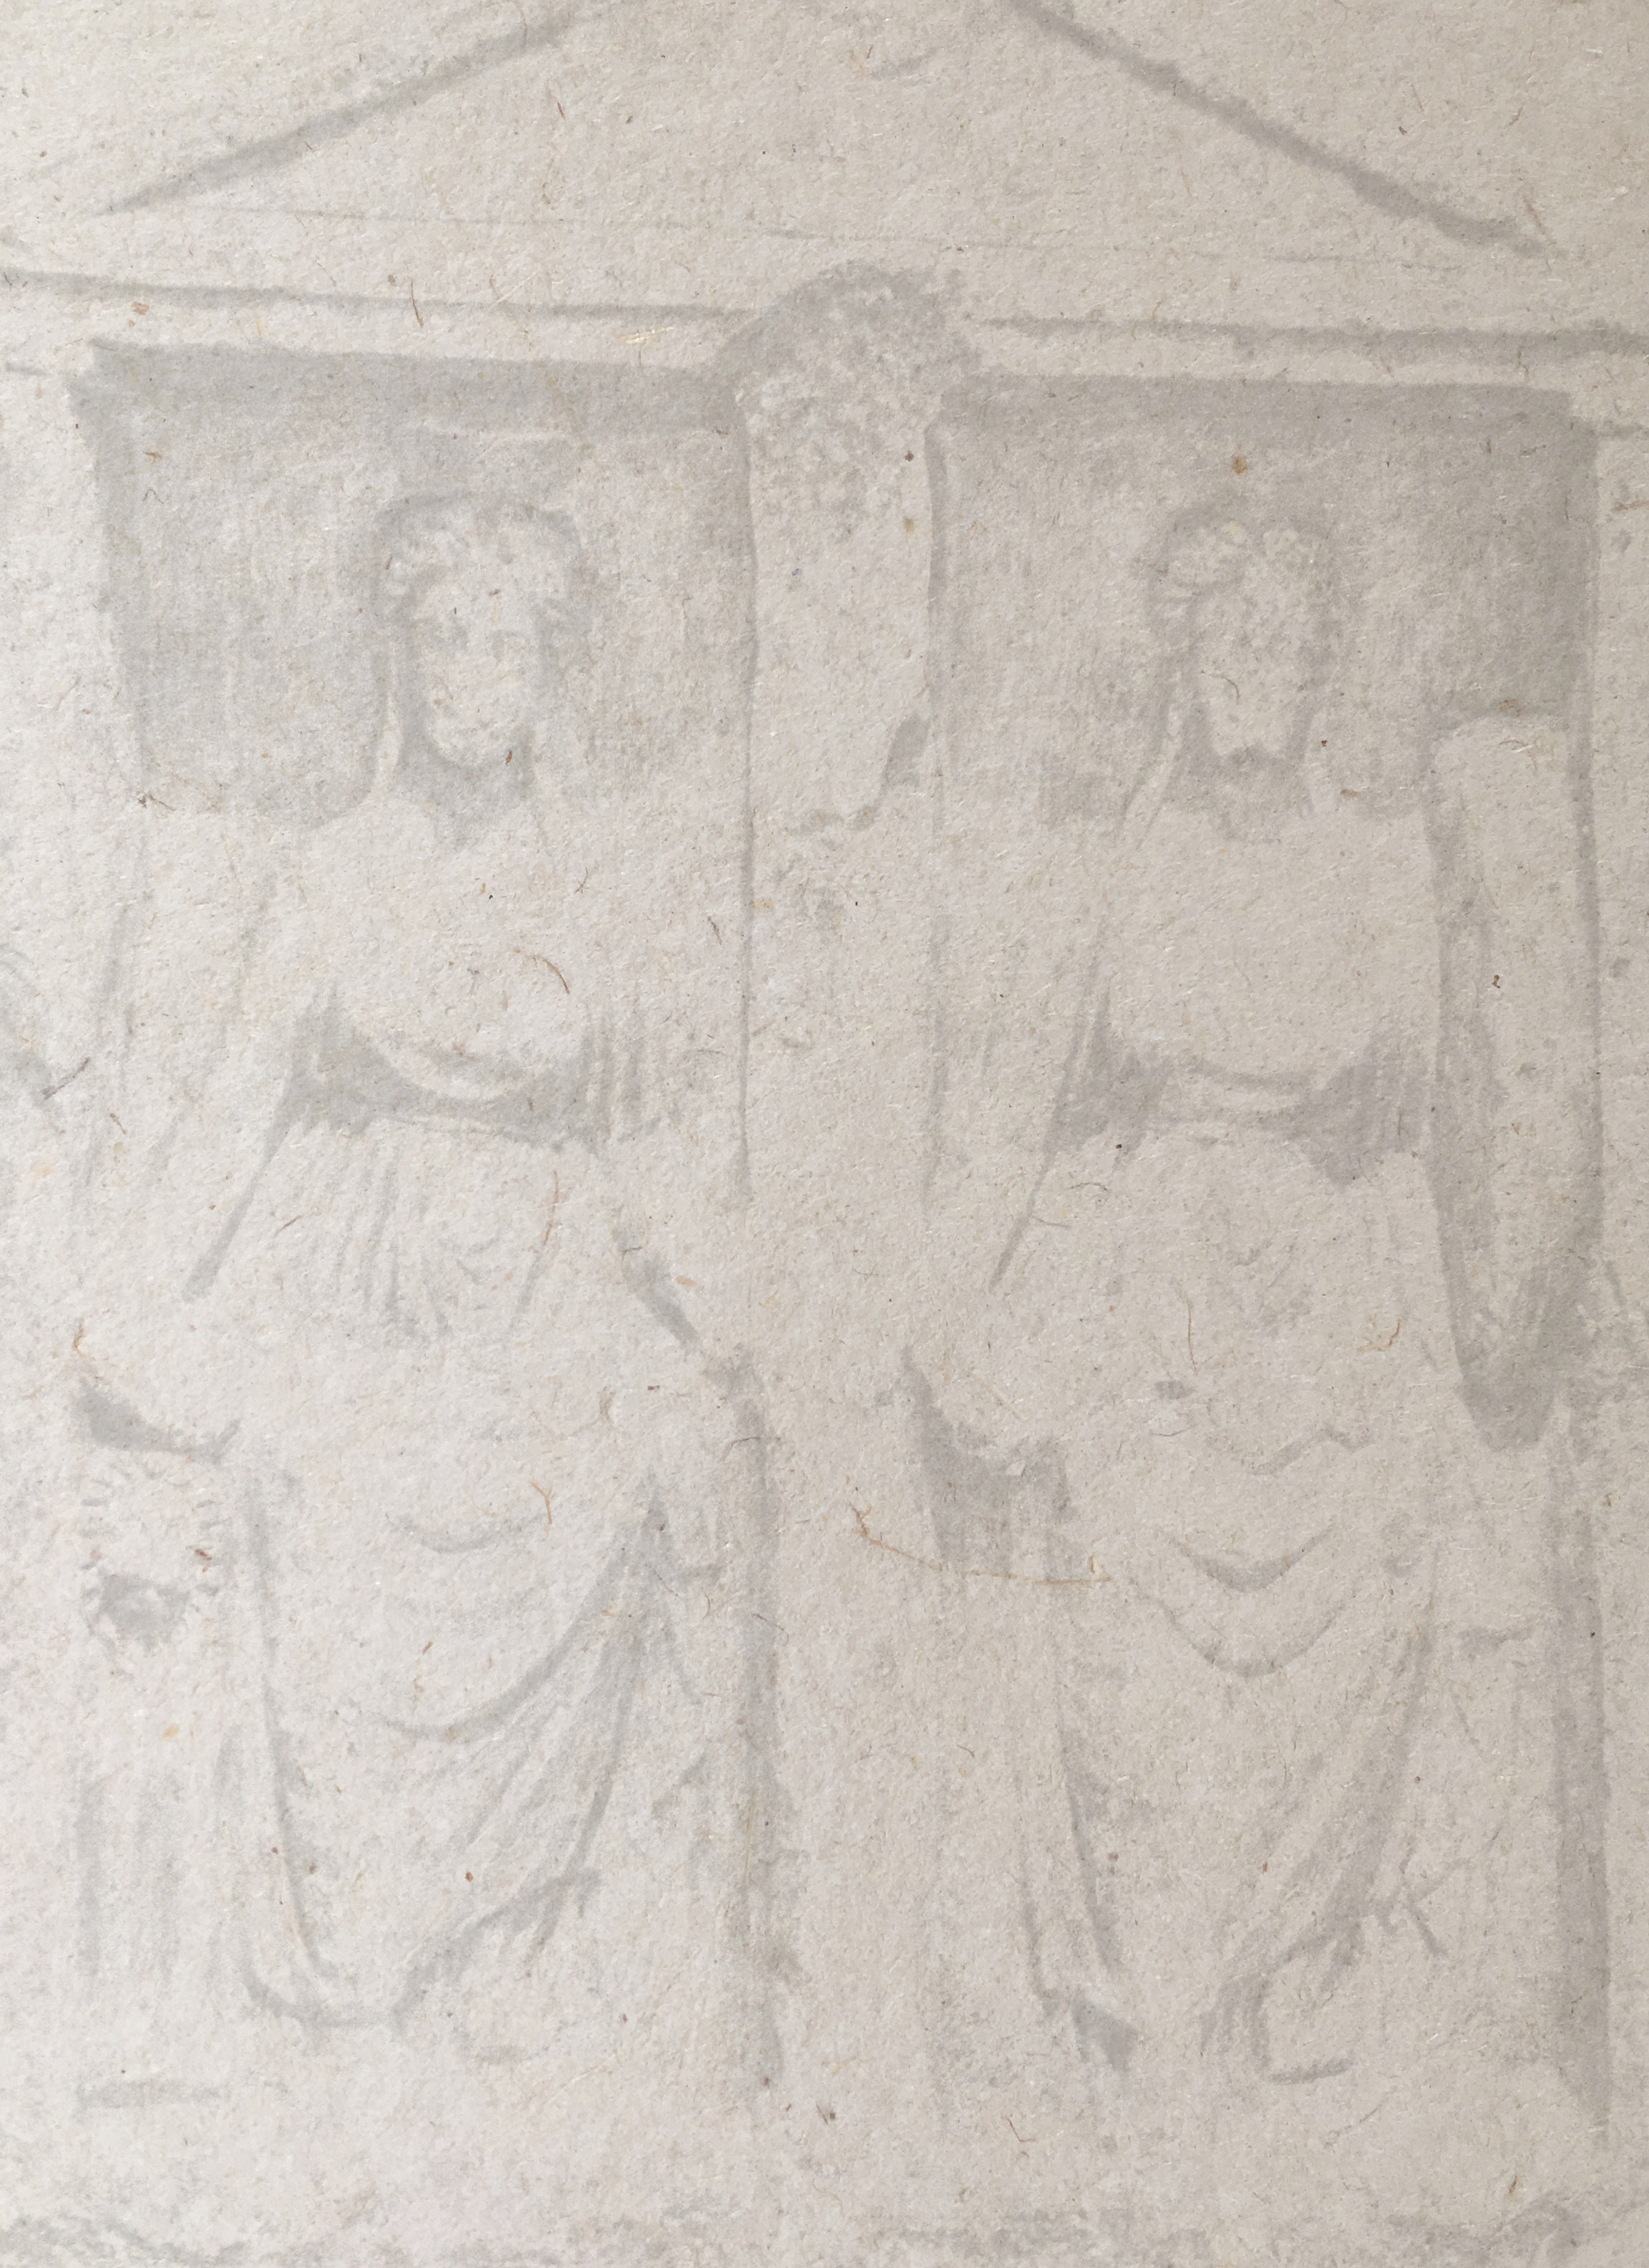
\includegraphics[width=\paperwidth,height=\paperheight]{Hemp_paper_in_Japan8.jpeg}}
\begin{titlepage} % Suppresses headers and footers on the title page
	\centering % Centre everything on the title page
	%\scshape % Use small caps for all text on the title page

	%------------------------------------------------
	%	Title
	%------------------------------------------------
	
	\rule{\textwidth}{1.6pt}\vspace*{-\baselineskip}\vspace*{2pt} % Thick horizontal rule
	\rule{\textwidth}{0.4pt} % Thin horizontal rule
	
	\vspace{1\baselineskip} % Whitespace above the title
	
	{\scshape\Huge De Matris Magnae apud \\ Romanos Cultu.}
	
	\vspace{1\baselineskip} % Whitespace above the title

	\rule{\textwidth}{0.4pt}\vspace*{-\baselineskip}\vspace{3.2pt} % Thin horizontal rule
	\rule{\textwidth}{1.6pt} % Thick horizontal rule
	
	\vspace{1\baselineskip} % Whitespace after the title block
	
	%------------------------------------------------
	%	Subtitle
	%------------------------------------------------
	
	{\scshape Dissertatio Inauguralis Philologica quam ad summos Honores ab amplissimo Ordine Philosophorum Lipsiensi rite impetrandos scripsit} % Subtitle or further description
	
	\vspace*{1\baselineskip} % Whitespace under the subtitle
	
        {\scshape \Large Henricus Rudolfus Goehler\\\normalsize Dresdensis.} % Subtitle or further description

	%------------------------------------------------
	%	Editor(s)
	%------------------------------------------------
        \vspace*{\fill}

	\vspace{1\baselineskip}

	{\small\scshape Misniae, 1886.}
	
	{\small\scshape{Typis C. E. Klinkichth et fil.}}
	
	\vspace{0.5\baselineskip} % Whitespace after the title block

        \scshape Internet Archive Online Edition% Publication year
	
	{\scshape\small Namensnennung Nicht-kommerziell Weitergabe unter gleichen Bedingungen 4.0 International} % Publisher
\end{titlepage}
\setlength{\parskip}{1mm plus1mm minus1mm}
\clearpage
\tableofcontents
\clearpage
\twocolumn
\section*{}
\paragraph{}
Antiquissimis iam temporibus\footnote{Marmor Parium v. 18 sq. Athen. 14 p. 628 B.} non modo in Lydia et Phrygia, unde cultus Matris Magnae pervenit in Graeciam, sed etiam in tota Asia cultus libidinem inflammantes viguisse notum est; inter quos si accuratius eos comparaverimus eorumque originem, quoad fieri possit, detegere conati erimus, magnam esse similitudinem facile nobis persuadebimus.\footnote{Primus accuratissime hanc disputationem instituit Movers in libro suo egregio "`die Phöniker"' vol. 1 ; de nostro cultu cf. p. 233. 560 sq. praeterea commemorabo C --- P. Tiele "`Eshmoun et les Cabires"' in "`revue de l'histoire des religions"' a. 2 tom. 3 p. 197 sq.} illum enim cultum Eshmuni, qui olim Babylone, postea Carthagine praecipue cum Cabiris, septem illis planetis, colebatur, quem narrant ab Astronoe, cui respondent numina Ashtoret,\footnote{Mueller-Wieseler denkmäler alter kunst 2, 808, quo loco Cybele Astartae similis in leone sedens et tympanum attollens sole lunaque circumdata conspicitur.} Naama (cf. Damascium 16, 2. Isidor. p. 302), amatum se ipsum mutilasse eam fugientem atque mortem obiisse, deinde Paeane adiuvante in vitam revocatum esse, non multum distare a cultu Matris Magnae et Attidis, Caelestis et Adonidis\footnote{Macrob. sat. 1, 23, 17. Ersch et Gruber encycl. 3 p. 24, 408 sq. Nonnus Dionys. 41, 22; apud Socratem in hist. eccl. 3, 23 legitur oraculum, quod Rhodiis datum erat, hoc:\\\hspace*{5mm}Ἄττιν ἱλάσκεσθαι θεὸν μέγαν ἁγνὸν Ἄδωνιν,\\\hspace*{5mm}εὔβιον, ὀλβιόδωρον, ἐυπλόκαμον Διόνυσον.} quis est qui neget ? quin etiam nescio an deum "`Eshmun"' coniungere possimus cum Aegyptio, cui nomen est "`Schmun"' (i. e. octavus cf. Gesenium in encyclop. Erschi et Gruberi s. v. "`Carthago"') eodem modo, quo recte ut mihi videtur Meinekius ad Strabonis l. 10 p. 473 (723 A) censet Cabiros (i. e. potentes) eosdem esse atque septem Aegyptiorum deos; quae si vera sunt, cultus Asiae et Aegypti antiquissimi, quos cognovimus, inter se conexi erant. nam etiam cum Aschera, quae apud Israelitas colebatur, Mater Magna comparari potest, cum ambabus non modo arbores sacrae, sed etiam galli,\footnote{Hi quoque sacerdotes deae Syriae erant, quam Matri Magnae simillimam fuisse perspicitur Luciani libello de dea Syria conscripto.} qui apud Hebraeos (reges 2, 23, 7) Cadusim appellabantur, earum ministri essent. denique Tirgata vel Atergatis eadem fere est ac Mater Magna, quippe cum in curru leonum vecta tympanumque in manibus tenens fingatur (Movers l. l. p. 583. Macrob. sat. 1, 23, 18 sq.).

Cybelen vero coluerunt Pessinuntis incolae nomine Agdistis, quod monti illi urbi proximo inditum esse fertur. Pausanias autem (7, 17, 5) et Arnobius (adv. nat. 5, 5) narrant ibi ex Iovis semine, quod in terram cecidisset, numen divinum Agdistem esse ortum; a quo ne quid mali accideret cum di timerent virilitatem ei fraude ademptam esse; ex mentula autem crevisse amygdalum, cuius fructum cum Nana Sangarii fluminis filia in sinu portavisset, praegnantem eam factam Attidem\footnote{Genetivus Attis vel Attidis esse potest cf. Keil. G. L. 4, 29, 14. 7, 480, 15; in nominativo etiam formam "`Atta"' usurpari testatur Charisius ap. Keil. 1, 67, 11.} peperisse.\footnote{Cf. hymnum in Attin ap. Bergk. P. L. 4 3 p. 686.} puerum adultum quia Agdistis amavit Pessinuntem miserunt, ut in matrimonium duceret regis filiam; attamen cum hymenaeus caneretur venit Agdistis atque Attis ad insaniam redactus se ipse mutilavit et cum eo pater nuptae. sed Agdistem paenituit facinoris eiusque precibus Iuppiter permotus concessit, ut mortui corpus numquam tabesceret. contra Diodoro teste (3, 58) in vitam reductus pater dominusque adoratus est. aliam profecto fabulam Hermesianax, qui floruit Alexandri Magni temporibus, memoriae tradidit, quam legimus in schol. ad Nic. alex. 8: ποιμὴν ἦν Φρὺξ ὁ Ἄττης ποιμαίνων δὲ καὶ ὑμνῶν τὴν μητέρα τῶν θεῶν ἐφιλήθη ὑπ᾽ αὐτῆς καὶ δὴ φαινομένη πολλάκις τιμῆς αὐτὸν ἠξίωσεν, ὁ Ζεὺς δ᾽ ἐπὶ τούτῳ δυσανασχετῶν ἀνεῖλεν αὐτὸν οὐ φανερῶς δι᾽ αἰδῶ τῆς μητρός, ἀλλὰ σῦν ἄγριον πέμψας, ἡ δὲ κατολοφυρομένη αὐτὸν ἔθαψεν, οἱ δὲ Φρύγες κατὰ τὸ ἔαρ θρηνοῦσιν αὐτόν (cf. Paus. 7, 17, 5 initio).\footnote{Omnes locos, in quibus fabula Cybeles et Attidis agitur, exponere (Ovid. fast. 4, 223 sq. Catull. 62. Serv. ad Aen. 9, 116. Tertull. ad nat. 1, 149. Arnob. adv. nat. 4, 35. Philostratus epp. 39. Sallust. de nat. d. 4. Iulian. or. 5, 165) supervacaneum est, praesertim cum Pfau in encycl. Pauly. 5, 403-405 eos composuerit. commemorare sufficit Apollinem iam apud Diodorum 3, 59, 8 in fabula reperiri et ap. Euseb. praep. ev. 2, 2, 41 sq. Marsyam cf. Mueller-Wiesler 2 tab. 41 n. 492.}

Cybele igitur (Κυβέλη, Κυβήβη) erat summa Phrygum dea, genetrix caeli et terrae, cui permulta cognomina tribuuntur, de quibus postea (part. 2) dicendum erit; coniunctus autem est cum ea Attis, symbolum morientis atque renascentis terrae. postquam autem eorum cultus per Lydiam,\footnote{De Matris Magnae cultu Sardio cf. Herodot. 5, 102. Sophocl. Phil. v. 391 sq. Plut. Them. 30 sq. Sardibus repertum est prostypon, in quo Cybele inter duos leones stans conspicitur cf. Lebas-Waddington voyage arch. en Grèce et en Asie mineure t. 3 n. 1653.} Troada, colonias Graecas,\footnote{De cultu Cyziceno cf. Herod. 4, 76. 1, 80. Apoll. Rhod. 1, 985 et schol. Schol. ad Nic. alex. 8. Zosim. 2, 31. Cedrenum p. 119 B. Marquardt. Kyzikos u. sein gebiet p. 90, 126, 186. C. I. G. 3657. Paus. 5, 13, 4. Lolling. kult der Kybele aus Plakia in mitteil. d. deutsch-archäol. inst. zu Athen 7 (1882) p. 151. De cultu Smyrnaeo cf. C. I. G. 3137, 3157, 3193, 3260, 3286, 3385-87, 3401, 3411. Strab. 10, 469. Eckhel. doctr. n. v. 2, 534. Mionnet descr. des monn. gr. suppl. 7, 400. cui deae hereditates accipere licuisse cognoscimus ex Ulpiani tit. 22, 6: deos heredes instituere non possumus praeter eos, quos senatus consultis constitutionibusve principum instituere concessum est, sicuti Iovem Tarpeium, Minervam Iliensem, Herculem Gaditanum, Dianam Efesiam, Matrem deorum Sipylenem quae Smyrnae colitur et Caelestem Selenen deam Carthaginis.} insulas\footnote{De cultu in insula Samothrace habito cf. archäol. untersuch. auf Samothrake ausgef. v. Conze, Hauser u. Niemann, Wien 1875 1. et neue archäol. unters. auf Sam. ausg. v. Conze, Hauser u. Benndorf, Wien 1880 2. Aristoph. pac. 277 sq. et schol. ibidem erat societas deorum, cui praeerat summa dea Cybelae simillima (l. l. 1 p. 21 sq.); atque etiam in nummis hoc loco repertis saepe conspicitur Mater Magna (l. l. 1 p. 11 adn. 1, 2 p. 9 adn. 1). cultum Romanis quoque placuisse testantur Plut. Luc. 13. Marc. 30 et Tac. ann. 2, 67.} in Graeciam pervenit, consentaneum erat Cybelen conecti cum Rhea, summa Graecorum dea; atque recte adnotavit Schwenck (mythologie der Griechen p. 336) Rheam non prius fuisse magnam deam, quam coniuncta esset cum Cybele Phrygia.

Quando cultus in Graeciam translatus sit, cognosci potest, si locum, qui extat apud Iulianum, coniungimus cum eis, qui apud antiquos Graecorum poetas et scriptores reperiuntur. legimus enim apud Iul. or. 5 initio haec: τίς δὲ ἡ τῶν θεῶν Μήτηρ καὶ ὁ τῆς ἁγνείας ταυτησὶ τρόπος ὅποῖος καὶ προσέτι τοῦ χάριν οὑτωσὶ τοιοῦτος ἡμῖν ἐξ ἀρχῆς κατεδείχθη, παραδοθεὶς μὲν ὑπὸ τῶν ἀρχαιοτάτων Φρυγῶν, παραδεχθεὶς δὲ πρῶτον ὑφ᾿ Ἑλλήνων καὶ τούτων οὐ τυχόντων, ἀλλ᾿ Ἀθηναίων ἔργοις διδαχθέντων, ὅτι μὴ καλῶς ἐτώθασαν ἐπὶ τῷ τελοῦντι τὰ ὄργια τῆς Μητρός; λέγονται γὰρ οὗτοι περιυβρίσαι καὶ ἀπελάσαι τὸν Γάλλον ὡς τὰ θεῖα καινοτομοῦντα κτλ. et postea ἡ γὰρ ἐν πᾶσι τοῖς καλοῖς ἡγεμὼν γενομένη τοῖς Ἕλλησιν, ἡ τοῦ Πυθίου πρόμαντις θεοῦ, (τὴν) τῆς Μητρὸς τῶν θεῶν μῆνιν ἐκέλευσεν ἱλάσκεσθαι καὶ ἀνέστη, φασίν, ἐπὶ τούτῳ τὸ μητρῷον, οὗ τοῖς Ἀθηναίοις δημοσίᾳ πάντα ἐφυλάττετο τὰ γραμματεῖα. qua fabula comparato illo Baccharum loco (vv. 64-169) Musgravio (in adn. ad Eurip. Hel. 1321) dictum videtur Cybeles sacra circa Euripidis\footnote{Bacch. 72 sq. Hipp. 141 sq. Hel. 1301 sq. frgg. 475, 589 Nauck. de nomine "`Μήτηρ ὀρεία"' cf. etiam anth. Pal. ed. Duebner 6, 173. Wieseler denkm. d. alten kunst 2, 809. Lebas-Waddington l. l. 3, 699. de dis montanis cf. in universum Migne patrol. lat. 7 p. 403 sq. 493 sq. Galerii autem Maximiani Caesaris matrem fuisse deorum montium cultricem dicit Firm. Lactantius 7 p. 211 (Migne).} aetatem Athenas permanavisse; cui sententiae obstat, quod iam antea Matrem Magnam notam fuisse Graecis apparet ex Pindari carminibus.\footnote{Strabo 10, 469. Paus. 9, 25, 3. Pind. Pyth. 3, 78. frgg. 79 48. 95 63.} quapropter Prellero\footnote{Preller griech. myth. 3 1, 537.} assentior, qui Pisistratidarum temporibus cultum in Graeciam invasisse iudicat. quod autem attinet ad fabulam a Iuliano memoriae traditam, ea ostenditur ab Atheniensibus primum cultum spretum,\footnote{Cf. Photium et Suidam s. v. μητραγύρτης. schol. ad Aristoph. Plut. 431.} sed iussu Pythiae libenter ab iis receptum esse. Athenis vero Metroon aedificatum est, quo senatus consulta aliaque decreta servabantur;\footnote{Lycurg. Leocr. 66. frg. 8. Demosth. 25, 98. schol. ad Dem. p. 47 ed. Turic. Dem. 18 ἑτ. ὑπόθ. 40. 19, 129. Aesch. 1, 60. 3, 187. schol. ad Aesch. p. 47, 4. 426, 6 in oratt. Atticis. Athen. 5, 214 C. 9, 407 C. Harpocr. s. v. Bekker anecd. gr. p. 280. Dinarch. 1, 86. frg. 24. C. I. A. 2, 404, 421, 551 etc. de Iuliano vide supra. cf. C. Curtium das metroon zu Athen als statsarchiv. 1868.} quod sacrum exornavit Phidias, ut testantur Paus. 1, 3, 5 et Arrianus peripl. 9, 1.\footnote{Attamen Plinius 36, 17 censet opus fuisse Agoracriti, Phidiae discipuli cf. Brunn gesch. d. griech. künstler 1 p. 184 sq.} cultus paulatim longe lateque fluxisse videtur; permulta enim templa commemorat Pausanias, quae postea exstructa sunt: Corinthi (2, 4, 7), Lacedaemone (3, 12, 9), Acriis (3, 22, 4), Messenae (4, 31, 9), Olympiae (5, 14, 9. 20, 9), Dymis (7, 17, 5), Patris (7, 20, 3)\footnote{Dymas et Patras cultum translatum esse a piratis, quos deduxit Pompeius in Achaiam, Stoll arbitratur (Pauly enc. real. 1, 2, 2115). Strabo 8, 378.} Megalopoli (8, 30, 4), Methydrii (8, 37, 2),\footnote{Lobeck Aglaoph. 2 p. 1139 not.} in fonte Alphei (8, 44, 3). ut autem ille artifex Atheniensium maxime egregius imagine Matris Magnae occupatus erat, ita etiam alii Graecorum huius artis periti simulacra deae quam pulcherrime reficere conati sunt, praecipue vero Damophon Messenius, qui non solum in patria imaginem eius ex marmore Pario factam posuit, sed etiam Methydrii similem, qua Phidias Athenas ornaverat (Paus. 4, 31, 6. 8, 37, 2).

Quamquam Athenienses cultu Matris Magnae reipublicae probato impedire studebant,\footnote{Plut. amat. 13, 5: οὐ δὲ ἔπηλυς ἔκ τινος βαρβαρικῆς δεισιδαιμονίας, ὥσπερ Ἄτται τινὲς καὶ Ἀδώνιοι λεγόμενοι, δι᾽ ἀνδρογύνων καὶ γυναικῶν παραδύεται καὶ κρύφα τιμὰς οὐ προσηκούσας καρπούμενος, ὥστε παρεισγραφῆς δίκην φεύγειν καὶ νοθείας τῆς ἐν θεοῖς (cf. archäol. zeitung 38, 1880 p. 9 sq.).} ne mysteria illa Phrygia acciperentur, tamen iam ex Demosthenis oratione 18, 260 (εὐοῖ σαβοῖ ὑῆς ἄττης ὑῆς ἄττης\footnote{Primus mentionem facit Attidis Theopompus poeta comicus, cuius verba ex fabula Καπηλίδων deprompta tradidit Suidas 1, 370 (cf. Meinek. frg. com. graec. 2, 2 p. 801): κολάσομαί γέ σε καὶ τὸν Ἄττιν.} Strab. 10, 3, 18) cognoscimus ea Athenas irrepsisse; nec multo post θίασοι, ὀργεῶνες, ἔρανοι\footnote{C. I. A. 2, 610, 611 ?, 614, 618, 619, 621-624, 627, 842 ?. bull. de corr. hell. 7 p. 69 sq. ? Lueders die dionysischen künstler. Foucart des associations religieuses. C. Schaefer die privatgenossenschaften im Peiraieus in "`jhrbb. f. klass. phiiologie v. 121 1880 p. 417 sq."'} in Attica constituti sunt, quorum intererat eo magis a custodia reipublicae se liberare, quo minus oraculum delphicum cultui externo resisteret.\footnote{Bouché-Leclerq histoire de la divination dans l'antiquité a. 1880 t. 3 p. 373 sq.}
\clearpage
\section{Caput 1. --- De Matris Magnae in orbe terrarum Romano cultu.}
\paragraph{}
"Civitatem eo tempore recens religio invaserat invento carmine in libris Sibyllinis propter celebrius eo anno de caelo lapidatum inspectis, quandoque hostis alienigena terrae Italiae bellum intulisset, eum pelli Italia vincique posse, si Mater Idaea a Pessinunte\footnote{Strabo 12, 568 κατεσκεύασται δ᾽ ὑπὸ τῶν Ἀτταλικῶν βασιλέων ἱεροπρεπῶς τὸ τέμενος ναῷ τε καὶ στοαῖς λευκολίθοις. ἐπιφανὲς δ᾽ ἐποίησαν Ῥωμαῖοι τὸ ἱερὸν ἀφίδρυμα ἐνθένδε τῆς θεοῦ μεταπεμψάμενοι κατὰ τοὺς τῆς Σιβύλλης χρησμούς cf. Cic. de sen. 45. Arnob. 2, 73. Amm. Marc. 22, 9, 5. Val. Max. 1, 1, 1: item Matri deum saepenumero imperatores nostri compotes victoriarum suscepta vota Pessinuntem profecti solverunt. Mionnet l. l. 4, 391.} Romam advecta foret"' (Livius 29, 10, 4 sq.). erravit sine dubio Ovidius, quem secutus est Iulianus or. Vinitio\footnote{Mommsen. G. R. M. p. 540 n. 136. eodem anno commemorat solis defectionem Olympiodorus p. 148 ed. Scheibel.} (Marquardt. röm. statsverwaltung 3, 253 adn. 2), cum dicat in libris Sibyllinis tantummodo scriptum fuisse nomen matris, quam Matrem Idaeam esse Pythia nuntiarit cf. fast. 4, 255 sq.:
\begin{quotation}
post ut Roma potens opibus iam saecula quinque

vidit et edomito sustulit orbe caput,

carminis Euboeici fatalia verba sacerdos

inspicit. inspectum tale faisse ferunt:

"`Mater abest: Matrem iubeo, Romane, requiras.

cum veniet, casta est accipienda manu."'

obscurae sortis patres ambagibus errant,

quaeve parens absit, quove petenda loco.

consulitur Paean "`Divumque arcessite Matrem,"'

inquit, "`in Idaeo est invenienda iugo."'
\end{quotation}
\paragraph{}
itaque viri nobiles M. Cornelio Cethego\footnote{Arnob. adv. nat 7, 49 ed. Vind.} P. Sempronio Tuditano coss. (u. c. 550 a. Chr. 204) ad Attalum, qui tunc rex Phrygiae erat, missi sunt atque ab eo imaginem deae\footnote{Diod. fg. 34, 32, 2. Ovid f. 4, 305. Sil. Ital. Pun. 17, 32. Lactant. 2, 7. Hieron. ad Iovin. l. 1.} acceperunt. simulatque autem haec in Italiam translata Terracinae iam adfuit, quaesitum est, qui vir optimus reipublicae esset, quoniam libri Sibyllini edixerant, ut casta manu acciperetur (Liv. 29, 14). electus autem est P. Scipio Cn. f. (Cass. Dio fr. 57, 61) adulescens, qui cum omnibus matronis Ostiam deae obviam ivit; attamen cum navis sacra Matris deum ferens Tiberino vado obhaereret nullisque viribus amoveri posset, Claudia matrona dubia ut traditur fama,\footnote{Seneca fr. 80. Cohon descr. 2 2 p. 439. C. I. L. 6, 492, ubi in parte antica arae marmoreae navis, cui imago Matris deum imposita est, conspicitur, quam Claudia Quinta, cuius statuam postea in vestibulo templi M. M. positam esse tradunt Tac. ann. 4, 64. Val. Max. 1, 8, 11, infula ad rostrum alligata ad litus trahere studet.} quae a Valerio Maximo 1, 8, 11 et ab Aur. Victore 46 confunditur cum virgine Vestali Claudia, Appii Claudii Pulchri u. c. 611 cos. filia, Cybelen oravit, ut "`ita demum se sequeretur, si sibi pudicitia constaret"' (Suet. Tib. 2), atque facile navem movit (Appian. Hann. 56. Aur. Vict. l. l.). quo religionis quasi experimento pudicissima matronarum facta est (Plin. h. n. 7, 35. Cic. de har. resp. 13, 27). M. Livius vero et C. Claudius censores ex senatus consulto aedem in monte Palatino prope ad templum Apollinis collocarunt, quam tredecim annis post M. Iunius Brutus (u. c. 563 a. Chr. 191) dedicavit; qua in re ludi Megaleses\footnote{Vellius Longus de orthogr. (Keil G. L. 7, 78, 21 sq.).} instituti sunt,\footnote{Cf. Kal. Praenest. ad d. 4 m. Aprilis. certe legendum est apud Liv. 29, 14, 13 Non. April. pro tradita lectione pridie Idus Apriles.} quos primos scaenicos fuisse confirmat Valerius Antias (Liv. 36, 36, 4). sodalitates quoque iam ab initio factae esse videntur (Cic. Cat. m. 13, 45), quarum tantummodo viri participes erant. liceat autem mihi hoc loco afferre verba Mommseni: weltgeschichtlich epochemachend war die aufnahme der phrygischen göttermutter unter die offiziell anerkannten götter der römischen gemeinde, zu der die regierung während der letzten bangen jahre des hannibalischen kriegs sich hatte verstehen müssen (R. G. 6 1, 865) et viri docti Francogallici Bouché-Leclerq in l. l. t. 4 p. 298 sq.: la sibylle infligea même aux Romains, sans doute pour leur donner uu nouveau trait de ressemblance avec les Athéniens, une des superstitions les plus antipathiques au génie national, le culte orgiastique de la Grande-Mère Phrygienne.

Quanti vero Matris Magnae cultus aestimatus sit a Romanis, liquet ex iis quae legimus apud Liv. 37, 9, 8 sq. et Polybium 21, 6, 7 ed. Hultsch. cum enim Livius in bello contra Antiochum gesto (u. c. 564 a. Chr. 190) decem navibus in statione contra Abydum relictis cum cetera classe ad Sestum oppugnandam proficisceretur, Galli duo cum sollemni habitu (μετὰ τύπων καὶ προστηθιδίων) ad eum venerunt eumque oraverunt, ut parceret urbi; quorum precibus permotus iis promisit neminem a se violatum iri; quamobrem incolae sese dediderunt. anno vero post Gn. Manlio M. Fulvio coss. ad Manlium, qui pontem fecit in flumine Sangario, missi sunt galli ab Attide et Battace sacerdotibus Matris deum Pessinuntiae sollemniter vestiti, qui victoriam illi praedicerent (Polyb. 21, 37, 5). in idem fere tempus cadunt epistolae,\footnote{Ediderunt eas primus Mordtmaan in "`Münchner sitzungsber. 1860 p. 180 sq."' cum commentario, alter Domaszewski in "`archäol. epigr. mitteilungen aus Östreich 8 1884 p. 95-101."'} quibus cognoscimus Eumenem 2 et Attalum 2, reges Pergamenos familiariter egisse cum Attide sacerdote, ut Galatiam, quae iis erepta erat, recuperarent; qua re Romani prohibere studebant, ne illi nimis potentes fierent in Asia minore (Mommsen R. G. 6 2, 50 sq.). graviora autem sunt ea, quae narrant Diodorus (fg. 36, 13) et Plutarchus (Marius 17) ad a. u. c. 652 a. Chr. 102 pertinentia, quo Battaces sacerdos deae Pessinuntiae alter Epimenides Romam venit ibique nuntiavit templo violato publice purgationes faciendas esse. sacerdotis vestimentum Diodorus l. l. sic depinxit: ἐφόρει δὲ ἐσθῆτα καὶ τὴν περὶ τὸ σῶμα ἄλλην κατασκευὴν ἑξηλλαγμένην καὶ ὑπὸ τῶν Ῥωμαίων εθῶν οὐκ ἐπιχωρουμένην χρυσοῦν τε γὰρ στέφανον εἶχεν ὑπερμεγέθη καὶ στολὴν ἀνθίνην διάχρυσον, βασιλικὴν ἀξίαν ἐπιφαίνουσαν. cum vero ille in rostris ad populum loqueretur eique metum deorum iniceret, impeditus est quominus id ageret a tribuno plebis Aulo Pompeio; attamen alter tribunus eum adiuvit atque interrogavit, quid sentiret de aede purganda; quem cum idem fere diceret, Pompeius superbe de rostris deiecit, quo facto non se, sed deam laesam esse sacerdos exclamavit. et postquam paulo post tribunus morbo affectus vita decessit, iustam esse poenam facinoris vulgus existimavit. διόπερ ὁ Βαττάκης, pergit Diodorus, λαβὼν τὴν συγχώρησιν τῆς κατὰ τὴν ἱερὰν στολὴν κατασκευῆς καὶ τιμηθεὶς ἀξιολόγοις ξενίοις, ὑπὸ πολλῶν ἀνδρῶν τε καὶ γυναικῶν προεπέμφθη τὴν ἐκ τῆς Ῥώμης ἐπάνοδον ποιούμενος. quod autem Plutarchus dicit Battacen iussu deae Romanis victoriam nuntiasse et deinde, cum ante populum verba facere vellet, a Pompeio nominatum esse ἀγύρτην, clare perspicitur ab eo permixtum esse nostrum Battacen cum illo, qui a Polybio l. l. una cum Attide appellatur.

Etsi vetitum erat cives Romanos sacerdotio Matris Magnae fungi (Dion. 2, 19), tamen iam a. u. c. 653 a. Chr. 101 civis Romanus gallus factus est.\footnote{Val. M. 7, 7, 6. cf. 1. Obsequ. 44 (ed. Iahn. p. 126) ad a. u. c. 652: servus Q. Servilii Caepionis Matri Idaeae se praecidit et trans mare exportatus, ne umquam Romae reverteretur.} Pessinuntem vero adierunt Romani, ut deae vota solverent (Val. M. 1, 1. Mommsen R. G. 6 2 p. 421), atque sacerdotium ipsum erat tam grave (Mommsen l. l. 2 p. 156), ut P. Clodius Pulcher Appii filius, cui Cicerone in exilium expulso pecunia opus erat ad res gerendas, illud, quoniam multum valuit in provinciis, Brogitaro Deiotari genero pecunia grandi venderet, ad quam rem Cicero in oratione pro Deiotaro habita alludit.\footnote{Cic. de har. resp. 13, 28. pro Sest. 26, 56. cf. epp. ad Qu. fr. 2, 7 9, 2.} idem Clodius duobus annis post (u. c. 698 a. Chr. 56) quarto die m. Aprilis curulis aedilis ludos egit Matri Magnae.\footnote{Prodigia commemorat Cass. Dio ad a. u. c 711 l. 46, 33 et ad a. u. c. 716 l. 48, 43.}

Sed nimirum in republica Romana erant, qui intellegerent cultum Matris Magnae ex more incolarum orientalium institutum populo nocere; atque extant fragmenta Varronis, quibus eum castigat cf. praeter fg. 28, 34, 36 (in sat. Menipp. rel. ed. Riese p. 131 sq.) fg. 35 (Buecheler Varr. Men. rel. 182):
\begin{quotation}
tibi typana non inani sonitu matri deum

tonimus chorus tibi nos, tibi nunc semiviri,

teretem comam volantem iactant tibi famuli,
\end{quotation}
\paragraph{}
atque etiam Lucretio homini vere Romano minime placuerunt molles modi tibiae Phrygiae.\footnote{Cf. Martial. 3, 81. 91. 7, 73. 8, 46. 9, 39.} attamen quid valuerunt illi viri contra vulgus, quod acquiescebat in cultu animos incitante, quem ne carminibus celebrarent viri veluti Catullus non caverunt, qui eo processit ut elegiam in Attin componeret, qua dicentem facit Cybelen sic:
\begin{quotation}
agedum, inquit, age ferox i, fac ut hunc furor agitet,

fac uti fororis ictu reditum in nemora ferat,

mea libere nimis, qui fugere imperia cupit,
\end{quotation}
\paragraph{}
et postremum hoc a dea petit:
\begin{quotation}
procul a mea tuos sit furor omnis, era, domo:

alios age incitatos, alios age rabidos.
\end{quotation}
\paragraph{}
tum vero eum (cf. 35, 12) secuti sunt omnes fere poetae aetatis Augusteae, Vergilius,\footnote{Ae. 9, 108. 620. 584. 10, 220. G. 4, 64. Cir. 166.} Ovidius,\footnote{Ars. a. 1, 507. met. 10, 104. 686. 696. 704. fast. 4, 223 sq. 2, 55. 3, 259. 6, 319. Ib. 403. 505. ex P. 1, 1, 39.} Propertius,\footnote{3, 17, 35. 22, 3.} Maecenas,\footnote{Anthol. Pal. n. 82.} Horatius,\footnote{Epp. 2, 1, 79. serm. 1, 2, 121.} quorum temporibus cultus noster adolevit et paulatim una cum Isidis et Mithrae cultu omnes alios removit, praesertim cum novi instituerentur dies festi, quibus Mater Magna induceretur in cultum deorum agrestium (Macrob. sat. 1, 21, 7. Plin. h. n. 18, 16); adnotandum autem est illum ludum communiter a virorum et feminarum collegiis actum esse, quibus nomen erat cannophori, cannophorae. (cap. 3).

Sed antequam ad aetatem imperatoriam transeamus, disputandum est de titulo Cyziceno, quem Boeckhius C. I. G. 3668 et multo sanius Dittenberger in sylloge 270 sic restituit: χοῦντος Βουλείδου τοῦ Μητροδώρου/Σωτηρίδης Γάλλος εὐξάμενος Μητρὶ Κοι[λανῇ]/ὑπὲρ τοῦ ἰδίου συμβίου Μάρκου Στλακκίου Μάρ[κο/υ] ὑ[ο]ῦ, τοῦ στρατευσαμένου ἐν τῇ ἐξαποστ[αλείςῃ/συ] νμαχίᾳ εἰς Λιβύην ἐπὶ Θεογνήτου τοῦ ---/--- ου ἱππάρχεω [ι] τῷ αὐτοκράτορι Γαΐῳ [Ἰουλίῳ Γαΐ]/οὐ ὑειῷ Καίσαρι ἐν νηΐ τετρήρει, σωτ[ηρίας, ὃν αἰχμα]/λωτισθέντα ἐκ Αιβύης καὶ ἀπαχθέν [τὰ εἰς δουλεί/αν] καὶ τῆς θεᾶς εἰπάσης μοι κατ᾽ [ὄναρ/ὃ] τι ᾐχμαλώτισται Μᾶρκος, ἀλ[---ἐ] (λα) ύνων ἐπὶ Κ[υρήνην?---].\footnote{Boeckhii mutationem Λοβρίνῃ nimis audacter factam summo iure Dittenb. refutavit.} quibus verbis manifestum est Soteridem gallum, cum Buleides hipparcha erat, votum pro M. Stlaccii, qui a. 46 a. Chr. in Libyam profectus ibidem in servitutem redactus est, salute susceptum solvisse, postquam ei feliciter contigit, ut amicum liberaret.

Iam vero sequitur aetas imperatoria, qua praeter scriptorum testimonia multae extant inscriptiones, quibus intellegimus cultum celeriter ad summum pervenisse fastigium.

Augustum autem, cuius uxor Livia ad Cybeles formam fingebatur,\footnote{Müller-Wieseler l. l. 1 tab. 69 n. 379.} cultui consuluisse docet monumentum Ancyranum (Mommsen. res g. d. Aug. 2 p. 82. 157), quo cognoscimus ab eo refectam aedem Matris Magnae Palatinae, quam a. u. c. 756 p. Chr. incendio deletam esse Val. Maximus 1, 8, 11 (cf. Cass. D. 55, 12. Suet. Aug. 37) narrat. cuius imperatoris aetati tribuendi sunt tituli: \emph{C. I. L. 6, 496} ONESIMVS • OLYMPIAS | LIVIA • BRISEIS • AVG • LIB • SAC | M • D • M • I, quem sic legendum esse censeo: Onesimus, Olympias, Livia, Briseis, Augusti liberti, sacerdotes Matris deum Magnae Idaeae et \emph{I. R. N. 6865} (Orelli 2984), quem posuit Cosmus aedituus Matris deum Antiocho ab imperatore Augusto gratis manumissus. ex quibus apparet sacerdotio et ministerio Augusti temporibus peregrinos et libertos fungi solere. fortasse in eandem aetatem cadit titulus feminae Atticae Mnasidi positus \emph{C. I. A. 3, 888}, quippe cum forma ἑατῆς (cf. C. I. A. 3, 550. 552. 575 sq.) imprimis Augusti aetate usitata et litterae ΘΣΣΟ ab ea alienae non fuerint (Franz. elem. epigr. gr. 1840 p. 244 sq.).

Deinde Tiberio, Claudio,\footnote{Imhoof-Blumer monnaies grecques: Lydie 172.} Caligula, Nerone (Cass. Dio 61, 20) imperatoribus nihil fere nobis de cultu traditur, quod ex parte inde explicari potest, quod Tiberius Paulina violata\footnote{Ioseph. antiqu. 18, 13, 5. Zonaras ed. Dind. p. 268. 269. Hegesipp. 2, 4. nullam autem iustam video causam, cur Lafaye "`l'histoire du culte des divinités d'Alexandrie Isis etc. 1884 p. 54 sq."' de hac fabula dubitet.} et ob alias causas Aegyptios Iudaicosque ritus compescuit, mathematicos magosque ex Italia expulit (Sueton. Tib. 36. Tac. ann. 2, 32. 85). quamquam unam inscriptionem \emph{C. I. L. 6, 2260}, quam fecit Claudia Acropolis Aug. lib. sacerdos Matris deum sibi et perenni coniugi suo Cladiano, libertis, libertabus posterisque, hisce temporibus insculptam esse concludam ex nomine Claudiae, quod accepisse videtur a gente Claudiorum imperatoria. postquam autem stirps Iulia periit, cultus denuo gliscit auctoritate atque Vespasianus templum Matris deum terrae motu\footnote{Fortasse cogitandum est de terrae motu a. 62 p. Chr. cf. Tac. ann. 15, 22: motu terrae celebre Campaniae oppidum Pompeii magna ex parte proruit; cf. etiam titulum Pompeianum C. I. L. 10, 846.} Herculanei conlapsum a. 76 p. Chr. restituit \emph{C. I. L. 10, 1406}.

Domitiano fortasse imperatore tit. \emph{C. I. L. 9, 1153} positus est a Cantria P. filia Longina, sacerdote flamina (vel flaminica) divae Iuliae Piae Augustae (Suet Dom. 22. Plin. epp. 4, 11) et Matris deum et Isidis Reginae.

Paulo vero post cultus Matris Magnae etiam in provincias invasit atque ex Gallia in Hispaniam pervenisse videtur, qua in provincia repertus est titulus \emph{C. I. L. 2, 179}, quo legitur: Matri deum Mag(nae) Idaeae Phryg(iae) Fl(avia) Tyche cernophor(a) per M. Iul(ium) Cass(ianum) et Cass(iam) Sev(eram) M. At(ilio) et Ann(io) Gal(lo) coss. (108 p. Chr.).

Ad Traiani vel Hadriani aetatem propter vocem Ulpiae spectat tit. \emph{C. I. G. 3508} Thyatirae rep., quem praecedit hic (3507): ἀγαθῇ τύχῃ/ἡ βουλὴ καὶ ὁ δῆμος/ἐτείμησαν/Οὐλπίαν Μαρκέλλαν/τὴν ἱέρειαν τῆς Ἀρτέ/μιδος, Μάρκου Οὐλπίου/Δαμᾶ παραδόξου καὶ Κανιδίας Βάσσης/θυγατέρα ἐπιτελέ/σασαν τὰ τῆς θεοῦ μυστήρια καὶ τὰς/θυσίας λαμπρῶς καὶ/πολυδαπάνως/ἀναστησάντων τὴν τει/μὴν Ἀνδρονείκου τοῦ Ἀν/δρο νείκου καὶ Στρατονεί/κης τῆς Μηνογένους/τῶν θρεψάντων/ἐκ τῶν ἰδίων sequitur alter: ἀγαθῇ τύχῃ/ἡ πατρὶς Οὐλ/πίαν Μαρκέλλαν/ἱερασαμένην/τῆς Ἀρτέμιδος,/ἀρχιέρειαν τῆς Ἀ/σίας ναῶν τῶν ἐν/Σμύρνῃ, ἀγωνο/θέτιν τρὶς τῆς/πατρίδος, ἱέρει/αν διὰ βίου τῆς/Μητρὸς τῶν θεῶν. constat igitur U. Marcellam Thyatirae natam esse, patrem eius fuisse παράδοξον,\footnote{Παράδοξο; idem est atque παραδοξονίκης cf. Plut. comp. int. Cim. et Luc. 2. C. I. G. 3, 5804. Augustin. princip. rhet. 9: tametsi quidam parum diligenter Graece loquentes paradoxa pro his, quae sunt bonae opinionis, accipiunt: unde vulgo etiam Olympionicas et ceteros victores sacrorum certaminum paradoxos vocant magis consuetudine quam ratione ducti.} matrem, quod ex nomine apparet, civem Romanam. cum vero admodum adulescens parentibus orbata esset, Andronicus eam educavit; tum Dianae sacerdos facta summo cum splendore munere functa est, ut senatus populusque statuam ei decernerent. non multo post asiarcha,\footnote{E. Kuhn: die städt. u. bürgerl. verfassung d. röm. reichs bis auf die zeiten Justinians. Lpzg. 1864. 1. p. 106 sq.} ter agonothetis patriae, a Smyniaeis perpetua Matris Magnae sacerdos creata est; quapropter altero titulo Thyatirae cives ei Smyrnae quoque statuam posuisse videntur. Patinus autem, quem secuti sunt Boeckhius et Lebas-Waddington l. l. 3, 5, magna cum probabilitate coniecit U. Marcellam sacerdotio Dianae deposito viro nupsisse atque peperisse Ulpiam Marcellam, quae commemoratur in tit. C. I. G. 3157.

Certe profecto Traiano imperatore ortus est tit. \emph{C. I. L. 3}, 1100 Apulensis, quem pro salute Augusti Matri deum Magnae sanctum T. Fl. Longinus veteranus ex decurione alae 2 Pannoniorum, decurio coloniae Dacicae, decurio municipii Napocae, decurio Kanabensium legionis 13 geminae et Claudia Candida coniunx et Flavius Longinus, Clementina Marcellina filii ex imperio pecunia sua fecerunt. cum enim nomen Sarmizegetusae absit ab hoc titulo et ab aliis eiusdem voluminis (1323. 1443. 1572 cf. C. I. L. 3 p. 228), quorum antiquissimus est 1443 ob coloniam Dacicam a. 110 p. Chr. conditam positus, atque cum postea locus appelletur colonia Ulpia Traiana Augusta Dacica Sarmizegetusa, haud dubie concludi potest titulos in quibus deest nomen Sarmiz. paulo post a. 110 p. Chr. erectos esse.

Inde ab excessu Hadriani usque ad tempora Diocletiani de cultu edocti sumus permultis titulis praesertim tauroboliacis, quorum aetas certo argumento definiri potest. priusquam autem inscriptiones explanandae sunt, opus est commemorare iam medio fere secundo saeculo patres ecclesiasticos ut in ceteros paganorum cultus, ita etiam in Matrem Magnam vehementer invectos esse; atque Octavius Minucii Felicis apologia Christiana antiquissima quae nobis tradita est abundat verbis acerrimis (cf. capp. 2, 4. 21, 1. 22, 1. 27, 6. 28, 7 ed. Vind.); afferam hoc loco illa verba quae leguntur c. 25, 9 sq.: "`sane et Acca Larentia et Flora, meretrices perpudiosae, inter morbos Romanorum et deos comprobandae. isti scilicet adversus ceteros, qui in gentibus colebantur, Romanorum imperium protulerunt: neque enim eos adversus suos homines vel Mars Thracicus vel Iuppiter Creticus vel Iuno nunc Argiva, nunc Samia, nunc Poena, vel Diana Taurica vel Mater Idaea vel Aegyptia illa non numina sed portenta fuerunt,"' et paulo post: "`ubi autem magis a sacerdotibus quam inter aras et delubra conducuntur stupra, tractantur lenocinia, adulteria meditantur?\footnote{Ioseph. antiqu. 18, 13, 5. Cosmas Hierosolymitanus ad S. Gregorii theol. v. 267 (Migne patrol. gr. 28 p. 502).} frequentius denique in aedituorum cellulis, quam in ipsis lupanaribus flagrans libido defungitur."' quem secutus est initio 3 saeculi Tertullianus, qui summa cum gravitate et eloquentia puram fidem Christianam illis numinibus paganorum libidinosis opponit.\footnote{Adv. nat. 1, 10. ad extr. 2, 8. apol. 13 sq. de corona 7. adv. Marc. 1, 13.}

Ac primo quidem titulo, qui nobis occurrit, \emph{Ann. Inst. 40 (1868) p. 367} dendrophori Ostienses, quos Matris Magnae cultum curasse ceteris titulis (p. 379. 399) satis ostenditur, imperatori Caesari T. Aelio Hadriano Antonio Aug. Pio,\footnote{De nummis Antonini Pii et Faustinae uxoris, in quibus Mater Magna visitur cf. Eckhel. 7 p. 39 sq. Cohen. 2 2, p. 417. 431. 434. 439. 382. 399. Friedlaender-Sallet das kgl. münzkabinet 2 Berl. 1877 n. 1062. de nummis M. Aurelii Antonini cf. Mionnet. l. l. 4 p. 116 sq., de n. Faustinae minoris Cohen. 2 3 p. 150. 164 sq.} pontif. max., trib. pot. 2, cos. 2, patri patriae posuerunt a. 139, quo hic iterum consul fuit. sequens titulus inest in eisdem annalibus \emph{40 p. 373}, quo Sex. Annius Merops Honoratus dendrophoris eiusdem oppidi signum terrae Matris dedicat 13 Kal. Mai. L. Cuspio Rufino T. Statio Quadrato consulibus (19 d. m. Apr. a. 142); isdem dendrophoris anno post Idib. Mai. Torquato et Herode consulibus (15 d. m. Maii a. 143) dono dedit signum Martis T. Annius Lucullus 6 vir Augustalis et quinquennalis honoratus: \emph{Ann. Inst. 40 p. 374.} denique ad eosdem dendrophoros spectat tit. \emph{Ann. Inst. 40 p. 368} valde mutilatus C. Prastina Pacato Messallino L. Annio Largo consulibus erectus (a. 147).

Primum autem taurobolium ex imperio Matris deum pro salute Antonini Augusti Pii liberorumque eius et status coloniae Lugdunensis a L. Aemilio Carpo seviro Augustali et dendrophoro Appio Annio Atilio Bradua et T. Clodio Vibio Varo consulibus (a. 160) factum est. accuratissime titulum edidit vir doctus Francogallicus Boissieu \emph{I. d. L. p. 24}; quoniam vero in parte 4 de tauroboliis disputandum mihi proposui, illo loco diligentius hunc titulum gravissimum pertractabo.

Deinde certe ante a. 169 tit. \emph{Ann. Inst. 40 p. 368} exaratus est, quo Aur. Vero Augusto, qui a. 161 post mortem Antonini Pii a fratre suo M. Aurelio Antonino Augustus electus a. 169 vita excessit Fabius Q. f. Honoratus ob honorem immunitatis dendrophoris Ostiensibus donum dedit.

Titulo insequenti, qui extat in \emph{C. I. L. 6, 3702}, Matri Idaeae T. Asuellio Marciano curatore aedium sacrarum et operum locorumque publicorum dedicatur 6 Kal. April. Pertinace et Iuliano consulibus (d. 27 m. Martii a. 175). in idem fere tempus incidit tit. \emph{C. I. L. 10, 4635}, quem Vitrasia Faustina, Pollionis consulis filia, quam a. 183 p. Chr. interfectam esse scimus (Ael. Lamprid. v. Comm. 4) ab imperatore Commodo, Matri Magnae sua pecunia fecit. cum vero Pollio a. 176 iterum consul factus sit, hoc autem titulo consul tantum nominetur, is ante a. 176 positus est. quo anno 15 Kal. Nov. (d. 18. m. Oct) complura taurobolia Lactorae percepta sunt a viris feminisque cf. \emph{Gruter, p. 30, 4. 31, 3}. Porro afferam tit. Lugdunensem (\emph{Boissieu I. d. 50. p. 28}) propter taurobolium L. Eggio Marullo et Cn. Papirio consulibus (a. 184) a Q. Aquio Anoniano pontifice perpetuo positum et tit. \emph{C. I. L. 10, 4726} Carinolae repertum, quo cognoscimus 12 Kal. Dec. Glabrione iterum consule (d. 20 m. Nov. a. 186) Munatiam Redditam sacerdotem quindecimviralem (cf. p. 3) taurobolium fecisse.

Tum vero anno 187 edocemur Hilariis\footnote{Herodian. ab exc. divi Marci 1, 1, 5: ἦρος ἀρχῇ ἑκάστου ἔτους, ὠρισμένης ἡμέρας, Μητρὶ θεῶν πομπὴν τελοῦσι Ῥωμαῖοι καὶ πάντα ὅσα παρ᾽ ἑκάστοις πλούτου σύμβολα κειμήλιά τε βασιλέων ὕλης τε ἢ τέχνης θαύυματα τῆς θεοῦ προπεμπεύει. ἄνετός τε πᾶσι δέδοται ἐξουσία παντοδαπῆς παιδιᾶς, ἔκαστός τε ὃ βούλεται σχῆμα ὑποκρίνεταί οὐδ᾽ ἔστιν οὕτω μέγα ἢ ἐξαίρετον ἀξίωμα, ὁ μὴ παντὶ τῷ βουλομένῳ ἀμφιεσθέντι ὑπάρχει παῖξαί τε καὶ κρύψαι τὴν ἀλήθειαν, ὡς μὴ ῥᾳδίως διαγνῶναι τόν τε ὄντα καὶ τὸν μιμούμενον. ἔδοξε δὴ τῷ Ματέρνῳ καιρὸς ἐπιτήδειος εἶναι ἐς τὸν τὴν ἐπιβουλὴν λαθεῖν κτλ. cf. p. 3.} Maternum quendam constituisse Commodum e medio tollere, consilio autem imperatori delato ipsum capitis damnatum esse, Commodum deae sacra obtulisse; atque verisimillimum est nummos quos habemus ex a. 191 Matri deum conservatrici Augustae (Cohen l. l. 2 3 p. 274) ob eandem causam excusos esse.\footnote{Nummi Pertinacis, in quibus Cybele conspicitur, compositi sunt ap. Cohen 2 3, 392.}

Septimii Severi temporibus tribuendi sunt hi tituli: \emph{Boissieu I. d. L. p. 31}, quo numinibus Augusti totiusque domus divinae et situ coloniae Copiae Claudiae Augustae Lugdunensis dendrophori ibi consistentes 15 Kal. Iulias Marco Sura Septimiano\footnote{Nomen imperatoris Commodi erasum est cf. Wilmanns ex. 120.} consule (d. 17 m. Iun. a. 190) taurobolium fecerunt et ibidem (\emph{Boissieu l. l. p. 33}) feminae duae Aul. Fustia Alexandria et Sergia Parthenope pro salute imperatoris L. Septimii Severi Pertinacis Augusti et, quoniam recte Boissieu verba erasa restituit, Decimi Clodii Septimii Albini Caesaris domusque divinae et statu col. Cop. Claud. Aug. Lugdunensis imp. L. Septimio Severo 2 consule (a. 194).

\emph{Ann. Inst. 40 p. 379} tit. eodem anno positus, quo M. Antius Crescens Calpurnianus V. C,\footnote{Vir clarissimus.} pontifex Vulcani et aedium sacrarum (cf. Marquardt. l. l. 3 p. 229) basim ? impositamque statuam sine vexatione ullius statuae in campo Matris deum praescripto constituere concessit aeque ac statuam poni permisit infantilem in eodem campo 8 Kal. April. C. Fulvio Plautiano 2 P. Septimio Geta 2 consulibus (d. 25 m. Martii a. 203): \emph{Ann. Inst. 40 p. 378.} anno ante patronus corporis dendrophororum Ostiensium, cuius noraen iam non legitur, ex argento pondo 3 dedit 8 Kal. Mai. Domitio Dextro 2 et Thrasea Prisco consulibus (d. 24 m. April. a. 196): \emph{Ann. Inst. 40 p. 374.}

Tit. Lugdunensis \emph{Boissieu I. d. L. p. 36}, quo pro salute imperatoris Septimii Severi et M. Aurelii Antonini Caesaris imperatoris destinati et Iul. Augustae matris castrorum (I. Capitolin. M. Aur. 26) totiusque domus divinae et statu coloniae Septicia Valeriana et Optatia Spora taurobolium fecerunt T. Sextio Laterano et L. Cuspio Rufino consulibus (a. 197).

Tit. in \emph{Orelliana sylloge 2326} extans, quo Aemilia Serapias taurobolium percepit et petram tauroboliatam posuit Idib. Maiis Annullino 2 et Frontone consulibus (d. 15 m. Maii a. 199). eodem anno vel paulo post taurobolium fecit provincia Narbonensis pro salute L. Septimii Severi Pii Pertinacis Aug. Arab. Adiabenici Parthici Maximi, quod cognomen a. 199 accepit, et M. Aurelii Antonini Aug..., quem titulum edidit Herzog in libro suo "`Gallia Narbonensis"' inscripto \emph{n. 7.}

Tit. \emph{C. I. L. 8, 2230} in Africa rep., quem Matri deum sacrum pro salute imperatorum L. Septimii Severi et M. Aurelii Augusti et P. Septimii Getae Caesaris, cuius nomen postea crasum est, et Iuliae Augustae totiusque domus divinae C. Statius Ianuarius sacerdos posuit. quoniam vero M. Aurelius\footnote{De nummis eius, qui Cybeles imaginem praebent, cf. Mionnet. 5 p. 140. Cohen 3 3 p. 122.} a. 198 Augustus et Geta eodem anno Caesar factus est, tit. inter a. 198-211 erectus esse debet.

Deinde imperatorum Septimii Severi eiusque filii M. Aurelii Antonini aetate orti sunt tituli cannophororum Ostiensium (cf. p. 3.), quorum tertius \emph{Ann. Inst. 40 p. 390 sq. n. 3} ad certum spectat annum nominibus consulum Asprorum (a. 212) additis.

Denique restat ut dicam de tit. (C. I. G. 189) \emph{C. I. A. 3, 1062}, quo consensu senatus quingentorum prytanes φυλῆς Ἀντιοχίδος Euphrosyno prostatae ob merita eius statuam decreverunt, cum Aurelius Dionysius ἄρχων ἱερεὺς Μητρὸς θεῶν καὶ Ἀγαπητοῦ erat. quaeritur autem, quis fuerit Agapetus. ac Boeckhius quidem censet Antoninum Pium intellegendum esse; attamen Dittenberger l. l. recte contradicit Minervae Poliadis nomen inter prytanes, quorum nomina titulo subscripta sunt, titulis C. I. A. 3, 1054-56 exceptis, qui pertinent ad initium saeculi tertii, nusquam praeterea reperiri; quo accedere, quod pagorum designatio desit. itaque existimo Agapetum esse Septimium Severum.

Heliogabalus autem maxime Matrem Magnam simul cum ceteris dis orientalibus\footnote{Ael. Spart. Ant. Car. 9. Cass. Dio 77, 15. 23. 78, 7. 79, 4. Ael. Lampr. Alex. Sev. 26.} coluit. narrat enim Ael. Lampridius in vita eius c. 7 non modo Matris deum sacra eum accepisse atque tauroboliatum esse, sed eo insaniae processisse (c. 28), ut leones sibi iungens Matrem Magnam se appellaret; atque apud Aur. Victorem ep. 23 legimus haec: vestalem virginem quasi matrimonio iungens suo abscissisque genitalibus Matri se Magnae sacravit. nihilominus nullus extat titulus, qui aetati eius tribui potest.

Annis Severi Alexandri\footnote{De nummis v. Mionnet. l. l. 4 p. 5.} (222-235) imperatoris pro salute eius et Iuliae Mamaeae Augustae, cuius nomen haud dubie restituendum est, et domus eorum divinae Basilicus et Mnesius criobolium fecerunt et ipsi susceperunt:\footnote{Cf. partem 4 p. 57.} \emph{tit. C. I. L. 8, 8203} in Africa repertus. alterum titulum \emph{C. I. L. 9, 1538} Beneventinum, quo non multo recentiores sunt tit. \emph{C. I. L. 9, 1539-1542} Attini et Minervae Berecyntiae sacri atque in aris tauroboliacis insculpti, 5 Id. April. Modesto 2 et Probo consulibus (d. 9 m. Aprilis a. 225) ob criobolium factum Concordia Col. lib. Ianuaria cymbalistria loco secundo posuit.

Sequuntur tit. \emph{C. I. L. 9, 3014} Teatinus, quo taurobolium de suo fecit Petronius Marcellus pro salute imporatorum Maximini Augusti et Maximi Caesaris, qui inter a. 235-238 summam imperii tenuerunt; tit. \emph{Eph. E.} 3, 15 Cordubae rep., in ara marmorea ex iussu Matris deum pro salute imperii ob taurobolium factum a Publicio Valerio Fortunato Thalamo Pio et Proculo consulibus (a. 238) erectus; videmus igitur hoc tempore et in Africa (cf. supra) et in Hispania (cf. etiam C. I. L. 2, 606, quo Huebneri sententia mihi probatur) taurobolia esse percepta; tit. \emph{C. I. L. 10, 6075} Formianus, quem Helvia Stephanis sacerdos Matris Magnae imperatore Gordiano 2 Augusto et Pompeio consulibus (a. 241) taurobolio perfecto posuit quo anno etiam exarati sunt complures tituli tauroboliaci Lactorates, quorum imus extat apud Wilmanns. exempla 124, alter ap. Orellium l. l. 2331, omnes apud Gruterum p. 29, 13. 14. 30, 1. 5.

Tum vero nobis dicendum erit de titulo \emph{C. I. G. 3886 add.}, quo legendum est:

Ὁ δῆμος ἐτείμ[ησεν]/Μόνιμον Ἀρίστων[ος]/τὸν λαμπαδάρχην [Λιός ]/Σωτῆρος καὶ Ἀπόλλ[ωνος καί]/Μηνὸς Ἀσκαηνοῦ [καί]/θεῶν Ἀνγδίστεων [καὶ Ἀγαθοῦ]/Δαίμονος καὶ εὐσεβ[ἐστάτης Σε]/βαστῆς Εἰρήνης, σ[τρατηγήσαντα]/τῆς πόλεως τὸ ἔκτον [γυμνασιαρ/χ]ήσαντα καὶ ἐγλογιστ[εύσαντα]/καὶ ἀγορανομήσαντα [καὶ εἰρηναρ]/χήσαντα [κ]αἱ παρὰ πάντα τὸν/[χρόνον πολ]ιτευσ[άμενον ἂριστα].

Cavedonius autem (Ann. Inst. 19, 136) demonstravit ἀγαθὸν δαίμονα et Σεβαστὴν Εἰρήνην referenda esse ad Otacillam et Philippum, qui inter annos 243 et 249 praeerat imperio Romano. etenim quod Letronnius φιλοδαίμονος καὶ εὐσεβεστάτης Σεβαστῆς Εἰρήνης legi vult atque refert haec verba ad Iuliam Domnam aut Iuliam Mamaeam, quia illis ambabus cognomina Felix Pia tribuuntur, huic sententiae obstat quod Felix sermone Graeco non redditur \emph{v.} φιλοδαίμων, sed semper \emph{v.} εὐτυχής.

Nunc audiamus Cyprianum,\footnote{Cf. p. 50.} qui ab a. 200 usque ad a. 257 floruit, episcopum Carthaginiensem, qua in regione Matrem Magnam cultam esse compluribus inscriptionibus confirmatur (cf. C. I. L. 8, 1649. 1776. 2230. 2633. 4846 etc. Eph. E. 5, 614), in carmine ad senatorem ex christiana religione ad idolorum servitutem conversum sic loquentem:
\begin{quotation}
quis patiatur enim te matrem credere magnam

posse deam dici rursusque putare colendam,

cuius cultores infamia turpis inurit?

namque sacerdotes tunicis muliebribus idem

interius vitium cultu exteriore fatentur,

idque licere putant quod non licet: unde per urbem

leniter incedunt mollita voce loquentes,

lassatosque tenent extenso pollice lumbos

et proprium mutant vulgato crimine sexum.

cumque suos celebrant ritus, his esse diebus

se castos memorant: at si tantummodo tunc sunt

ut perhibent casti, reliquo iam tempore quid sunt?

sed quia coguntur saltim semel esse pudici,

mente fremunt, lacerant corpus funduntque cruorem.

quale sacrum est vero quod fertur nomine sanguis?\footnote{Cf. vol. 3, 1, 21, 4 sq., quo loco verbis Minucii Felicis supra adnotatis utitur; 3, 2, 209, 14 ed. Vindob. etsi carmen h. l. c. Hartelio spurium esse videtur, tamen haud dubie hac aetate compositum est.}

nunc etiam didici, quod te non fecerit aetas,

sed tua religio calvum caligaque remota

Gallica sit pedibus molli redimita papyro.
\end{quotation}
\paragraph{}
Philippi temporibus Deae Vocontiorum ara tauroboliaca prid. Kal. Octobres Philippo Augusto et Titio consulibus (d. 30 m. Sept. a. 245) erecta est cf. \emph{Wilmanns ex. 123.} gravior autem est tit. \emph{C. I. L. 6, 488} praesentiae Matris deum a P. Septimio Felice ob coronam millesimi urbis anni (a. 247) positus. deinde quattuor annis post ortus est tit. \emph{C. I. L. 10, 3699} Cumanus, quo dendrophororum ex senatus consulto creatorum nomina subsignata sunt; Borghesius enim (opp. 3, 137. 7, 44) exposuit verba 7 Id. Oct. 3 et semel consulibus in fine tituli nominibus omissis tantummodo spectare ad a. 251 (cf. Klein. fast. consul. p. 106). cui proximus est tit. \emph{Ann. Inst. 40 p. 399}, quem quantum fieri potuit probabiliter Visconti sic supplevit:

taurob [olium crioboliumque factum]/Magnae d[eum Matri et Attini pro salute]/imp. Caesaris C. V[ibi Treboniani Galli Pii]/Fel. Aug. et[imp. Caesaris C. Vibi Asinii Galli]/Veldum[niani Volusiani Pii Fel.]/Aug. tot[iusque domus divinae et]/Senati [pro statu coloniae Ostiensis]/ex [imperio Matris deum a dendrophoris Ostiensibus]/S[acerdote?...].

Gallus autem et Volusianus imperatores erant ab a. 251 usque ad a. 254.

Iam vero transeamus ad Diocletianum, cuius aetati hi tituli assignandi sunt:

\emph{C. I. L. 10, 3698}\footnote{Cf. p. 47. tit. C. I. L. 8, 8457 Sitifensem non enumeravi in contextu, quia nobis valde mutilatus est traditus; erectus est anno prorinciae 249 i. e. a. 288 p. Chr. cf. Marqu. l. l. 1 p. 324.} Cumanus, quo edocemur consensu omnium in locum Restituti mortui Licinium Secundum, sacerdotem Matris deae Baianae creatum esse M. Magrio Basso et L. Ragonio Quintiano consulibus Kal. Iun. (d. 1 m. Iunii a. 289).

\emph{C. I. L. 6, 505} notissimus, quem L. Cornelius Scipio V. C. augur, cuius nomen redit in tit. tauroboliaco eiusdem voluminis 506, erexit taurobolio sive criobolio 3 Kal. Mart. Tusco et Annullino consulibus (d. 26 m. Febr. a. 295) perfecto.

Attamen priusquam pergam de titulis disputare, Arnobii libros 7 adversus nationes conscriptos afferam, quorum quinto Timotheum theologum secutus non modo originera nostri cultus explicare studet, sed etiam castigat impudicitiam foeditatemque, quae insunt in eo; atque summo cum taedio exclamat: o fabulam sexui inimicam semper atque infestissimam masculino, in qua secus virile non solum homines ponunt, sed pecudes etiam fiunt ex maribus matres.

Restant igitur tituli qui spectant ad quartum p. Chr. saeculum. ac primus quidem titulus \emph{C. I. L. 6, 497} Matri Magnae a Iulio Italico V. C. quindecimviro sacris faciundis taurobolio feliciter percepto Constantio et Maximiano Caesaribus 5 consulibus 18 Kal. Maias (d. 14 m. April. a. 305) positus est. nono post anno Constantino et Maximiano 3 consulibus 17 Kal. Maias (d. 15 m. April. a. 313) taurobolium fecit C. Magius Donatus Severianus V. C., pater sacrorum invicti Mithrae, hierophantes Liberi patris et Hecatarum: \emph{C. I. L. 6, 507}. maioris est momenti tit. \emph{C. I. L. 6, 508},\footnote{Cf. cap. 4. de Cerealibus vide Friedlaender. ap. Marquardt. l. l. 3 p. 479.} quo potentissimis dis Matri Magnae et Attidi Menotyranno (cf. p. 31) sacro Serapias honesta femina sacrata (quam lectionem praefero alteri "`sacerdos"' cf. C. I. L. 6, 1780) deum Matris et Proserpinae Constantino 5 et Licinio consulibus 13 Kal. Maias (d. 19 m. April. a. 319) taurobolium crioboliumque caerno Cerealibus percepit.

Quos titulos si accuratius inspexerimus, intellegemus plerosque positos esse a viris reipublicae Romanae illis temporibus clarissimis; itaque factum est, ut taurobolia crioboliaque his ipsis temporibus maxime florerent, praesertim cum imperatores subsecuti aut non resisterent iis, aut ea sacra probarent. etenim quamquam religioni Christianae Constantinus addictus erat, tamen Zosimus 2, 31 recte dicit eum nihil fecisse res divinas atque, etsi viri theologi nostrae aetatis hanc sententiam refutare conati sunt, equidem plane consentio cum Burckhardtio , qui de illo imperatore haec verba fecit (die zeit Constantins des grossen 2 p. 345): in einem genialen menschen, dem der ehrgeiz und die herrschsucht keine ruhige stunde gönnen, kann von Christentum und Heidentum, von bewusster religiosität und irreligiosität gar nicht die rede sein; ein solcher ist ganz wesentlich irreligiös, selbst wenn er sich einbilden sollte mitten in einer kirchlichen gemeinschaft zu stehn. Zosimus autem memoriae tradidit ab illo in extrema parte unius ex porticibus, quibus forum Byzantii inclusum erat, duas aedes exstructas esse collocato in altera simulacro Matris deum, quod Iasonis socii olim in monte Dindymo constituerant, idque ab eo mutatum esse, cum leones utrimque tolleret manuumque formam converteret: κατέχειν γὰρ πάλαι δοκοῦσα τοὺς λέοντας νῦν εἰς εὐχομένης μεταβέβληται σχῆμα τὴν πόλιν ἐφορῶσα καὶ περιέπουσα. nec multo post Zosimum paganitatis defensorem 1. Firmicus Maternus libellum "`de errore profanarum religionum"' composuit, quem Constantini filiis dicavit, quos admonuit ut tantae calamitatis errorem abicerent et studia mentis profanae tandem aliquando desererent. quomodo autem ille, qui c. 3 cultum Attidis explanare instituit, cultus orientales ortos esse censeat, apparet ex eo quod c. 13, 2 Serapin coniungit cum fabula illa Iosephi, cui, quia Sarrae pronepos fuerit, post mortem eius nomen Σάρρας παῖς (Σάραπις) inditum sit, et c. 3 hariolatur "`Phryges, ut annuum sibi sacrorum ordinem facerent, mulieris divitis ac reginae suae amorem, quae fastus amati adulescentis tyrannice voluisset ulcisci, cum luctibus annuis consecrasse et iactavisse, aut ut satis iratae mulieri facerent aut ut paenitenti solacium quaererent, eum quem paulo ante sepelierant revixisse, et cum mulieris animus ex impatientia nimii amoris arderet, mortuo adulescenti templa fecisse."' hoc quidem impetravit, ut a. 341 Constantius ediceret, ut sacrificiorum aboleretur insania (cod. Theodos. 16, 10, 2), atque a. 346, ut cuncti sacrificiis abstinerent et siquis aliquid forte huiusmodi perpetravisset gladio ultore sterneretur (cod. Theodos. 16, 10, 4). attamen cultus denuo renatus est Iuliano imperatore (a. 361-363), qui ut Matris deum, quam oratione quinta laudibus extulit,\footnote{Cf. p. 232 ed. Hertlein: ὦ θεῶν καὶ ἀνθρώπων μῆτερ..., ὦ πάντων μὲν ἀγαθῶν τοῖς νοεροῖς ἡγδυμένη θεοῖς, πάντων δὲ ἀποπληροῦσα τὸν αἰσθητὸν κόσμον, πάντα δὲ ἡμῖν ἐν πᾶσιν ἀγαθὰ χαρισαμένη, δίδου πᾶσι μὲν ἀνθρώποις εὐδαιμονίαν, ἧς τὸ κεφάλαιον ἡ τῶν θεῶν γνῶσίς ἐστι κτλ. Amm. Marc. 22. 9, 5-8. Libanius in orat. consulari p. 247 et in monodia de Iuliani obitu p. 254.} sacra florerent summam operam navavit ita ut Callixenum bene de sacerdotiis meritum duplici et Demetris et Matris Magnae Pessinuntiae sacerdotio honoraret atque Arsacio Galatiae summo sacerdoti imperaret, ut Pessinuntis incolas ad Matrem Magnam colendam impelleret; dicit enim (ep. 49):
\begin{quotation}
\hspace*{5mm}οὐ γάρ μοι θέμις ἐστὶ κομιζέμεν οὐδ᾽ ἐλεαίρειν

\hspace*{5mm}ἀνέρας, οἵ κε θεοῖσιν ἀπέχθωντ᾽ ἀθανάτοισιν.

πείθε τοίνυν αὐτούς, εἰ τῆς παρ᾽ ἐμοῦ κηδεμονίας ἀντέχονται,

πανδημεὶ τῆς Μητρὸς τῶν θεῶν ἱκέτας γενέσθαι.
\end{quotation}
\paragraph{}
Quo mortuo praecipue Theodosius\footnote{Cod. Theod. 16, 7, 1. 10, 7. 10. 11. 12. Symm. epp. 10, 61. Liban. ὑπὲρ τῶν ἱερῶν. Socrat. hist. eccl. 5, 16. Zosim. 4, 33. 37. 59.} (a. 379-395) religiones paganas funditus evertere conatus est; quamquam ipsius temporibus viri praeclarissimi Symmachus\footnote{Laudat. in Valentinianum 2 (monum. Germ. h. auctt. antiquiss. 6, 1 ed. O. Seeck.): quanto parcior vestri numinis cultus est quam deorum! illis singula templa fundantur et sua cuique locantur altaria. inde ut arbitror maluerunt dispares ritus, ne in consortium cogerentur: nulli cum altero fas est dicaro pulvinar; hunc phrygius antistes placat, hunc pontifex; illas castae matres tuentur aras, has infulata virgo custodit; sumpserunt nomina diversa tot flamines, no possent dis pluribus esso communes. ipsas nobilium divisere gentes: Pinarios Hercules occupavit, Idaea Mater legit hospites Scipiones, Veneriis sacris famulata est domus Iulia.} (cos. a. 391), Vettius Agorius Praetextatus\footnote{cf. p. 59.} († cos. designatus a. 385), Virius Nicomachus Flavianus\footnote{C. I. L. 6, 1782. Teuffel, gesch. d. röm. litt. 4 p. 1007. § 428 adn. 1-4.} (cos. a. 394) cultui pagano dediti erant. in quos invehitur anonymus auctor carminis codicis Parisini n. 8084, quod a Mommseno in Hermae vol. 4 publici iuris optime factum hac aetate compositum est.

Denique de titulis ad haec tempora pertinentibus dicam: \emph{Tit. C. I. L. 6, 1675}, quem Alfenius Ceionius Iulianus Kamenius V. C. tauroboliatus ante a. 333 posuit, cum hoc anno munere praefecturae urbis fungeretur, quod in titulo non commemoratur. cui proximus est tit. \emph{C. I. L. 6, 498} in ara tauroboliaca extans, quam Antoninus V. C. pontifex et quindecimvir sacris faciundis taurobolio confecto 3 Kal. Maias Fl. Anicio et Nigriniano consulibus (d. 29 m. April. a. 350) feliciter consecravit. similem aram dicavit in tit. bilingui \emph{C. I. L. 6, 509} Petronius Apollodorus V. C. pontifex maior, quindecimvir sacris faciundis, pater sacrorum dei invicti Mithrae taurobolio criobolioque percepto una cum Rufa Volusiana C. filia (vel potius clarissima femina?) coniuge 16 Kal. Iul. Valentiniano et Valente Augustis 3 consulibus (d. 16 m. Iunii a. 370); probabile autem est Rufam Volusianam fuisse filiam C. Rufi Volusiani V. C. patris, hierophantae, prophetae Isidis, pontificis dei Solis, qui votum solvit ara marmorea, cuius inscriptio legitur \emph{C. I. L. 6, 846}.

Matri autem deum Magnae Idaeae summae parenti et Hermae et Attidi Menotyranno invicto Clodius Hermogenianus Caesarius V. C., qui idem esse videtur atque ille comes rerum privatarum in cod. Theod. 10, 1, 8 a. 364 commemoratus, proconsul Africae, praefectus urbis Romae, quindecimvir sacris faciundis taurobolio criobolioque perfecto 14 Kal. Aug. Gratiano Aug. 3 et Aequitio consulibus (d. 19 m. Iulii a. 374) aram dicavit: \emph{C. I. L. 6, 499}.

Porro cadunt in annum 376:

\emph{Tit. C. I. L. 6, 504 et 510}, quorum unum Ulpius Egnatius Faventinus V. C. taurobolio criobolioque Id. Aug. (d. 13 m. Aug.) percepto posuit, alterum eodem die Sextilius Agesilaus Aedesius V. C. taurobolio criobolioque in aeternum renatus (cf. p. 53. 57. 59).

Anno vero post exarati sunt:

Tit. \emph{C. I. L. 6, 511} metricus Matri deum Magnae Idaeae et Attidi Menotyranno a Sabino 4 Id. Mart. (d. 12 m. Martii) et tit. \emph{C. I. L. 6, 500} iisdem deis a Caelio Hilariano V. C. 3 Id. Maias (d. 13 m. Maii).

Sequitur tit. \emph{C. I. L. 6, 1780} Fabiae Aconiae Paulinae clarissimae feminae, filiae Aconii Catullini V. C., uxori Vettii Praetextati V. C., quae multis deorum dearumque sacris initiata erat, tauroboliatae positus; cum vero munus praefecturae urbis, quo coniunx eius a. 384 functus est (cod. Theod. 6, 5, 2. cod. Iustin. 1, 54, 5), in titulo coramemoretur idemque consul designatus appelletur, quo facto vita excessit anno eodem vel sequenti\footnote{Mortem eius luget Symmachus epp. 10, 30 sq.} titulum nostrum non ante a. 384 erectum esse constat.

Paulo post ortus est tit. \emph{Bull. inst. arch. 1884 p. 56 sq.}, quera posuisse videtur 2 Non. Sept. Arcadio et Fl. Bautone V. C. consulibus (d. 4 m. Sept. a. 385)\footnote{Sequuntur versus pulcherrimi:\\\hspace*{10mm}inter avos proavosque tuos sanctumque parentem\\\hspace*{10mm}virtutum meritis et honoribus emicuisti,\\\hspace*{10mm}ornamentum ingens generis magnique senatus;\\\hspace*{10mm}sed raptus propere liquisti, sancte Kameni,\\\hspace*{10mm}aeternos fletus obiens iuvenilibus annis.\\\hspace*{10mm}te dulcis coniunx lacrimis noctesque diesque\\\hspace*{10mm}cum parvis deflet natis solacia vitae,\\\hspace*{10mm}amisisse dolens casto viduata cubili,\\\hspace*{10mm}quae tamen extremum munus solacia luctus\\\hspace*{10mm}omnibus obsequiis omat decoratque sepulcrum.} uxor coniugi suo Alfenio Ceionio Iuliano Kamenio anno 43 mortuo, quem eundem fuisse atque illum Alfenium, de quo supra dixi (p. 25), nequaquam verisimile est; quod si acciperemus, aut multo post eius mortem sepulcrum factum aut numerus annorum a lapicida falso insculptus esset, cui sententiae obstant verba: "`obiens iuvenilibus annis"' et "`te coniunx cum parvis deflet natis."' itaque arbitror illum Ceionium patrem nostri fuisse, qui uterque sanctus nominatur atque eosdem honores percurrit.

Tum vero tit. \emph{C. I. L. 6, 1778} Vettio Agorio Praetextato V. C. tauroboliato Kal. Febr. Fl. Valentiniano Aug. 3 et Eutropio consulibus (d. 1 m. Febr. a. 387) positus est et tit. \emph{C. I. L. 6, 1779} eidem et Aconiae Fabiae Paulinae uxori (cf. supra), qui coniuncti vixerunt annos 40 ad eundem annum spectat tit. \emph{C. I. A. 3, 173}, quo consulibus Onorio et Euodio 6 Kal. Iun. (d. 27 m. Maii), cum Hermogenes archon\footnote{Cf. Henzen. bull. inst. arch. 1867 p. 174.} fuit, Musonius Athenis taurobolium percepit; quoniam vero tit. \emph{C. I. A. 3, 172}\footnote{V. Keil. Philol. 23, 607. archäol. zeitung 1863 p. 74. arch. anzeiger 1867. Maurer de aris Graecorum pluribus deis in commune positis. Darmstadii 1885 p. 101. Kaibel epigr. gr. 822.} primum taurobolium Athenis factum commemoratur, manifestum est hunc titulum illo antiquiorem esse atque Iuliani fortasse aetate exaratum.

Restant duo tituli: \emph{C. I. L. 6, 503} a L. Ragonio Venusto V. C. taurobolio criobolioque percepto 10 Kal. Iun. Valentiniano Aug. 4 et Neoterio consulibus (d. 23. m. Maii a. 390) et tit. \emph{C. I. L. 6, 512} eodem anno et die a Ceionio Rufio Volusiano V. C. iterato annis 20 expletis taurobolio dedicatus.

Quamquam nullus titulus ad posteriorem aetatem pertinere videtur,\footnote{Titulum C. I. L. 6, 736 non attuli propterea quod multa in eo suspiciosa sunt.} tamen cultum Matris Magnae ceterorumque deorum orientalium\footnote{Cf. tit. C. I. G. 4945. 4946, qui ad Isidis cultum spectantes annis 449 et 453 (Boeckhius ambos tribuit anno 453) positi sunt.} aliquanto post viguisse scriptis patrum ecclesiasticorum Ambrosii (cf. Migne patrol. lat. 16 p. 980) et Augustini de civitate dei satis confimiatur (2, 4).

Priusquam finem huius partis absolvam, de Matris Magnae apud Germanos cultu brevia addere mihi liceat. Tacitus enim dicit in Germ. c. 45: "`ergo iam dextro Suebici maris litore Aestiorum gentes adluuntur, quibus ritus habitusque Sueborum, lingua Britanniae propior. Matrem deum venerantur. insigne superstitionis formas aprorum gestant: id pro armis omnique tutela securum deae cultorem etiam inter hostis praestat."' quibus cum verbis conferendum est id quod legimus c. 9: "`pars Sueborum Isidi sacrificat."' notum autem est Germanorum deos a Romanis libenter cum suis comparatos esse ita ut Mercurium Martem Herculem ab illis cultos esse memoriae tradat Tacitus. quaeritur quae nomina Isis et Mater deum apud Germanos habuerint. Isidi autem similem fuisse deam Suebis sacram, quae Zise nominabatur non sine aliqua probabilitate Grimm (deutsche myth. 2 1 p. 236 sq. 275 sq. cf. O. Schade die sage von der heiligen Ursula etc. 1854 p. 71 sqq.) coniecit. attamen quae dea erat Mater deum? equidem arbitror eam fuisse terram matrem, quae in titulis nobis occurrit nomine Hludanae (cf. Brambach. C. I. Rh. indicem s. h. v.); nec quod Schwenck (mythol. d. Germanen p. 179) exposuit cogitandum esse, quia Tacitus l. l. aprorum formas commemorat, de dea "`Frigg"' vel "`Freya,"' cuius cognomen erat "`Syr"' (mutterschwein), hoc meae sententiae obstat, quoniam etiam "`Freya"' nulla alia dea est nisi mater terra.\footnote{Mater Magna in titulo C. I. L. 8, 5524 cum Terra Matre et Aerecura, de quo nomine egit Mommsenus in archäol. ztg. a. 1865 p. 88 (aes --- curare geldschafferin), haud dubie propterea coniungitur, quod illa numina ei similia erant.}
\clearpage
\section{Caput 2. --- De reliquis rebus ad cultum pertinentibus.}
\paragraph{}
Ac primum quidem hoc capite, quoniam initio dissertatiunculae exposui Cybelen confusam esse cum aliis deabus Asiae, videamus, cum quibus Romanorum numinibus Cybele et Attis coniungantur. reperimus autem tria numina, quae ei similia fuisse videntur\footnote{Graeci, ut hoc addam, Cybelen confuderunt cum Rhea cf. p. 3, cum Hecato cf. schol. Lycophr. 77. Theodoret. Ther. serm. 1. Baumstark encycl. Paul. s. v., cum Cerere graeca cf. Euripidis locos p. 4 adn. 1. in locis Aristoph. Lemn. frg. 332 ed. Dind. et Plut. de virtut. mul. 9 Cybele conversa esse videtur in formam Artemidis Brauroniae.}; ex imaginibus\footnote{Cf. Mueller-Wieseler l. l. 2, 807, quo Cybele a leonibus circumdata dextera spicas et papaver tenens conspicitur; et Livia quoquo sub imagine Cybeles spicis Cereris ornatum est cf. p. 11. C. I. L. 5, 796 M. D. M. Cereriae votum solvit Fruticia Thymele.} enim perspicitur Cererem eandem habitam esse a Romanis ac Cybelen atque scriptores narrant\footnote{Macrob. 1, 12, 20 sq. Arnob. 3, 32 cf. Tertull. adv. nat. 2, 12.} Maiam vel Opem fuisse alteram Matrem Magnam. quamobrem etiam explicari potest, cur tit. C. I. L. 6, 499 Matri Magnae et Hermae et Attidi positus sit; cognoscimus enim Matrem Magnam hoc loco esse Maiam, quam cum Maia Hermae matre a Romanis commixtam esse constat.\footnote{Preller röm. myth. p. 597. Mionnet 4, 166 quo Cybele Hermen sinistra manu tenet. Jhrbb. d. vereins v. altertumsfr. im Rheinl. 23 p. 53 tab. 3, ubi Mater Magna in sinistra parte circumdatur ab Herme, in dextera ab Attide. vix autem hoc in prostypo cogitandum est de Herme-Cadmilo (Conze archäol. ztg. 1880 p. 1 sq.).} Romana quoque aetate factum est, ut Mater Magna vel pro Diana vel pro Minerva Graecorum haberetur, quo referendi sunt tit. C. I. L. 9, 1538-1542 Attidi et Minervae Berecyntiae dedicati.\footnote{Preller röm. myth. p. 739.} Attin autem, in cuius locum saepe alios\footnote{Bacchum, Sabazium, cuius mater Cybele nominatur a Strabone 10 p. 470 sq., Panem cf. Mueller-Wieseler l. l. tab. 43 n. 543. Lucian. Icaromenipp. 27, Hermen-Cadmilum cf. Conze archäol. ztg. 1880 p. 1 sq.} Graeci substituunt, Romani cum Hercule confudisse videntur; quo spectant ea quae legimus apud Tertullianum 1, 361 (Migne): vidimus aliquando castratum Attin, illum deum ex Pessinunte, qui vivus ardebat, Herculem induerat, ad quem locum Le Nourry addit: in crudelibus illis spectaculis homines et sceleratos sumpta vel Atydis vel Herculis forma repraesentare castratum Atyn et vivum Herculem combustum.\footnote{Dissert. de Arnob. l. c. 14 art. 2. cap. 18 art. 1.} Herculem autera fuisse Cybeles comitem ex Paus. 9, 19, 28, Strab. 10, 473, Diod. 5, 64 intellegimus (cf. Stuhr. religionssystem d. Hell. p. 482).

Deinde de cognominibus, quae Matri Magnae indita sunt a scriptoribus et in nummis,\footnote{Be cognominibus, quae insunt in titulis cf. indicem s. v. Mater Magna.} verba ita faciamus ut, quo plenior exhibeatur conspectus, ne Graecorum quidem testimonia negligamus; reperiuntur haec:

θεὰ Φρυγία Strabo 10, 469. Diog. 50. 6, 1. Lucian. amor. 42. ἡ Φρυγία δαίμων Arr. tact. 33, 4. dea Phrygia Verg. Ae. 7, 39. mater Phrygia Arnob. 2, 73. ἡ μεγίστη Μήτηρ θεὰ ἡ Φρυγία Iulian. epp. 21.

Ἰδαία (Idaea) Strabo 1, 45. 10, 469. Eur. Or. 1453. Apoll. Rhod. 1, 1128. Dion. H. 2, 19. Verg. Ae. 10, 252. Lucret. 2, 611. Liv. 29, 10. Hygin. fab. Hesych. s. v. Apul. met. 8, 25 (ed. Eyssenh.).

Δινδυμήνη (Dindymene) Strabo 10, 469. Herod. 1, 80. Paus. 7, 17, 5. Apoll. Rh. 1, 1125. Hor. od. 1, 16, 5. Martial. 8, 81.

Σιπυληνή Strabo 10, 469. Eckhel d. n. v. 2, 534.

Ἀσπορ[δ]ηνή Strabo 10, 469.

Berecyntia mater (deum genetrix) Verg. Ae. 6, 784. Arnob. 5, 9. 13. Ovid. f. 4, 335. August. d. civ. d. 2, 4. carmen cod. Paris. 8084 v. 73 (Herm. 4, 356).

Λοβρίνη Nic. Alex. 7 et schol.

Πεσσινουντία Herod. 1. 11, 3. Strabo. 10, 469. Pessinuntia Apul. met. 10, 5 ed. Eyssenh. Pessinuntia Dindymene Arnob. 4, 35. cf. Mionnet. 4, 391.

Πλακιανή Paus. 5, 13, 4.

Ἀνδειρηνή Steph. Byz. s. v. Strabo 13, 614.

Mygdonia Val. Flacc. 2, 46.

Mater Iliaca Prudent. c. Symm. 1, 629.

Βριμώ Theodor. Therap. serm. 1. cf. Orph. Arg. v. 16 sq.

θεὰ Φασιανή Arrian. peripl. 9.

Cybeleia mater Ovid. Ib. 453.

Mater deum salutaris Cohen 2 2 p. 431.

ἀνταία δαίμων Apoll. Rh. 1, 1141.

ἀνταία μήτηρ Hesych. s. v. Etymol. m. s. v. Orph. hymn. 41, 1.

ζωογόνος Iul. or. 5 p. 180 (ed. Hertl.).

caelicolum genetrix cf. Sil. Ital. 17, 3; de voce "`Μήτερ Ὀρεία"' cf. p. 4 adn. 1, de voce "`mater deum conservatrix"' p. 17, de voce "`Mater turrita"' p. 46. deinde tituli C. I. A. 2, 134-137, ubi Mater Magna εὐάντητος ἰατρείνη appellatur, nos docent eam etiam morbos sanavisse. attamen quid significet nomen "`Mater Magna Cognationis,"' quod in duobus titulis Salonis rep. extat (archäol. epigr. mitt. aus Östr. 8 p. 111), nescio.

Quod pertinet ad Attidis cognomina, haec adnotatione digna mihi esse videntur:

Berecyntius Attis Pers. sat. 1, 93.

Πάπ(π)ας Herod. 4, 59. hymn. in Attin. Diod. 3, 58, 4. Eustath. in Hom. 2. ε, 408.

βασιλεὺς Ἄττις Iulian. or. 5 p. 168 C. 169 C.

ὑπουργὸς τῇ Μητρὶ καὶ ἡνίοχος Iul. l. l. p. 171 C. atque in titulis nominatur Attis Menotyrannus (Μηνὸς-τύραννος), quia idem est ac Sol.\footnote{C. I. G. 3439 Ζεὺς Μηνιτύραννος logitur. Macrob. sat. 1, 21. Arnob. 5, 42. Stuhr l. l. p. 130. Jhrbb. d. ver. v. altertumsfr. i. Rheinl. 23 p. 53 sq. Lebas-Wadd. l. l. 3 adn. ad n. 668. Maurer de aris Graecorum pluribus deis in commune positis. Darmstadii 1885 p. 103. Cybele quoque lunae domina habita esse videtur quia in prostypo (archäol. epigr. mitt. aus Östr. 1, 1877 p. 14 tab. 3) lunae falx in capite conspicitur.}

Nunc vero breviter exponam, quomodo scriptores posterioris aetatis et philosophi et patres ecclesiastici fabulam Matris Magnae et Attidis interpretati sint. Iulianus autem in or. 5 p. 161 D. et Sallustius de natura deorum 4\footnote{Mater itaque deorum vivifica dea est ideoque Mater vocatur: Attis eorum quae fiunt et corrumpuntur artifex; huic apud Gallum flumen compertus traditur. Gallus enim Galaxiam seu lacteum orbem, unde corpus passionibus obnoxium descendit, indicat. primis autem diis secundos perficientibus Mater Attidis amore correpta caelestes illi facultates largitur: is enim pileus est. Attis autem Nympham deperit: cum Nymphae generationi praesint; nam quodcumque fit, fluit. quoniam vero generatio sistenda erat, ne extrema semper deterius progignerent, ea molitus opifex facultates ad generandum fecundas dimittens iterum cum diis coniungitur. et haec quidem numquam facta sunt, cum semper sint et mens quidem omnia simul conspicit; at sermo haec quidem prius, illa posterius effert. hac ratione cum aptissime mundo fabula respondeat, nos quanam alia ratione nitidius ornaremur quam mundum imitantes? propter illa festum diem agimus. et primum sane ipsi e coelo delapsi et cum Nympha consuescentes in maerore vivimus a frumento alioque crasso et sordido cibo abstinentes, quandoquidem utraque animo sunt contraria. deinceps arboris incisiones et ieiunium, quasi nos ipsi ulteriorom generationis progressum amputaremus: tandem ex lacte alimentum, quasi renasceremur. hinc festivitates (hilaria) et coronae et ad deos veluti reditio. hisce et tempus, quo fiunt, testimonium exhibet; circa enim veris aequinoctium ea quae diximus conficiuntur, cum quae fiunt fieri cessant, diesque nocte magis ac magis protenditur: quod animis, qui ad sublimiora gradum faciunt, proprium est. sic circa oppositum aequinoctium raptus Proserpinae successisse fingitur, qui descensus ost animorum.} putant ea ostendi, quomodo anima de coelo ad corpus humanura deveniat atque postremo ad deos redeat, aut quoniam ambo student philosophiae, quam novam Platonicam nominamus, ea per allegoriam significari, quomodo numen divinum paulatim atque gradatim usque ad materiem, quae ἵλη appellatur, descendat rursusque ea ascendat ad sublimiora.\footnote{Cf. Visconti. ann. inst. 41 (1869) p. 226.} aliquanto ante aliter explicavit fabulam Porphyrius ap. Euseb. praep. ev. 3, 7 sic: Ἄττις δὲ καὶ Ἄδωνις τῆς τῶν καρπῶν εἰσι ἀναλογίᾳ προσήκοντες ἀλλ᾽ ὁ μὲν Ἄττις τῶν κατὰ τὸ ἕαρ προφαινομένων ἀνθέων καὶ πρὶν τελεσιγονῆσαι διαρρεόντων --- ἔνθεν καὶ τὴν τῶν αἰδοίων ἀποκοπὴν αὐτῷ προσανέθεσαν μὴ φθασάντων ἐλθεῖν τῶν καρπῶν εἰς τὴν σπεῥματικὴν τελείωσιν --- ὁ δὲ Ἄδωνις τῆς τῶν τελείων καρπῶν ἐκτομῆς σύμβολον; quem secuti sunt Lactantius inst. d. 1, 17, Iul. Firm. Maternus 3, 5, Augustinus de civ. dei 7, 25. 2, 4. 6, 8 (cf. C. I. L. 6, 509 = Kaibel epigr. gr. 824). quo loco etiam commemorabo Isidem, cuius cultus haud scio an maxime floruerit in toto orbe terrarum Romano, cum Matre Magna aequari ab Apuleio met. 11, 5; ac si inscriptiones pervestigamus, interdum Mater Magna cum ea coniungitur,\footnote{C. I. L. 5, 4007 cf. Wilmanns. ex. 2088. C. I. L. 9, 1153. 6099. Lafaye l'histoire du culte des divinités d'Alexandrie Isis etc. 1884 p. 276 n. 40.} quod mea quidem sententia inde explanatur, quod unaquaeque Mater deum Romanis esse videbatur.

Sed ad alia transeamus. Lucianus quod Pseudol. 11 dicit: εἰπὲ γάρ μοι πρὸς πανδήμου καὶ Γενετιλλίδων καὶ Κυβήβης, πῆ σοι μεμπτὸν καὶ γέλωτος ἄξιον τοὔνομα εἶναι ἔδοξεν ἡ ἀποφράς; (Mart. 8, 81 non per mystica sacra Dindymenes... iurat Gellia), hoc per se intellegitur. attamen maioris est momenti, quod nomen Matris deum invenitur in oraculo talario,\footnote{Similia oracula reperies C. I. G. 4310. 4379. 3956 c ? cf. Stuhr l. l. p. 483. de ludo talario apud Romanos egit in universum Friedlaender darstell. aus d. röm. sittengesch. 5 1 p. 376 sq.} quod Attaliae repertum edidit Kaibel Herm. vol. 10 p. 193 sq. et epigr.gr. n. 1038. scimus patres ecclesiasticos cupidinem sortis ex talis cognoscendae, qui in aris deorum positi erant (Paus. 7, 25, 6. Pind. Pyth. 4, 337), acriter castigasse. leguntur autem in hoc oraculo, in quo quinque tantum tali adhibiti sunt, quibus numeri 2 et 5 deerant, n. 9 haec:
\begin{quotation}
$\svgAA\:\:\svgAA\:\:\svgAA\:\:\:\svgAB$ K E Μητρὸς θεῶν

ὡ]ς ἄρνα[ς] κα[τ]έχουσι λύκοι κρατεροί τε λέοντ[ες

β]οῦς ἕλικας, πάντων τούτων καὶ σὺ κράτ[ος ἕξεις\footnote{κράτος ἕξεις restituit Kaibel ex Philostorg. h. eccl. 7, 15 τοῖς πανταχόθεν χρησμοῖς τῶν Ἑλλήνων ὁ παραβάτης (Iulianus) ἀναπεισθεὶς ὡς ἄμαχον ἕξει τὸ κράτος κτλ.}

καὶ πάντ᾽ ἔστε σ[ο]ὶ ὅσα ἐπ[ει]ρώτως σὺ $\svgAC\:\:\svgAC$
\end{quotation}
\paragraph{}
atque profecto non modo in oraculo talario extat nomen Matris deum, sed etiam in carmine, quod ex Apulei cuiusdam libello traditum in Geoponicis (ed. Niclas 1781) 13, 5, 4 legitur: λαβὼν χάρτην ἔγγραψον εἰς αὐτὸν ταῦτα · ἐξορκίζω μῦς τοὺς ἐνταῦθα καταλαμβανομένους, μή με ἀδικήσῃτε αὐτοὶ μήτε ἄλλον ἑασῃτε · δίδωμι γὰρ ἀγρὸν ὑμῖν τόνδε (καὶ λέγεις ποῖον). εἰ δὲ ὑμᾶς ἔτι ὧδε ὄντας καταλάβω, παραλαβὼν τῶν θεῶν τὴν Μητέρα διαιρήσω ὑμᾶς εἰς μέρη ζ΄ κτλ.\footnote{Cf. Marquardt. l. l. 3 p. 107 adn. 7.}

Denique restat ut hoc capite disputem, quomodo Cybele et Attis ab artificibus fingantur atque quae res iis sacrae sint. sacra autem erat Matri Magnae pinus, sub qua Attidem sibi desecuisse genitalia fabula narrat; cum vero Probus ad Vergilii G. 2, 84 dicat cupressum ei sacram fuisse, inde hoc explicandum est, quod Mater Magna coniungitur cum Rhea Cretensi, qua in insula illa arbor imprimis floruit. contra Aeliani verba: Μητρὶ δὲ θεῶν τὸν μέρμνον sc. προσνέμουσι (de anim. 12, 4) dubia mihi esse videntur, quoniam nusquam alibi hoc traditur neque in imaginibus haec avis ei tribuitur.

Ceterum saepe finxerunt Cybelen veteres non solum Romani, sed etiam Graeci;\footnote{De simulacris Matris Magnae Graecis inspiciendae sunt commentationes Conzii Hermes-Kadmilos in archäol. ztg. 1880 p. 1-10, Koertii die antiken skulpturen aus Böotien in mitt. d. d. arch. inst. z. Athen 3 p. 329 sq., L. Gurlittii votivrelief an die göttermutter in arch. ztg. 1880 p. 187, Stephanii der ausruhende Herakles p. 68, Curtii-Kauperti atlas v. Athen blatt 8, 1.} nam Phidia (vel Agoracrito) Damophonte exceptis Nicomachus quarto saeculo exeunte eam in leone sedentem pinxit. leones autem semper fere Matris deum comites sunt, quapropter in anthol. Palatina ed. Duebner 1, 201 θρέπτειρα λεόντων nominatur; atque rectissime de Vogüé haec adnotat (mélanges d'archéolog. orientale p. 45): la grande déesse Syrienne de Hiérapolis, la déesse Phrygienne des basreliefs de Tjazikeni, la Rhéa-Cybele mère des dieux, Vénus-Uranie de Phrygie et d'Asie-Mineure, la Tanit ou Artémis Céleste de Carthage, la Junon que Diodore associe à Juppiter Baal dans le temple de Bel à Babylone, l'Atergatis Syrienne, l'Anaïtis des cylindres Assyro-Chaldéens: toutes ces divinit6s ont pour caractéristique d'être portées par le lion.

Quomodo Romani Matrem Magnam effinxerint, optime perspiciemus, si simulacra explanabimus Lucretii verbis antea allatis. dicit enim l. 2 v. 600 sq.:
\begin{quotation}
hanc veteres Graium docti cecinere poetae\\\hspace*{5mm}sublimem in curru biiugos agitare leones:\\\hspace*{5mm}aeris in spatio magnam pendere docentes\\\hspace*{5mm}tellurem; neque posse in terra sistere terram.\\\hspace*{5mm}adiunxere feras, quia quamvis effera proles\\\hspace*{5mm}officiis debet molliri victa parentum.\\\hspace*{5mm}muralique caput summum cinxere corona,\\\hspace*{5mm}eximiis munita locis quod sustinet urbeis:\\\hspace*{5mm}quo nunc insigni per magnas praedita terras\\\hspace*{5mm}horrifice fertur divinae matris imago.\footnote{Albericus de deorum imagine c. 12: "`cui (Cybelae) antiqui philosophi talem imaginem depinxerunt. erat enim virgo femina in curru sedens lapidibus pretiosis et metallorum diversorum varietate vestita. currus autem Cybeles a leonibus trahitur coronamque turritam in capite gestare dicitur. pingitur iuxta eam in curru Atys puer nudus, quem illa amasse dicitur et nimio zelo castrasse: et sic illi virilia pingitur amputare."' quomodo autem philosophi Cybeles simulacra explicarint, apparet ex Iuliano p. 167 B et Varrone ap. Aug. de civ. dei 6, 24: eandem dicunt Matrem Magnam, quod tympanum habeat, significare esse orbem terrae, quod turres in capite, oppida: quod sedes fingantur circa eam, cum omnia moveatur, ipsam non moveri.}
\end{quotation}
\paragraph{}
Cybele autem non solum in bigis\footnote{Mionnet l. l, 4, 5 in nummo Severo Alexandro imperatore in Lydia excuso. Cohen l. l. 2 2 p. 417 (Faustina mater). Mueller-Wieseler l. l. 2 n. 813 a C. I. L. 6, 505.} atque quadrigis\footnote{Cohen 2 2 p. 129 (Hadrianus). 382 (Antoninus). 1 3 p. 333. 349 n. 170. 172 (Iul. Aug.).} leonum vehitur, sed etiam aut a duobus leonibus\footnote{Mueller-Wieseler 2, 807. Mionnet 3, 388. suppl, 7, 401 (Domitian). Cohen 1 3 p. 338. n. 63. 349 n. 174. 175. 178. 179 (Iul. Aug.). 556 (Iul. Soaemias). 2 2 p. 399 (Sabina). 431. 439 (Faustina). 2 3 p. 122 (M. Aurelius). 150. 164 (Faustina minor natu). 223 (Lucilla).} circumdata est aut ab uno,\footnote{Mionnet 3, 161 (Maximinus. Otacilla. Philippus minor natu). Cohen 1 3 p. 338 n. 65. 66. 71 (Iulia Aug.). 2 2 p. 129 (Hadrianus). 250 (Sabina). 2 3 p. 150 n. 172 (Faustina minor natu).} aut in leone currente sedens\footnote{Cohen 1 3 p. 249 (Severus Pius Aug.) 418 (Caracalla). 2 2 p. 254 (Sabina). 439 (Faustina). 2 3 p. 223 (Lucilla).} aut leonem in gremio portans\footnote{Jhrbb. d. ver. von altertumsfr. im Rheinl. 23 tab. 3. Mordtmann mitt. d. d. arch. inst. z. Athen 6, 265 ? Archäol. epigr. mitt. aus Östreich 7, 1883 p. 124.} apparet. caput eius corona murali\footnote{Mueller-Wieseler 2, 806. 807. 809. Mionnet. 3, 159 (Iulia Domna). suppl. 7 p. 400. Cohen 1 3 p. 338 sq. 349 (Iul. Aug.). 418 (Caracalla). 556 (Iul. Soaemias). 2 2 p. 254 (Sabina). 431 (Faustina mater). 2 3 p. 150 (M. Aurelius). 223 (Lucilla). 274 (Commodus). 392 (Pertinax).} ornatum erat, quapropter mater turrita nominatur.\footnote{Arnob. 5, 7. Luc. de dea Syr. 15. Aug. d. civ. d. 7, 24.} maxime autem proprium est Cybelae, ut Isidi sistrum, tympanum,\footnote{Τυμπανοτερπής Cybele appellatur in Orphei hymn. 27, 11.} illud instrumentum vocale, quod digitis palmaque pulsabatur (Suet. Aug. 68), corio imprimis bubulco tectum,\footnote{Ovid f. 4, 342. Stat. Theb. 2, 78. Claud. 3 cons. Stil. 364. Phaedr. 3, 20.} quocum coniungitur interdum cymbalum, instrumentum aereum, cavum, hemicycli figura, quod percussum instar crotali, sistri sonum edebat. quae instrumenta usitatissima fuisse in Matris Magnae sacris et a poetis\footnote{Verg. Ae. 9, 619. G. 4. 64. Ovid f. 4, 342. Catull. 63, 8. 20. 64, 261. Mart. Cap. 2 p. 46 ed. Eyss.} et nummis aliisque Cybeles imaginibus satis superque confirmatur.\footnote{Cf. etiam C. I. L. 3, 1952.} ad extremum, ut nihil omittamus, Mater Magna in multis nummis fingitur aut cornu copiae,\footnote{Mionnet suppl. 7, 400 n. 384 (cornu copiae et duo papavera). 385 (c. c. et duas figuras.)} aut pateram,\footnote{Mionn. 3, 160. 4, 270. suppl. 7, 400 n. 383. 386. p. 401. Cohen 2 2 p. 129. 250. 399 (pateram et sceptrum).} aut ramum,\footnote{Cohen 1 3 p. 338 n. 61. 62. 63-64 (ramum et sceptrum). 65. p. 340 n. 170-172. 174. 175. 179. p. 418 n. 407-409. p. 556 n. 12. 13. 2 3 p. 150 n. 172. cf. Mueller-Wieseler 2, 813 a. C. I. L. 6, 505.} aut sceptrum\footnote{Mionnet 3 p. 160. 161. Cohen 1 3 p. 338 n. 71. 72. p. 249 n. 130. 131-132 (sceptrum et fulmen). 2 2 p. 254. 439 n. 304. 306. 2 3 p. 122. 223. 274.} manu tenens.

Attidis\footnote{Attis in monumentis sepulcralibus cf. jhrbb. d. ver. v. altertumsfr. im Rheinl. 19, 60. 23, 49 sq. tab. 1 fig. 2. tab. 2 fig. 1. 2. tab. 3. monumenti dell' inst. vol. 9 tab. 8, 2; quoniam Visconti (ann. inst. 41, 1869 p. 224 sq.) diligentissime disputavit de illa pulchra Attidis figura sarcophagi Ostiensis, cui insculpta est inscriptio: Numini Attis C. Cartilius Euplus ex monitu deae, hoc loco sufficit eius mentionem facere.} autem ad truncum arboris, de qua dependent cymbala, se applicantis statua extat in Vaticano, in qua ut semper fere fit eius caput pileatum est corpusque nudum, ut eunuchi formae cognosci possint. ut in hoc simulacro tympanum (cf. C. I. L. 6, 505) et pedum (cf. C. I. L. 6, 509) in manibus habet, sic in prostypo elephantino bibliothecae Vaticanae in tauro sedens atque praeter bracas chitone et chlamyde indutus pedum et syringem, quibus instrumentis pastor significatur aeque ac venator in lucerna, in qua arcu sagittisque instructus est eumque canis sequitur.\footnote{Encycl. Paul. 1, 2, 2115. Mionn. 5 p. 301. suppl. 9, 231. de aliis Cybeles et Attidis imaginibus cf. Zoëga Bassirilievi. Mionn. 4, 391. Cohen 1 3 p. 439. 2 3, 164. 223. gravissimum autem monumentum extat in ara, quam dedicavit L. Cornelius Scipio Orfitus (C. I. L. 6, 505); quod cum saepissime a viris doctis exploratum sit, hoc loco de eo plura dicere mihi supervacaneum esse videtur. Haackhii autem sententia, qui ex verbis Plut. v. Marii 17: Βαττάκης... ἀπαγγέλλων ὡς ἡ θεὸς ἐκ τῶν ἀνακτόρων ἐφθέγξατο αὐτῷ, tum ex monumentis iuxta Rhenum repertis, in quibus duo iuvenes, quorum unusquisque Attis est, conspiciuntur, cogitandum esse concludit de fratribus quos cum Dioscuris comparat, reicienda est; nam ἀνάκτορα per se etiam ad Cybeles et Attidis sacrarium referri possunt atque in monumentis illis duplex Attidis imago in utraque parte non nisi praeter symmetriam ficta est (verhdl. deutsch. philolog. in Stuttg. 1857 p. 156 sq.).}

Haec habui, quibus ad illustrandum Cybeles et Attidis cultum Romanorum aliquid conferre posse viderer.
\clearpage
\section{Caput 3. --- De sacerdotibus et diebus festis.}
\paragraph{}
Postquam cultum Cybeles Romani cognoverunt, sacerdotes deae magnam auctoritatem nancti sunt, qui initio ex Phrygia arcessiti primum duo, deinde plures erant et lingua Graeca utebantur (Serv. ad Verg. G. II, 394). Hi vero galli se ipsi mutilabant exemplum Attidis secuti, quapropter spadones (Hor. sat. 1, 2, 120), semimares\footnote{Attis etiam semimasculus nominatur ap. Fulgent. myth. 3, 5.} (Ovid. f. 4, 183), semiviri,\footnote{Seneca epp. 108. Iuv. 6, 513.} nec viri nec feminae,\footnote{Verg. Ae. 9, 617. Ovid f. 4, 455.} Gallae (Cat. 63, 12. 34) nominantur.\footnote{De nomine cf. anecd. gr. ed. Bachm. p. 341 et vett. lexicographos; invenitur etiam nomen βάκηλος Luc. Eun. 18. Cronos. 12. Athen. 4, 134 b. γαλλιστὶ τεμεῖν cf. Leutsch. paroemiogr. p. 152. Galli sanguinei nominantur a Lucano 1, 567. Claudian. rapt. Pros. 2, 269. Prop. 2, 18, 15. cf. Iamblich. de myst. 2, 4. Manetho. apotel. 6, 297 sq. (ed. Koechly 3). Minuc. Fel. Oct. 22.} facta autem est castratio testa\footnote{Plin. h. n. 35, 165. Iuv. 6, 511. Cat. 62, 5. Mart. 3, 81, 3. Arnob. adv. n. 5, 16. 17.} (testula) sponte ac quasi furore Agdestio,\footnote{Luc. do d. Syr. 26. Arnob. 5, 13.} quem sonitus tympani, cymbali, crotali saltationesque iniecerunt. hoc quidem loco Luciani narrationem citabo, quae etiamsi de gallis deae Syriae agitur tamen etiam ad gallos Matris Magnae referri potest; leguntur enim de d. Syr. 51 haec: ἐν ταύτῃσι τῇσιν ἡμέρῃσι καὶ Γάλλοι γίγνονται · ἐπεὰν γὰρ οἱ ἄλλοι αὐλέωσί τε καὶ ὄργια ποιέωνται, ἐς πολλοὺς ἤδη ἡ μανίη ἀπικνέεται, καὶ πολλοὶ οἱ ἐς θέην ἀπικόμενοι μετὰ δὲ τοιὰδε ἔπρηξαν. καταλέξω δὲ καὶ τὰ ποιέουσιν. ὁ νεηνίης, ὅτῳ τὰδε αποκέαται, ῥίψας τὰ εἵματα μεγάλῃ βοῇ ἐς μέσον ἔρχεται καὶ ξίφος (hoc instrumento utuntur galli deae Syriae) ἀναιρέεται · τὰ δὲ πολλὰ ἔτεα, ἐμοὶ δοκέει, διὰ τοῦτο ἕστηκε · λαβὼν δὲ αὐτίκα τάμνει ἑωυτὸν θέει τε διὰ τῆς πόλιος καὶ τῇσι χερσὶ φέρει τὰ ἔταμεν. ἐς ὁκοίην δὲ οἰκίην τάδε ἀπορρίψει, ἐκ ταύτης ἐσθῆτά τε θηλέην καὶ κόσμον τὸν γυναικήιον λαμβάνει.\footnote{Firm. de err. prof. rel. p. 6. Aug. de civ. dei 7, 26.} porro dicit Gallis fuisse communem locum sepulturae atque de regulis loquitur, ex quibus una certe ad nostros quoque gallos spectat sues neque sacrificandos neque edendos esse.\footnote{Gallis licuisse non videtur σκόροδα φαγεῖν cf. Athon. p. 222 D. a feminis eos amari (Luc. de d. Syr. 22) legimus apud Westermanni mythographos p. 388, 9 sq. quantopere autem posteriore aetate despecti sint, elucet ex Apul. met. l. 8 p. 182: tunc fortuna mea saevissima emptorem aptissimum duris meis casibus mire repertum obiecit; cinaedum et senem, calvum quidem cincinnis semicanis et pendulis capillatum: unum de triviali popularium faece, qui per plateas et oppida cymbalis et crotalis personantes deamque Syriam circumferentes mendicare compellunt. similiter dicit August. d. civ. d. 2, 26: itemque de mollibus eidem Matri Magnae contra omnem virorum mulierumque verecundiam consecratis, qui usque in hesternum diem madidis capillis, facie dealbata, fluentibus membris, incessu femineo per plateas vicosque Carthaginis etiam a populis unde turpiter viverent exigebant (nihil Varro dicere voluit nec uspiam me legisse commemini). defecit interpretatio, erubuit ratio, conticuit oratio. alludunt profecto ad hunc morem medicandi, a quo valde aliena erat Romae consuetudo Matris Magnae sacerdotum certis diebus stipis exigendae, et Tertullianus ap. c. 15: circuit caupona religio mendicans, exigit mercedem pro solo templi, pro aditu sacri, non licet deos gratis nosse, venales sunt, et Minuc. Fel. Oct. 24, 3 alii... mendicantes vicatim deos ducunt. cf. Lobeck. Aglaoph. 632. eadem nobis traduntur de Isidis sacerdotibus cf. Ovid. ex P. 1, 1, 37. Prop. 4, 8, 39. tales vero cinaedos nunc quoquo reperiri, qui Ciarauli nominati in Sicilia carmina in plateis docent, cognoscimus dissertatiuncula, quae extat in annalibus "`allg. evang. luther. kirchenzeitung"' a. 1883 n. 26 p. 613 sq.}

Sed iam redeamus, unde profecti sumus. Gallorum enim collegio Matris Magnae Palatinae praeerat archigallus; quomodo hic vestitus fuerit,\footnote{de Battacis vestimento cf. p. 9.} ex prostypo apparet, quod extat apud Wieselerum 2, 817: in capite coronam lauream de qua dependent duae taeniae,\footnote{Isid. orig. 19, 31, 6 taenia autem est vittarum extremitas dependens diversorom collorum.} tribus clipeis ornatam, quorum in medio Iuppiter Idaeus, in duobus ceteris Attis conspicitur, et mitras et velum et crotalia et occabum portat; ante pectus imago Attidis visitur; dextera autem tres ramos, sinistra canistrum frugibus impletum tenet et in veste μάστιξ ἀστραγαλωτή\footnote{Cf. versus Erycii cuiusdam in anthol. Graeca ed. Iacobs 1, 262.} inest; praeterea tympanon tibiae cistaque in latere insculpta sunt.

Nomina autem archigallorum, qui aetate imperatoria e Romanis ipsis electi se non iam castrasse videntur, quippe cuni Domitianus lege interdixisset ne intra terminos iurisdictionis Romanae quisquam puerum castraret (Amm. Marcell. 18, 4,5), haec nobis in titulis occurrunt:

C. Camerius Crescens archigallus Matris deum Magnae Idaeae et Attis populi Romani C. I. L. 6, 2183.

Q. Caecilius Fuscus archigalli coloniae Ostiensis ann. inst. 40 p. 390 n. 4. 5. 41 p. 244.

M. Modius Maximus ! archigalli coloniae Ostiensis ann. inst. 40 p. 390 n. 4. 5. 41 p. 244.

L. Publilius Syntropus C. I. L. 5, 488.

Pusonius Iulianus I. de Lyon p. 28. 31.

Ulpius Iustus ! Orelli 2321.

Valerianus Ephem. epigr. 3, 2.

Virianus Ampliatus C. I. L. 10, 3810; hisce addam:

Αὐρ. Διονύσιος ὁ Καλλίππου Λαμπτρεὺς ἄρχων ἱερεὺς Μητρὸς θεῶν καὶ Ἀγαπητοῦ (cf. p. 19) cf. C. I. A. 3, 173 p. 27. archigallus nomine non adiecto commemoratur C. I. L. 8, 8203; atque si recte C. I. G. 3953 d legitur ἀρχιέρεια τῆς πρὸ πόλεως μεγάλης θεᾶς Κυβέλης (Τύχης), eodem munere feminae quoque fungebantur, quod nihil praebet offensionis, quoniam Dionys. 2, 19 dicit Romae Phrygem et Phrygiam praefuisse sacris Idaeis.

Archigallo autem aderant sacerdotes, quorum permulta nomina nobis tradita sunt. quamquam de sacerdotibus Matris Magnae Graecorum iam supra verba feci (cf. etiam p. 3 adn. 3), hoc loco commemorabo nomina θαλαμηπόλου,\footnote{Anthol. Palat. ed. Duebner 6, 173 vv. Rhiani: Ἀχρυλὶς ἡ Φρυγίη θαλαμηπόλος, ἡ περὶ πεύκαις/πολλάκι τὰς ἱερὰς χευαμένη πλοκάμους/γαλλαίῳ Κυβέλης ὀλολύγματι (Migne patrol. graec. v. 38 ad v. 267 Γαλλαίης Κυβέλης ὀλολύγματα) πολλάκι δοῦσα/τὸν βαρὺν εἰς ἀκοὰς ἦχον ἀπὸ στομάτων/τάσδε θεῇ χαίτας περὶ δικλίδι θῆκεν ὀρείᾳ/θερμὸν ἐπεὶ λύσσης ὧδ᾽ ἀνέπαυσε πόδα, et Dioscoridis vv. in anth. gr. p. 887.} quod et viris et feminis datur, et προπόλου feminae.\footnote{Kaibel epigr. gr. 44: Χαιρεστράτη Μεν] εκρ[άτους Ἰ]καριέως. Μητρὸς παντοτέκνου πρόπολος σεμνή τε γεραιρά/τῷδε τάφῳ κεῖται Χαιρεστράτη, ἣν ὁ σύνευνος/ἔστερξεν μὲν ζῶσαν, ἐπένθησεν δὲ θανοῦσαν · /φῶς δ᾽ ἔλιπ᾽ εὐδαίμων παῖδας παίδων ἐπιδοῦσα.} sed permagnus est numerus eorum, qui in orbe terrarum Romano sacra Matris deum obierunt:

Σωτηρίδης γάλλος C. I. G. 3668 (Dittenb. 270) cf. p. 10.

Κρήσκηνς στεφανηφόρος ἱερεύς\footnote{De hac voce cf. Schoemann griech. altertümer 2 p. 415.} et Λεόντιος C. I. G. 6012 c. (Kaibel epigr. gr. 823).

Οὐλπία Μαρκέλλα ἱέρεια διὰ βίου C. I. G. 3508 cf. p. 14.

ἱέρεια nomine omisso C. I. G. 3193.

Fl. Antonius Eustochius sacerdos Phrygius maximus, quem eundem fuisse atque archigallum arbitror C. I. L. 6, 508.

Onesimus (Olympias, Livia, Briseis) C. I. L. 6, 496. cf. p. 12.

M. Plaetorius Herculianus C. I. L. 6, 2258.

Bassus Ann. Inst. 40 p. 375.

T. Claudius Felix C. I. L. 10, 1596.

Claudius Restitutus C. I. L. 10, 3698.

Licinius Secundus C. I. L. 10, 3698.

C. Iulius C. f. Hor. Severus sacerdos Isidis et Matris deum Wilmanns 2088.

C. Raius Felix C. I. L. 9, 734.

L. Sontius Pineius Iustianus, equitis Romani adnepos C. I. L. 9, 1540.

Valerianus Pancarpus Or. 2326.

Petronius Marcellus C. I. L. 9, 3014. 3015.

P. Marius Pharetra C. I. L. 9, 3146.

T. Attius T. lib. Atianus C. I. L. 9, 5061.

Antiochus I. R. N. 6865.

L. Valerius L. f. Fyrmus sacerdos Isidis Ostensis et Matris deum Transtiberinae O.-Henzen 5962.

C. Laecanius Theodorus C. I. L. 5, 81.

Q. Publicius Charito C. I. L. 5, 519.

C. Varus Elpidephorus C. I. L. 5, 5862.

C. Poblicius Olympus C. I. L. 5, 5881.

Traianius Nundinius Gruter p. 30, 3.\footnote{Omnes titulos Gruterianos stellulis adpositis indicavi, quoniam nonnisi inscriptionibus Galliae Transalpinae editis certe diiudicari potest, num illi aut sinceri aut accurate transscripti sint.} Orelli 2331. Wilmanns 124.

Cassius Paternus Gruter 29, 10.

M. Erotius Festus et M. Caninius Carus Gruter 29, 14. 30, 1.

Zmynthius Proculiani lib. Gruter 30, 4. 5.

P. (L.) Accius Agrippa ? Gruter 30, 4. 5.

Q. Pasquius Chrestus Gruter 31, 4.

Aelius Castrensis Boiss. p. 28. 31. 33.

Q. Sammius Secundus Boiss. p. 24.

Aelius Anthus Boiss. p. 36.

Docuiricns Ephem. epigr. 3, 2.

Aurelius Stephanus Eph. epigr. 3, 15.

Aurelius Aquila C. I. L. 3, 5021.

Aurelius Flavianus C. I. L. 3, 5021.

Q. Valerius Severus Platiensis C. I. L. 8, 1649.

C. Stitius Ianuarius C. I. L. 8, 2230.

Q. Honoratus C. I. L. 8, 5707.

C. Aemilius Saturninus C. I. L. 8, 8203.

fortasse etiam... elsinius Capitolinus ex aede Bellonaes Pulvinesis fanaticus Matris deum C. I. L. 6, 490 inter eos numerandus est.\footnote{Lapicidae incuriae debetur haec scriptura; Μοιρῶν μίτον legimus etiam in titulo, qui publici iuris factus est in "`archäol. ztg. 1875"' p. 148.} unus tantum relinquitur titulus C. I. G. 6206, quo haec legimus: κεῖμαι Αὐρήλιος Ἀντώ/νιος ὁ καὶ ἱερεὺς τῶν τε/θεῶν πάντων πρῶτον Βονα/δίης εἶτα Μητρὸς θεῶν καὶ Διο/νύσου καὶ Ἡγεμόνος τούτοις/ἐκτελέσας μυστήρια πάντοτε/ σεμνῶς, νῦν ἔλιπον σεμνὸν/γλυκερὸν φᾶος ἠελίοιο · λοιπὸ/ν μύσται εἴτε φίλοι βιότητος ἑ/κάστης πάνθ᾽ ὑπολανθάνετε τὰ/βίου συνεχῶς μυστήρια σεμνά · /οὐδεὶς γὰρ δύναται μοῖρον μί/του ἐξαναλῦσαι./ἕζησον γὰρ ἐγὼ Ἀντώνιος οὔ/τος ὁ σεμνὸς ἕτεσιν ζ ἡμέραι/σιν ιβ./ἐποίησαν Αὐρηλείὰ Ἀντωνεία καὶ Αὐ/ρήλιος Ὀνήσιμος γλυκυτάτῳ τέκνῳ/μνήμης χάριν./θ(εοῖς) χ(θονίοις). languescere autem mihi videtur coniectura Garrucci (mélanges d'archéologie et d'histoire 4, 1856), qui scribendum censet ὑπολαμβάνετε pro ὑπολανθάνετε. admonet igitur Aurelius Antonius omnes sive mystas sive cuiuscunque vitae generis profanos (ut Welckeri verbis utar), ut plane se dederent mysteriis; qua in re hoc certe mirandum est, quod puer septennis non solum Bonadiae et Matris deum et Dionysi et Bacchi, cum recte Kaibel epigr. gr. 823 Ἡγεμών sic explicaverit: Ἴακχος ἀρχηγέτης τῶν μυστηρίων τῆς Δήμητρος, mysteriis initiatus sit, sed etiam eorundem sacerdos fuerit.

Inter sacerdotes feminas respondet illi sacerdoti maximo C. I. L. 6, 508 sacerdos maxima C. I. L. 6, 502, ex quo titulo, etsi nomen iam non legitur, luculenter apparet eam fuisse filiam viri clarissimi. alteram autem sacerdotem maximam habemus in tit. C. I. L. 6, 2257, cui nomen est Laberia Felicia. praeterea extant haec nomina:

Olympias, Livia, Briseis C. I. L. 6, 496.

Aelia Antigona C. I. L. 2259.

Claudia Acropolis Aug. liberta C. I. L. 2260.

Galena C. I. L. 6, 2261.

Decima C. f. Candida C. I. L. 10, 6074.

Helvia Stephanis C. I. L. 10, 6075.

Aemilia Secundilla sacerdotia Boiss. p. 36.

Metilia Acte Or.-Henzen 7200.

Eggia Sabina Bast. ? C. I. L. 9, 1100.

Cantria P. f. Longina C. I. L. 9, 1153.

Mummeia C. f. Atticilla C. I. L. 9, 1539.

Cosinia Celsina consacerdos C. I. L. 9, 1540.

...M. f. Marcella C. I. L. 9, 5848.

Veronia Trofime C. I. L. 5, 3438.

attamen in tit. C. I. L. 6, 508 cum G. Henzeno consentio, qui legendum arbitratur "`sacrata deum Matris et Proserpinae"' (cf. C. 1. 50. 6, 1780) contra Mommsenum, cui placet lectio "`sacerdos."'

Iam vero transeamus ad dendrophoros,\footnote{Diversa dendrophororum collegia fuisse notum est, quorum patronus erat Silvanus (cf. ann. inst. 40 p. 375), cui inditum est cognomen Dendrophori in tit. Orelliano 1602.} qui arboris truncum 11 Kal. Apriles (d. 22 m. Mart.) per urbem portabant; quod legimus in carmine codicis Parisini 8084 (Herm. 4. p. 350) v. 103 sqq.:

vidimus argento facto iuga ferre leones,  lignea cum traherent iuncti stridentia plaustra,  dextra laevaque istum argentea frena tenere,  egregios proceres currum servare Cybebae,  quem traheret conducta manus Megalensibus actis,  arboris excisae truncum portare per urbem  Attin castratum subito praedicere Solem.

quos sub cura 15 virorum fuisse perspicitur tit. C. I. L. 10, 3699; commemorantur autem collegia dendrophororum Mediolanensium C. I. L. 5, 5830 et Ostiensium Ann. Inst. 40 p. 367 sqq., deinde dendrophori Cumani C. I. L. 10, 3699. 3700.

L. Pompeius Felicissimus dendrophorus immunis Suessulanus C. I. L. 10, 3698.

dendrophori Lugduni consistentes Boiss. p. 31.

dendrophori Valentini Herzog Gallia Narbon. n. 414 p. 88.

L. Aemilius Carpus sevir Aug., item dendrophorus Boiss. p. 24.

Magnus et Hermonianus dendrophori Matris deum Magnae Or. 1602.

C. Metteius Exuperans dendrophorus decretarius C. I. L. 8, 7956.

dendrophori C. I. L. 8, 7956. 8457.

...enius Gr. f. Fatalis decurio splendidissimae coloniae Caesariensis, religiosus, qui aedi Matris Magnae ibidem exstructae praeerat atque munere dendrophori fungebatur C. I. L. 8, 9401. ac profecto probabile est iis archidendrophorum, quorum unus C. Antonius Eutyches nominatur C. I. L. 3, 763, praefectum esse neque intellego, cur non pertineat ad cultum Matris Magnae, praesertim cum Attidi titulum dedicet (cf. Marquardt l. l. p. 356). denique ex titulis concludendum est, dendrophoris non modo patronos (C. I. L. 10, 3699. Ann. inst. 40 p. 370. 374), sed etiam patres et matres\footnote{Cf. p. 45.} fuisse (Ann. inst. 40 p. 375. 383).

Deinde afferam cannophoros et cannophoras, quorum erat Idibus Martiis pompam ducere cannas manibus tenentium, quas alludere ad Attidem requirendum in canneto, in quo castratus latuit, argute coniecit Visconti (ann. inst. 41 p. 240 sq.). traduntur autem haec nomina:

Felix collegius cannophororum; cum vero is annos 10 vixerit, pueri atque puellae cannas portasse videntur: C. I. L. 10, 24.

Ennia Prisca collegia cannophorarum C. I. L. 9, 2480.

collegium cannophororum C. I. L. 5, 5830.

corpus cannophororum Ostiensium Ann. Inst. 40 p. 390 sq.

C. Caesius Eutychion immunis cannophorus Ostiensis Ann. Inst. 40 p. 390 n. 3.

Q. Domitius Aterianus pater et Domitia Civitas mater signum Attis cannophoris Ostiensibus dederunt (Ann. Inst. 40 p. 391 n. 6), qui titulus docet cannophoris quoque praefuisse patrem et matrem.

Tum commemoratur cernophorarum (κέρνον = patera) munus, quod in sacris Corybanteis a viris expletum est, in tit. C. I. L. 2, 179 Hispaniensi, quo functa est Flavia Tyche, et in tit. C. I. L. 10, 1803, quem posuit pater Heriae Victorinae cernophorae filiae dulcissimae (cf. Mommsenum ad C. I. L. 1 p. 391).

Sequuntur hymnologi, quos Graeca lingua usos deorum laudes cum iactantia et ostentatione decantasse dicit 1. Firm. Maternus math. 3, 6. illi quidem in classes divisi erant, quod manifestum est ex titulo anno proximo allato (bulletino dell' i. d. c. a. di Roma a. 1884 p. 154 sq.), quem Amerimnus libertus Ti. Claudio Veloci hymnologo primo Matris deum Idaeae et Attinis publico dedicavit. eodem modo diversae classes fuerunt cymbalistriarum et tympanistriarum, quae musicam curaverunt in sacris:

Aelia Recepta tympanistria Matris deum Magnae Idaeae C. I. L. 6, 2264.

Trebulana Iustina tympanistria C. I. L. 9, 1542.

Concordia Col. liberta Ianuaria cymbalistria loco secundo C. I. L. 9, 1538.

Secundilla cymbalistria C. I. L. 5, 519.

Ex tibicinibus autem unus tantum nobis occurrit in titulis tauroboliacis Lugdunensibus (Boiss. p. 31. 33. 36) Flavius Restitutus aeque atque unus haruspex publicus primarius: Flavius Liberalis C. I. L. 9, 1540 et duo apparatores Vireius Hermetio in tit. tauroboliaco Lugdunensi (Boiss. p. 36) et C. Atilius Bassi sacerdotis libertus Felix (ann. inst 40 p. 375). num vero ille mysticus\footnote{Μύσται, qui nominantur C. I. G. 6206 certe sacris initiati erant et verba μυστιπόλος et ἤματα μυστιπόλα C. I. L. 6, 509 et C. I. G. 6012 c spectant ad sacra tauroboliaca.} Publicius, quem nominat titulus ephem. epigr. 3, 2, ad collegium sacerdotum Matris Magnae pertineat, aut tantummodo unus ex iis sit, qui sacris initiati erant, dubium est.

Sed infimum habuerunt gradum aeditui C. Publicius Hermes C. I. L. 5, 519 et Cosmus Orelli 2984, porro apparitor Caius Ianuarius Orelli 1896 et Acca L. f. Prima ministra Matris Magnae C. I. L. 9, 3146, quae Matrem refecit Magnam et inauravit et Attini comam inauravit et Bellonam refecit.

Denique restat ut nonnulla dicam de cultoribus religiosisque. hi quidem non sacerdotes fuerunt, sed quasi sodales deorum\footnote{Exempli gratia in tit. C. I. L. 10, 3764 cultores Iovis optimi maximi s...? Hortensenses commemorantur.} cultui consuluerunt. collegia enim a cultoribus instituta esse, quibus magistri praeerant, cognoscimus tit. C. I. L. 5, 494, quem Matri deum et Navisalviae Q. Nunnius Telephus magister collegii cultorum eius erexit. a quibus non secernendi sunt religiosi, qui una cum dendrophoris appellantur C. I. L. 8, 8457. nomina autem extant haec:

L. Vettius Syntrophus religiosus a Matre capiliatus (cf. Arnob. 5, 7, 16) C. I. L. 6, 2262.

Sextus Annius Celer religiosus de Capitolio C. I. L. 6, 2263.

C. Iulius Epaenitus C. I. L. 9, 734.\footnote{Num tit. C. I. L. 10, 1894, quo ager religiosorum nominatur, ad M. M. religiosos referendus sit, in dubium vocatur.}

huc spectant etiam sodales ballatores (Βαλλίζειν) Cybelae C. I. L. 6, 2265.

Cultu vero longe lateque divulgato opus erat eum ab uno collegio administrari; et quamquam verisimile est primum pontifices ei praefuisse atque ad eos de rebus sacris Matris Magnae (cf. Liv. 29, 8. 19-21. 31, 12 38, 44) esse relatum, tamen circa Tiberii aetatem 15 viris imperatum est, ut providerent cultui peregrino.\footnote{De 15 viris v. Marquardt p. 365 sqq.} sacerdotes autem ab iis occabo et corona induebantur (Boiss. p. 24) atque in tit. C. I. L. 10, 3698, quo Cumis in locum Restituti sacerdotis mortui a decurionibus L. Secundus sacerdos fit, tradita est nobis epistula, qua 15 viri haec illis rescribunt:

cum ex epistula vestra cognoverimus creasse vos sacerdotem Matris deum Liciniura Secundum in locum Claudi Restituti defuncti!, secundum voluntatem vestra[m] permisimus ei occabo et corona dum taxat intra fines coloniae vestrae uti.

munus autem quindecimvirale posterioribus imperatorum temporibus ad summam pervenit auctoritatem atque viri clarissimi id obierunt:

Iulius Italicus V. C. C. I. L. 6, 497.

Antoninus V. C. C. I. L. 6, 498.

Clodius Hermogenianus V. C. C. I. L. 6, 499.

Q. Clodius Flavianus V. C. C. I. L. 6, 501.

Petronius Apollodorus V. C. C. I. L. 6, 509.

Vettius Agorius Praetextatus V. C. C. I. L. 6, 1778. 1779.

Alfenius Ceionius Iulianus Kamenius V. C. Bulletino dell' i. d. c. a. d. R. 1884 p. 56 sqq.

Pompeius Rusonianus consul Visconti monum. Gabini p. 181.

15 viri nominibus omissis Boiss. p. 24. C. I. L. 6, 508. 10, 3698. 3699.

attamen postremis paganitatis temporibus ultimum arbitrium fuisse apud principem liquet, praesertim cum libris Sibyllinis, quorum mentionem faciunt quarto p. Chr. saeculo Symmachus epp. 4, 34, 3,\footnote{Et Marciorum quidom vatum divinatio caducis corticibus inculcata est, monitus Cumanos lintea texta sumpserunt.} Claudianus d. b. g. 230, Prudentius apoth. 439, deletis etiam 15 virorum auctoritas periret.

Nunc vero disputandum est de sacerdotibus 15 viralibus, quibus hoc nomen non propterea inditum esse, quia a 15 viris creati aut sanciti sunt, certe concludi potest ex tit. C. I. L. 10, 3698. itaque arbitror constituta esse in oppidis collegia sacerdotum virorum ac feminarum, quae collegio 15 virorum sacris faciundis similia cultum Matris Magnae suo loco curaverunt. novimus autem haec nomina:

L. Pompeius Felicissimus sacerdos M. deum 15 viralis in vico Novanensi C. I. L. 10, 3764.

Munatia Reddita C. I. L. 10, 4726.

Iunius Titus sac. 15 vir. Arausensis Orelli 2332.

Castricius Zosimus sac. 15 vir. civitatis Albensis Orelli 2332.

Blattius Paternus sac. 15 vir. civitatis Vocensis Orelli 2332.

Terentia Flaviana (Elisuiana) sac. 15 vir. secundo loco C. I. L. 9, 1538. 1541; videmus igitur eas quoque sacerdotes in classes distributas esse.

Servilia Varia C. I. L. 9, 1538. 1542, quo v. 9 etiam legi potest 15 vir. pro lectione prima.

sacerdos 15 vir. nomine deleto C. I. L. 9, 981.

Sacerdotes vero non perpetuos fuisse ostenditur tit. C. I. G. 3508 (cf. p. 14), ubi verbis expressis Ulpia Marcella ἱέρεια διὰ βίου τῆς Μητρὸς τῶν θεῶν nominatur, et tit. Lugdunensi (Boiss. p. 24), quo sacerdoti Q. Sammio Secundo sanctissimus ordo huius coloniae perpetuitatem sacerdotii decernit. attamen per multos annos munus expleverunt; legitur enim apud Orellium 2984 Antiochum iam 12 annos eodem loco sacerdotem Matris Magnae fuisse, unde efficitur ut diversis locis sacerdotii munere fungi liceat.

Ad extremum notandum est sacerdotes Matris deum stipem a populo exigere lege a Metello lata cf. Ovid. f. 4, 350 sq.:

"dic,"' inquam, "`parva cur stipe quaerat opes?"'  "`contulit aes populus, de quo delubra Metellus

fecit,"' ait. "`dandae mos stipis inde manet";\footnote{Cic. de legg. 2, 9 (cf. etiam 2, 16): praeter Idaeae Matris famulos eosque iustis diebus nequis stipem cogito.} ad quem morem pertinere videntur ea quae legimus ap. Or.-Henzenum 2327 = 6033: Matri deum taurobolium indictum iussu ipsius et stipe conlata celebrarunt Narbonenses.

Quoniam vero non nisi sacerdotum muneribus cognitis explanari potest, quomodo dies festi celebrati sint, nunc videamus, quales fuerint, quibus diebus acti sint quidque sacerdotibus in iis faciendum. exceptis autem diebus festis Cybeles Placianae (cf. p. 3 adn. 3 et Marquardt. Cyz. u. sein gebiet p. 95 sq.) et Attidis, quibus nomen erat Ἀττίδεια,\footnote{Visconti ann. inst. 41 p. 227: si sa che lo smarrimento ed il ritrovamento del nume solare, in questa, come in altre simili idolatrie della natura, stabiliva due periodi di feste essenzialmente diverse, di lutto l'une, l'altre di allegrezza.} commemorantur Γαλάξια C. I. A. 2, 470 v. 13, quibus ephebi Matri deum sacrificabant pateramque centum drachmum dedicabant, quapropter a senatu populoque coronati sunt. dicit autem Hesychius p. 333 (ed. Schmidt) haec s. v. Γαλάξια · ἑορτή, ἐν ᾗ ἕψουσι γαλαξίαν · ἔστι δὲ πόλτος κρίθινος ἐν γάλακτι (Schoemann l. l. 2. p. 528).

Deinde sacris Romae acceptis Megalesia instituta sunt cf. fastos Praenestinos (C. I. L. 1 p. 316) ad 4 diem mensis Aprilis: ludi Matris deum Idaeae Megalensia vocantur, quod ea dea Migale appellatur. nobilium mutitationes cenarum solitae sunt frequenter fieri, quod Mater Magna ex libris Sibullinis arcessita locum mutavit cx Phrygia Romam (Ovid. 7. 4, 352 sq. Gellius 18, 2, 11. 2, 24, 2). recte profecto conclusit Mommsenus ad C. I. L. 1 p. 389, cum Ovidius f. 4, 337 sq. et menologium rusticam lavationis solius mentionem faciant, reliquos dies festos posteriore aetate inter publica Romanorum sacra receptos esse. describit autem Ovidius l. l. lavationem hisce verbis:
\begin{quotation}
est locus, in Tiberim qua lubricus influit Almo\\\hspace*{10mm}et nomen magno perdit ab amne minor.\\\hspace*{5mm}illic purpurea canus cum veste sacerdos.\\\hspace*{10mm}Almonis dominam sacraque lavit aquis,\\\hspace*{5mm}exululant comites furiosaque tibia flatur\\\hspace*{10mm}et feriunt molles taurea terga manus.\\\hspace*{5mm}Claudia praecedit laeto celeberrima voltu\\\hspace*{10mm}credita vix tandem teste pudica dea.\\\hspace*{5mm}ipsa sedens plaustro porta est invecta Capena;\\\hspace*{10mm}sparguntur iunctae flore recente boves.
\end{quotation}
\paragraph{}
atque ludi Megaleses paulo post (a. u. c. 560) Romae peracti sunt a die 4 m. Aprilis usque ad diem 10, intermisso die 8 Castoris et Pollucis natali, primi C. Atilio Serrano et L. Scribonio Libone aedilibus. quibus plurimas Terentii fabulas actas esse notum est (Ritschl parerga 294 sq.) atque etiam ex verbis Arnobii 7, 33. 4, 34 5, 42 conicere licet fabulam Claudiae illis diebus spectaculo fuisse.

Tum vero aetate imperatoria novi dies festi tempore aequinoctii instituti sunt; legimus enim haec apud Macrobium sat. 1, 21, 10: praecipuam autem solis in his caerimoniis verti rationem hinc etiam potest colligi, quod ritu eorum catabasi finita simulationeque luctus peracta celebratur laetitiae exordium a. d. 8 Kal. Apriles; quem diem Hilaria appellant, quo primum tempore sol diem longiorem nocte protendit. quas pompas in honorem Terrae ductas esse, ut pro salute agrorum et vinearum sacra ferrentur, scriptorum locis clare perspicitur.\footnote{Macrob. 1, 21, 8. Lucret. 2, 498 sq. August. d. civ. dei 7, 24. Lydus de mens. 3, 34. Gregor Tur. in glor. confess. c. 77 commemorat pompam Berecyntiae.} fastos autem Philocali secutus haec sacra, de quibus Marquardt l. l. p. 355 sq. scriptorum testimoniis accuratissime compositis egit, breviter explicabo:

IDIB. MARTIIS. CANNA INTRAT. Lydus de mens. 4, 36: εἰδοῖς Μαρτίαις... ἱεράτευον δὲ καὶ ταύρου ἑξέτη ὑπὲρ τῶν ἐν τοῖς ὄρεσιν ἀγρῶν, ἡγουμένου τοῦ ἀρχιερέως καὶ τῶν κανηφόρων τῆς μιτρόχου.

11 KAL. APR. ARBOR INTRAT. Lydus l. l. 4, 41 τῇ πρὸ δεκαμιᾶς Καλενδῶν Ἀπριλίων δένδρον πίτυς παρὰ τῶν δενδροφόρων ἐφέρετο ἐν τῷ Παλατίῳ · τὴν δὲ ἑορτὴν Κλαύδιος ὁ βασιλεὺς κατεστήσατο. arbor autem violis exornata erat (Arnob. 5, 116).

9 KAL. APR. SANGVEM, quo die archigallus sanguinem impurum lacertos castrando libavit.

8 KAL. APR. HILARIA, quae in Palatio celebrata esse concludi potest ex Fl. Vopisco Aurel. 1; descripsit autem diem festum Herodianus 1, 10, 5 cf. p. 17 adn. 1.

7 KAL. APR. REQVETIO,\footnote{Mihi dies Matris Magnae festos accuratius perquirenti valde placet Haakhii (verhdl. deutscher philologen in Stuttgart 1857 p. 156 sq.) sententia, qui censet diem festum nostrum, quem nominamus "`Karneval"' originem non traxisse a Saturnalibus, sed ab Hilaribus; quae sequitur dies requietionis aeque ac nostrum "`Karneval"' dies, cui nomen est "`Aschermittwoch."' quod si nobis persuasum est iam non opus est accipere Saturnalia propter diem festum Christianorum (Weihnacht) non exeunte anno, sed vere celebrata esse.} quem diem, cum inter Hilariorum lasciviam et lavationis tauroboliique caerimonias positus sit, ad Matris Magnae sacra referendum esse intellexit Mommsenus, etsi nullum extat testimonium.

6 KAL. APR. LAVATIO; lavacrum in flumine Almone sub cura 15 virorum factum est, ad quem lapis sacer argenteo capite femineo indutus (Prud. π. στεφ. 10, 153. Zoega Bassirilievi 1, 89) pompa ducebatur. denique sequitur

5 KAL. APR. INITIVM CAIANI. Mommsenus (C. I. L. 1. p. 390) exposuit in circo Gaiano trans Tiberim in Vaticano sito, quod nomen a Caligula accepit (Dio C. 59, 14), tauroboliaca sacra urbana peracta esse et quod in curioso et notitia (reg. 14 cf. p. 62) Gaianum et Frigianum (i. e. sacrarium Matris Phrygiae) coniungerentur et quod sacrorum tauroboliacorum in provinciis ad urbis exemplum institutorum locus item appellari soleret Vaticanus. quamquam capite 5 ostendam alteram causam vix stare posse, tamen sententia ipsa mihi probatur.

Ac de festis quidem diebus satis arbitror dictum.
\clearpage
\section{Caput 4. --- De tauroboliis, crioboliis aemoboliisque.}
\paragraph{}
Quamquam permulti nobis extant tituli tauroboliaci atque a Prudentio aliisque haec sacra discimus, tamen nonnullae restant difficultates, quas investigandas atque quantum possum dissolvendas hoc capite mihi proposui.\footnote{Tractaverunt, ut ceteros omittam, hanc rom v. Dalen dissert. 9 antiquitatibus quin et marmoribus inservientium 1 Amstelod. 1702. Fr. Kautz de taurobolio Lips. 1738. Boissieu inscr. de Lyon p. 20 sq. Burckhardt das zeitalter Konstantins d. gr. 2 p. 193 sq.} ac primum quidem de voce, quid significet quamque originem habeat, breviter dicam. ταυροβόλιον (κριοβόλιον, αἱμοβόλιον) certe derivandum est a voce ταῦρος (κριός, αἷμα) et βάλλειν ita ut ταυροβόλον eum significet, qui taurum mactat; cum vero hoc fiat a sacerdote, is quoque taurobolus nominatur cf. carmeu cod. Par. 8084 v. 57 (Herm. 4 p. 50 sq.):
\begin{quotation}
quis tibi taurobolus vestem mutare suasit?
\end{quotation}
\paragraph{}
ταυροβόλιον igitur id est quod pertinet ad taurobolum, cuius munus gravissimum est sacrificare. num vero primum s. v. taurobolii locum, quo sacrum peractum est, Romani intellexerint, dubito neque comparari potest cum voce nostra cognomen Dianae (Ταυροπόλος), cuius aedes ap. Strab. 14, 639 ταυροπόλιον et sacra ταυροπόλια (Hesych. s. v. ἃ εἰς ἑορτὴν ἄγουσιν Ἀρτέμιδι) appellantur. quibus autem temporibus illa sacra Romani acceperint, non satis constat; attamen vix quisquam negabit quin non nisi aetate imperatoria, fortasse iam primo p. Chr. saeculo facta sint.\footnote{Antiquissimus tit. taurob. Matris deum est Lugdunensis a. 160 p. Chr. erectum; attamen quoniam in illo certe non primum taurobolium (cf. infra) commemoratur, illa Romae aliquanto anto percepta esse videntur.} sed tantum abest ut pagani baptismate Christianorum contempto simile quid invenerint, ut contra eos quoque illa aetate, qua summae libidines summaeque religiones nobis occurrunt atque homines rebus mysticis valde studebant, desiderasse censeam aliquid, quo novum quasi existeret corpus ipsique renascerentur.\footnote{Burckhardt p. 223 adn. 1 citat Arnob. l. 2, 62: Etruria libris in Acheronticis pollicetur certorum animalium sanguine numinibus certis dato divinas animas fieri et ab legibus mortalitatis educi. --renatus in aeternum legitur C. I. L. 6, 510. 736. vires quoque tauri aeternae nominantur Or. 2323.}

Tres autem novimus testes sacrorum taurobolii, quorum verba expressa afferre mihi opus esse videtur. ac Firmicus quidem Maternus haec dicit (de err. pr. rel. 27, 8): neminem apud idola profusus sanguis iuverit. et ne cruor pecudum miseros homines aut decipiat aut perdat, polluit sanguis iste, non redimit et par varios casus homines premit in mortem. miseri sunt qui profusione sacrilegi sanguinis cruentantur. tauribolium vel criobolium scelerata te sanguinis labe perfundit. tum vero Prudentius accuratissime nos de sacris illis certiores fecit in "`hymno de martyre Romano"' (π. στεφ. 10, 1011 sq.):
\begin{quotation}
summus sacerdos nempe sub terram scrobe

acta in profundum consecrandus mergitur,

mire infulatus, festa vittis tempora

nectens, corona tum repexus aurea,

cinctu gabino sericam fultus togam.

\bigskip

tabulis superne strata texunt pulpita

rimosa rari pegmatis compagibus,

scindunt subinde vel terebrant aream

crebroque lignum perforaut acumine,

pateat minutis ut frequens hiatibus.

\bigskip

huc taurus ingens fronte torva et hispida

sertis revinctus aut per armos floreis

aut impeditus cornibus deducitur;

nec non et auro frons coruscat hostiae,

saetasque fulgor bractealis inficit.

\bigskip

hic ut statuta est immolanda bellua

pectus sacrato dividunt venabulo.

eructat amplum vulnus undam sanguinis

ferventis inque texta pontis subditi

fundit vaporum flumen et late aestuat.

\bigskip

tum per frequentes mille rimarum vias

illapsus imber tabidum rorem impluit

defossus intus, quem sacerdos excipit

guttas ad omnes turpe subiectans caput

et veste et omni putrefactus corpore.

\bigskip

quin os supinat, obvias offert genas,

supponit aures, labra, nares obicit

oculos et ipsos perluit liquoribus,

nec iam palato parcit et linguam rigat,

donec cruorem totus atrum combibat.

\bigskip

postquam cadaver, sanguine egesto rigens,

compage ab illa flamines retraxerint,

procedit inde pontifex visu horridus,

ostentat udum verticem, barbam gravem,

vittas madentes atque amictus ebrios.

\bigskip

hunc inquinatum talibus contagiis,

tabo recentis sordidum piaculi

omnes salutant atque adorant eminus,

vilis quod illum sanguis et bos mortuus

foedis latentem sub cavernis laverint.
\end{quotation}
\paragraph{}
tertius denique locus inest in carmine cod. Parisini 8084 v. 57 sq.
\begin{quotation}
quis tibi taurobolus vestem mutare suasit,

inflatus dives subito mendicus ut esses?

obsitus et pannis, modica stipe factus epaeta,

sub terram missus, pollutus sanguine tauri,

sordidus, infectus, vestes servare cruentas,

vivere cum speras viginti mundus in annis?
\end{quotation}
\paragraph{}
Antiquissimo autem titulo, quo taurobolium commemoratur, C. I. L. 10, 1596 ecitium\footnote{Haec vox quid sibi velit ignoro; Iablonskii autem sententia, qui censet ecitium esse scriptum pro Aegyptium, mihi non probatur.} taurobolium Veneris Caelestae ! et pantelium ab Herennia, Fortunata imperio deae per Ti. Claudium Felicem sacerdotem iteratur; ex quo concludendum esse puto, cum titulus L. Iulio Urso Serviano cos. 3 Non. Oct. (134 p. Chr.) exaratus sit, taurobolia ab initio non modo Matri Magnae, sed etiam aliis numinibus facta esse, tum vero postquam propriam acceperunt formam non nisi in Matris Magnae sacris adhibita esse; neque enim quicquam obstat, quominus tantum cogitemus de sacrificio nullo baptismate adiecto.

Nunc veniamus ad titulum Lugdunensem (Boiss. inscr. d. L. p. 24), quem etsi multi viri docti iam prius, denique is qui edidit inscriptiones Lugduni accuratissime explicare studuerunt, tamen illos recte eum interpretatos esse nego. arae autem insculpta sunt haec: (in columna media) taurobolio Matris deum Magnae Idaeae, quod factum est ex imperio\footnote{Taurobolia facta sunt ex imperio Herzog G. Narb., n. 7, ex iussu eph. epigr. 3, 15, ex voto Boiss. p. 33. 36. Herzog n. 461, ex vaticinatione archigalli Boiss. p. 28. 31. C. I. L. 8, 8203. iussu C. I. L. 9, 1538.} Matris divae deum pro salute imperatoris Caesaris T. Aeli Hadriani Antonini Aug. Pii Patris Patriae liberorumque eius et status coloniae Lugudunensis L. Aemilius Carpus $\svgAD$ vir. Aug. item dendrophorus (sequitur bucranium). vires excepit et a Vaticano transtulit ara[m] et bucranium suo inpendio consacravit\footnote{Carpum non bucranium ex Vaticano transtulisso, sed aram cum bucranio exsculpto consecrasse iam bene perspexit Kautz l. l. p. 46; atque recte coniecisse videtur Kaibel epigr. gr. 823 (C. I. A. 3, 172) τὰ συνθήματα in hoc titulo taurob. Atheniensi aeque atque in altero C. I. A. 3, 173 τὸ σύνθημα significare bucrania.} sacerdote Q. Sammio Secundo ab 15 viris occabo et corona exornato, cui sanctissimus ordo Lugudunensis perpetuitatem sacerdoti decrevit Appio Annio Atilio Bradua T. Clodio Vibio Varo cos. (160 p. Chr.). L. d. d. d. (in columna dextera): cuius mesonyctium factum est 5 Id. Dec. in prima autem parte nihil est, quod praebet difficultates; quaeritur tantummodo, quomodo intellegenda sint verba: vires excepit et a Vaticano transtulit. vires excipere nihil aliud significare potest nisi tauroboliari; nam si verba scriptorum supra a me laudatorum inspexerimus, cognoscemus sanguine\footnote{Sic explicandae etiam sunt locutiones vires condere (Orelli 2332) et vires consacrare Wilmanns ex. 124. Gruter 30, 5.} tauri renasci tauroboliatum. quod si nobis probatur, elucet quid sibi velint verba: a Vaticano transtulit. Carpus enim Romae tauroboliatus pro salute imperatoris liberorumque eius et status coloniae taurobolium transtulit Lugdunum. unde apparet Vaticanum non situm esse in illa colonia. quam sententiam protulerunt Boissieu et Mommsenus C. I. L. 1 p. 390; viri enim docti, qui de hoc titulo egerunt hanc partem non bene perspexisse videntur, cura cur in hoc titulo tauroboliaco, qui multum distat a ceteris, sacerdos Q. Sammius Secundus a 15 viris occabo et corona ornatus eique sacerdotii perpetuitas decreta esset, explanare non studerent. attamen si conicimus Sammio Secundo auctore Carpum ex imperio Matris deum Romam missum ibidem taurobolium accepisse, intellegimus quamobrem illum et 15 viri, qui tauroboliis praefuerunt, et ordo Lugdunensis tantis honoribus affecerint. ceterum restat ut de voce difficillima "`mesonyctium"' verba faciam; cogitandum est aut de illo tempore, quo dea imperaverat, ut taurobolium fieret, aut de caerimonia nocturna quoniam vero primum vix inesse potest in hac voce, alterum rectum esse videtur; quamquam sane mirum est, quod apud Prudentium nihil legitur de tempore insolito.

Deinde titulus C. I. L. 6, 508 dignus est de quo disputemus: Potentiss(imis) diis [Matri deum Magnae et At]ti Menotyranno... Serapias h(onesta) f(emina) sacr(ata) deum Matris et Proserpinae. taurobolium criobol(ium) caerno perceptum per Fl. Antonium Eustochium sac(erdotem) Phryg(ium) Max(imum) praesentib(us) et tradentib(us) c(larissimis) v(iris) ex ampliss(imo) et sanctiss(imo) coll(egio) 15 vir(um) s(acris) f(aciundis) die 12 Kal. Maias Cerealibus d(ominis) n(ostris) Constantino Max(imo) Aug. 5 et Licinio Iun(iore) Caes(are) cos. (cf. p. 23). ac primum quidem cognoscimus Serapiam non ipsam taurobolium accepisse, sed sanguinem caerno perceptum esse a sacerdote maximo; tum adnotandum est 15 viros non solum afuisse, sed etiam tradidisse taurobolium crioboliumque (cf. C. I. L. 9, 1538.\footnote{Cf. p. 19. mira sunt verba vv. 11-13: haec (i. e. Concordia Coloniae lib. Ianuaria cymbalistria loco secundo) iussu Matris deum in ara taurobolica duodena cum vitula crem (ata?).} 1540-42). feminae igitur nobiles labores taurobolii non suscepisse videntur.

Iam vero quaerendum est, quo tempore taurobolia consummata sint quotque annos valuerint. haud dubie titulis Lugdunensibus ostenditur ea aut per quattuor dies (Boiss. p. 28. 36) aut per tres (Boiss. p. 33) peracta esse; attamen cum in ceteris qui extant titulis nusquam haec temporis spatia reperiantur atque ex nonnullis (Gruter 30, 1. 4. 5. Wilmanns ex. 124. Or. 2331) luculentissime appareat uno die permulta taurobolia facta esse, conicere licet cum tauroboliis in illa colonia alia mysteria\footnote{Ad ea mysteria referenda esse existimo illa ἤματα μυστιπόλα C. I. G. 6012 c (Kaibel epigr. gr. 823) et mysteria, quae una cum mystis affert tit. C. I. G. 6206.} fuisse coniuncta. quod autem attinet ad alterum satis confirmatur et a scriptoribus (p. 54) et titulis (C. I. L. 6, 504. 514. Eph. epigr. 3, 2, quo cum Mommseno consentio. C. I. L. 6, 510. 736) taurobolium viguisse aut per 20 annos aut in aeternum.

Denique ii enumerandi sunt qui aut pro aliis \emph{a.} aut pro se \emph{b.} taurobolia fecerunt:
\begin{center}
a.
\end{center}
\paragraph{}
L. Aemilius Carpus Boiss. p. 24 (a. 160 p. Chr.).

Q. Aquius Anionianus Boiss. p. 28 (a. 184).

dendrophori Lug(u)duni consistentes Boiss. p. 31 (a. 190).

Sextus Publicius et... anus Herzog G. Narb. 407.

Aufustia Alexandria et Sergia Parthenope Boiss. p. 33 (a. 194).

Septicia Valeriana et Optatia Spora Boiss. p. 36 (a. 197).

C. Batonius Herzog G. N. 7 (a. 199).

Petronius Marcellus C. I. L. 9, 3014 (3015). cf. p. 19. sq.

Publicius Valerius Fortunatus Thalamus Ephem. epigr. 3, 15 (a. 238).

Basilicus et Mnesius C. I. L. 8, 8203. cf. p. 19.

Iulia Clementiana Orelli 2331 (a. 241).

Viator Wilmanns 124 (a. 241).

C. Iulius Secundus Wilmanns 124 (a. 241).

ordo Lactoratum sacerdotibus duobus curantibus Gruter 29, 14. 15 (a. 241).

L. Dagidius Marius et Verullia Martina et Verullia Maria Orelli 2332 (a. 245).

Tiberius Flavius Marcellinus et Valeria Decumilla Herzog n. 451.

Attius Herzog n. 452.

respublica Lactoratensis Gruter 31, 2; cf. etiam Visconti. ann. inst. 40 p. 399 et Gruter. 31, 5.
\begin{center}
b.
\end{center}
\paragraph{}
Ἀρχέλεως C. I. A. 3, 172.

Μουσώνιος C. I. A. 3, 173 (a. 387).

Iulia Valentina et Hycia Gruter 30, 4 (a. 176).

Aelia Nice, Severa, Auf. Prima Gruter 30, 4 (a. 176).

Aurelia Oppida Gruter 31, 3 (a. 176).

Munatia Reddita C. I. L. 10, 4726 (a. 186).

Concordia Ianuaria C. I. L. 9, 1538 (a. 225).

Mummeia Atticilla C. I. L. 9, 1539.

L. Sontius Pineius Iustinianus C. I. L. 9, 1540. cf. p. 19.

Terentia Flaviana C. I. L. 9, 1541. cf. p. 19.

Trebulana Iustina C. I. L. 9, 1542. cf. p. 19.

Helvia Stephanis C. I. L. 10, 6075 (a. 241).

Iunia Domitia, Pom. Flora, Servilia Modesta Gruter 29, 13 (a. 241).

Valeria Gemina, Verin. Severa Gruter 30, 1 (a. 241).

Severus, Iulia Nice, Marciana, Aprilis et Saturnius, Valentina et Val. Flora Gruter 30, 5 (a. 241).

L. Cornelius Scipio Orfitus V. C. C. I. L. 6, 505. 506 (a. 295).

Iuilus Italicus V. C. C. I. L. 6, 497 (a. 305).

C. Magius Donatus Severianus V. C. C. I. L. 6, 507 (a. 313).

Serapias H. F. C. I. L. 6, 508 (a. 319).

Alfenius Ceionius Iulianus Kamenius V. C. C. I. L. 6, 1675 (a. 333). Bull. inst. 1884 p. 56 sq. (a. 385) cf. p. 26 sq.

Antoninus V. C. C. I. L. 6, 498 (a. 350).

Petronius Apollodorus V. C. C. I. L. 6, 509 (a. 370).

Clodius Hermogenianus V. C. C. I. L. 6, 499 (a. 374).

Ulpius Egnatius Faventinus V. C. C. I. L. 6, 504 (a. 376).

Sextilius Agesilaus Aedesius V. C. C. I. L. 6, 510 (a. 376).

Rufius Caeionius V. C. C. I. L. 6, 511 (a. 377).

Q. Clodius Flavianus V. C. C. I. L. 6, 501 (a. 383.)

...V. C. F. C. I. L. 6, 502 (a. 383).

Vettius Agorius Praetextatus V. C. C. I. L. 6, 1778. 1779 (a. 387).

Fabia Agonia Paulina C. F. C. I. L. 6, 1780.

Caeionius Rufius Volusianus V. C. C. I. L. 6, 512 (a. 390).

L. Ragonius Venustus V. C. C. I. L. 6, 503 (a. 390).

Pompeius Rusonianus cos. Visconti monum. Gabini 1 p. 181.

Sabidia Cornelia C. I. L. 10, 4829.

L. Pacilius C. I. L. 9, 6099.

Billia Veneria Boiss. p. 38.

Sempronia Eutygia Orelli 2323.

Aemilia Serapias Orelli 2326.

Narbonenses Orelli 2327.

L. Decimius Pacatus et Coelia Secundina Herzog n. 393.

dendrophori Valentini Herzog n. 414.

Liguria Thymele Gruter 29, 8.

Valeria Marciana, Valeria Carmosne, Cassius Paternus Gruter 29, 10.

Pomp. Philumene, Q. Prima Gruter 29, 11.

Axia Paulina Gruter 21, 4.

Valeria Avita Eph. epigr. 3, 2.
\clearpage
\onecolumn
\section{Conspectus.}
\subsection{Asia minor.}
\begin{table}[H]
    \centering
    \begin{tabular}{|p{40mm}|p{45mm}|p{75mm}|}
    \hline
        \textbf{Urbs aut oppidum} & \textbf{Testimonia scriptorum} & \textbf{Tituli} \\ \hline
        Hierapolis & Plin. h. n. 2, 208. & --- \\ \hline
        apud Phasin & Arrian. Peripl. 9, 1. & --- \\ \hline
        Pessinus & Cf. p. 2. 7. 8. 24. Paus. 1, 4, 5. & C. J. G. 4, 6837. \\ \hline
        Cyzicus & Cf. p. 3. & Cf. p. 3 adn. 3. \\ \hline
        prope Lampsacum & Strabo p. 580. & --- \\ \hline
        Pergamum & Strabo p. 619. & C. J. G. 4, 6835. \\ \hline
        Magnesia & Strabo p. 647 cf. Plut. Them. 30. & --- \\ \hline
        Smyrna & Plin. 16, 115 cf. p. 3 ad n. 3. & --- \\ \hline
        Magnesia et Smyrna Matrem Magnam Sipylenam venerabantur. & Paus. 3, 22, 4. & C. J. G. 3411 (Magnesiæ rep.). C. J. G. 3137 (Dittenberger syll. 171). 3156. 3193. 3260. 3286. 3385-87. 3401 (Smyrnæ rep.). cf. etiam C. J. G. 3508 et p. 13. \\ \hline
        Sardes & Cf. p. 3. Plut. Them. 31. & Cf. 3 adn. 2. \\ \hline
        apud fluvium Penkalam & Paus. 10, 32, 3. & --- \\ \hline
        Andira prope Scepsin sita & Strabo p. 614. & C. J. G. 4, 6836. \\ \hline
        Metroa fuisse videntur & --- & ~ \\ \hline
        Cii & --- & C. J. G. 3727. \\ \hline
        et Nicææ & --- & Lueders die dionys. künstler p. 9 tab. 2. Maurer de aris Gr. plur. Deis in commune positis 1885 p. 69 propter formann ἱερωτεύσαντα (C. J. G. 2771. Herm. Vol. 16, 166) Chalcedone duos titulos erectos esse censet; attamen mihi multo probabilius esse videtur concludere formam ἱερωτεύειν non modo Chalcedone sed in tota Bithynia usitatam fuisse. \\ \hline
    \end{tabular}
\end{table}
\clearpage
\subsection{Græcia.}
\begin{table}[H]
    \centering
    \begin{tabular}{|p{35mm}|p{60mm}|p{60mm}|}
    \hline
        \textbf{Urbs aut oppidum} & \textbf{Testimonia scriptorum} & \textbf{Tituli} \\ \hline
        Thebae & Paus. 9, 25, 3. & --- \\ \hline
        Athenae & De Metroo cf. p. 4. de ceteris M. M. sacrariis cf. C. Curtium l. l. p. 9. & Cf. p. 4 adn. 1. C. J. A. 3, 134-137. \\ \hline
        Corinthus & Cf. p. 5. Paus. 2, 4, 7. & --- \\ \hline
        Patrae & Cf. p. 5. Paus. 7, 20, 3. & --- \\ \hline
        Dymae & Cf. p. 5. Paus. 7, 17, 5. & --- \\ \hline
        Olympia & Cf. p. 5. Paus. 5, 14. 9. 20, 9. Archäolog. ztg. 1878 p. 79. & --- \\ \hline
        Methydrium (ara Matris deum) & Cf. p. 5. Paus. 8, 37, 3. & --- \\ \hline
        Megalopolis & Cf. p. 5. Paus. 8, 30, 4, 5. & --- \\ \hline
        in fonte Alphei & Cf. p. 5. Paus. 8, 44, 3. & --- \\ \hline
        Lacedaemo & Cf. p. 5. Paus. 8, 12, 9. & --- \\ \hline
        [Messene] ? & Cf. p. 5. Paus. 4, 31, 6. & --- \\ \hline
        Acriae & Cf. p. 5. Paus. 3, 22, 4. & --- \\ \hline
    \end{tabular}
\end{table}
\clearpage
\subsection{Italia.}
\begin{table}[H]
    \centering
    \begin{tabular}{|p{45mm}|p{45mm}|p{40mm}|}
    \hline
        \textbf{Urbs aut oppidum} & \textbf{Testimonia scriptorum} & \textbf{Tituli} \\ \hline
        Roma & Curiosum Notitia (Jordan topogr. Rom. 2 p. 557 sq.) Regio 10 Palatium continet… aedem Matris deum et Apollinis Rhamnusi Regio 11 Circus Maximus continet… aedem Matris deum et Jobis (Jovis arboratoris) Regio 14 Transtiberim continet Gaianum et Frigianum [naumachias 5 et] Vaticanum [naumachias 5] Mirabilia Romae 18 quare factum sit Pantheon (Jordan l. l. p. 621). 20. de Vaticano et Agulio 2 (Jordan p. 624). 27. ubi est s. Maria maior, fuit templum Cibeles (Jord. p. 640. 524.) Cf. p. 7 sq. & Cf. indicem titulorum. \\ \hline
        Ostia & Exaratum est Metroon cum schola dendrophorum et campo Matris deum cf. monumenti dell’ instituto 8. & Cf. Annal. Instituti 40 p. 367 sqq. 41 p. 224 sqq. \\ \hline
        Herculaneum & --- & C. J. L. 10, 1406 cf. p. 13. \\ \hline
    \end{tabular}
\end{table}
\subsection{Gallia.}
\begin{table}[H]
    \centering
    \begin{tabular}{|p{45mm}|p{45mm}|p{60mm}|}
    \hline
        \textbf{Urbs aut oppidum} & \textbf{Testimonia scriptorum} & \textbf{Tituli} \\ \hline
        Malsesinum in orientali lacus Benaci parte situm. & --- & C. J. L. 5, 4007 Matri deum et Isidi G. Menatius G. filius Fabia Severus fanum refecit et pronaum de suo fecit ex voto. \\ \hline
        in agro Arcensi prope summum lacum Benacum. & --- & C. J. L. 5, 4985 Matri deum Numisius Her[mes…] Numisiae Tyches [et] Numisi Primi Herm[…] fanum ampliavit. \\ \hline
    \end{tabular}
\end{table}
\subsection{Hispania.}
\begin{table}[H]
    \centering
    \begin{tabular}{|p{45mm}|p{45mm}|p{60mm}|}
    \hline
        \textbf{Urbs aut oppidum} & \textbf{Testimonia scriptorum} & \textbf{Tituli} \\ \hline
        Mago in Baleari insula minori situs & --- & C. J. L. 2, 3706 M. Badius Honor[atus] et Cornelius Silv[anus] templum Matri Ma[gnae et] Atthin. De s. p. [f.]. \\ \hline
    \end{tabular}
\end{table}
\subsection{Illyricum.}
\begin{table}[H]
    \centering
    \begin{tabular}{|p{45mm}|p{45mm}|p{60mm}|}
    \hline
        \textbf{Urbs aut oppidum} & \textbf{Testimonia scriptorum} & \textbf{Tituli} \\ \hline
        Clissa & --- & C. J. L. 3, 1952. Curia Prisca Matri Magnae fanum refecit, signa posuit, larophorum cymbala tympana catillum forfices aram dat d. ?. \\ \hline
        Salonae & --- & C. J. L. 3, 1953 P. Julius Rufus aedem Matr. Mag. d. s. p. f. c. idemque dedic. 1954 L. Statius L. f. facula quinq. Matri deum, aedem d. p. s. f. ex voto. Archäol. epigr. mitt. aus Östr. 8 p. 111 Matri Magnae cognationis C. Turranius Cronius sevir August. voto suscepto aedem et aram d. s. p. fecit et expolit idemque dedicavit. \\ \hline
        Tragura & --- & C. J. L. 3, 2676. L. Stallius Secundus sevir Aug. et Stallia Callirhoe uxor cum liberis aedem Matri Magnae ex voto suscpto fecerunt s. p. \\ \hline
    \end{tabular}
\end{table}
\subsection{Africa.}
\begin{table}[H]
    \centering
    \begin{tabular}{|p{45mm}|p{45mm}|p{60mm}|}
    \hline
        Urbs aut oppidum & Testimonia scriptorum & Tituli \\ \hline
        Caesarea ? & --- & Cf. J. L. 8, 9401 titulus valde mutilatus. \\ \hline
    \end{tabular}
\end{table}
\clearpage
\twocolumn
\section{Indices.}
\paragraph{}
\emph{C. J. G.} = corpus inscriptionum graecarum. \emph{C. J. A.} = corpus inscriptionum atticarum. \emph{L.-W.} = Lebas-Waddington voyage archéolog. en Grèce et en Asie mineure t. 3. \emph{M. J. A.} = mitteilungen des deutschen archäol. instituts zu Athen. \emph{B. C. H.} = bulletin de correspondance hellénique. \emph{A. E. M. Oe.} archäologisch-epigraphische mitteilungen aus Östreich. \emph{C. J. L.} = corpus inscriptionum latinarum. \emph{C. J. Rh.} = Brambach corpus inscriptionum Rhenanarum. \emph{J. R. N.} = Mommsen inscriptiones regni Neapolitani. \emph{Gr.} = Gruter inscriptiones antiquae totius orbis Romani voll. 2. 1707. \emph{Or.} = Orelli inscript. latinarum select. amplissima collectio voll. 2. 1828. \emph{H.} = Henzen inscr. lat. select. amplissima collectio vol. 3. 1856. \emph{J. L.} = Boissieu inscriptions de Lyon. \emph{N. Sc.} = notizie degli scavi. \emph{D.} = Dittenberger sylloge inscript. graec. \emph{W.} = Wilmanns exempla. \emph{A. J. R.} = annali dell' instituto di corrispond. arch. di Roma. \emph{B. J. R.} = bulletino dell' instituto di corr. a. di Roma. \emph{E. E.} = ephemeris epigraphica. \emph{G. N.} = Herzog Gallia Narbonensis. \emph{C. J. H.} = inscriptiones confoederationis Helveticae latinae ed. Mommsen. \emph{J. P.} = B. Latyschew inscr. antiquae orae septentrionalis Ponti Euxini etc. 1885 no. 1807.

Tituli ita compositi sunt ut praecedant ii qui reperti sunt in Italia, sequantur reperti in Gallia, Hispania, Britannia, Germania, in provinciis Europae graecis et in Asia, in Africa.

a. Italia: \emph{C. J. G.} 6012 b (= C. J. L. 6, 509). 6012 c. 6206. \emph{C. J. L.} 6, 488-513. 736. 797. 846. 1675. 1778-80. 2183. 2257-2265. 3702. 9118. 10098. \emph{E. E.} 4, 748. \emph{B. J. R.} 1884 p. 154. \emph{N. Sc.} 1877 p. 244 (Romae rep.). \emph{Or.} 985. 1602. 2449. 2984 (= J. R. N. 6865). (Romae ? rep.). \emph{H.} 5962. 7200. \emph{A. J. R.} 40 p. 367 sqq. 41 p. 225. 244 (Ostiae rep.). \emph{B. J. R.} 1884 p. 56 sqq. (in palud. Pomptinis rep.). \emph{C. J. L.} 10, 24 (Locris rep.). 1406 (Herculanei rep.). 1587. 1596 (Neapoli rep.). 3698 (prope castellum Baianum rep.). C. J. G. 5856 (prope Baias). C. J. L. 3699. 3700 (Cumis rep.). 3764 (Carvignani rep.). 3809. 3810 (Capuae rep.). 4635 (inter Cales vicumque Palatium). 4726 (Carinotae rep.). 4829 (Praesentiani rep.). 4844 (Venafri rep.). 6074. 6075 (Caietae rep.). 6423 (Circeis rep.). 6557 (Velitris rep.). \emph{Visconti} monumenti Gabini 1797 p. 181 (Grabiis rep.). \emph{W.} 2088 (Faleriis rep.). \emph{C. J. L.} 9, 424 (Venusiae rep.). 734 (Larini rep.). 981 (Compsae rep.). 1100 (Mirabellae rep.). 1153 (Aeclaui rep.). 1538-42 (Beneventi rep.). \emph{Or.} 2326 (Beneventi ? rep.). \emph{C. J. L.} 9, 2480 (Saepini rep.). 3014. 3015 (Teate rep.). 3146. 3147 (Pentimae rep.). 5061 (Interamniae rep.). 5848 (Auximi rep.). 6099 (Brundisii rep.).

b. Gallia: \emph{C. J. L.} 5, 81 (Polae rep.). 488 (Capodistriae rep.). 518-20 (Tergeste rep.). 795 a (Aquileiae rep.). 796. \emph{C. J. G.} 6835-37 (Venetiis rep.). 3438 (Veronae rep.). 4007 (Malsesini rep.). 4400 (Brixiae rep.). 4940 (Cividate rep.). 4985 (in agro Arcensi). 5814. 5830. 5862 (Mediolani rep.). 5881 (Vedesi rep.). 6956 a (Beinasco rep.). \emph{J. L.} p. 24. 28. 31. 33. 36. 38 (Lugduni). \emph{Or.} 1898 (Bellici). 2321 (Turnebi). 2323 (Aug. Taurinorum). 2327 \emph{G. N.} n. 7 (Narbone). Gr. 29, 8 (Narbone). 29, 10 (Vineiae). \emph{Or.} 2331. \emph{W.} 124. \emph{Gr.} 29, 11. 13. 14. 30, 1. 4. 5. 31, 2. 3 (Lactorae). \emph{Or.} 2332 (Deae Vocontiorum). \emph{G. N.} n. 392. 393 (Reis Apollinaribus). 407 (Arausione). 414 (Valentiae). 451. 452 (Deae Augustae). \emph{C. J. H.} n. 7 (Sitten).

c. Hispania. \emph{C. J. L.} 2, 178. 179 (Olisipone). 606 (Gallistei). 805 (rep. en la aldea de Caparra). 2521 (rep. en la feligresia de Albarellos). 3706 (Magone). \emph{E. E.} 3 n. 2 (Emeritae). n. 15 (Cordubae).

d. Brittania. \emph{C. J. L.} 7, 618 (Carabruch).

e. Germania. \emph{C. J. Rh.} 723 (Kreuznach). 1667 (Salmen).

f. Provinciae Europae graecae et Asia. \emph{C. J. A.} 2, 315. 404. 421. 465. 551. 607. 3, 134-37. 172. 173. 888. 1062. \emph{Kaibel} epigr. gr. 44. \emph{C. J. G.} 487 (Athenis). \emph{C. J. G.} add. 2010 c (prope Philippos rep.). \emph{M. J. A.} 3 (1878) p. 389 nn. 156. 158. p. 397 (cf. 4 (1879) p. 130) (Boeotia). 7 (1882) p. 132 (? Metropoli). \emph{B. C. H.} 6 (1882) p. 500 sq. n. 22. 25 (Deli). \emph{C. J. G.} add. 2107 b (Penticapei). 2374 (marmor Parium). add. 2465 c-f (Therae). 2860 (? Mileti). 3137 (\emph{D.} 171). 3156. 3193. 3260. 3286. 3385-87. 3401. \emph{B. C. H.} 3 (1879) p. 328 (Smyrnae). \emph{L.-W.} 3, 1653 (Sardibus). \emph{C. J. G.} 3411 (Magnesiae). \emph{B. C. H.} 3 (1879) p. 339 (Bouldur). \emph{A. E. M. Oe.} 7, 1883 p. 175. 176 (Bojuzuk et Eskischehr). \emph{L.-W.} 3, 699 (Koula). \emph{C. J. G.} 3508 (Thyatirae). 3657. 3668. \emph{M. J. A.} 7 p. 151 (Cyzici). Lueders l. l. tab. 2 (Nicaeae). \emph{C. J. G.} add. 3886 (Eumeniae). 3727 (Cii). 3953 d (Trapezopoli). 3993 (Iconii). 4040 (monum. Ancyranum). 4121 (in loco Bucareler rep.). \emph{B. C. H.} 3 (1879) p. 324 n. 11 (in insula Chio rep.). Kaibel epigr. gr. 1038 (Attaliae). \emph{C. J. L.} 3, 639 (Philippis). 763. 764 (Koestendje). 1100 (Apuli). 1101 (Albae Juliae). 1102 (Maros-Porto). 1582 (in latere turris castri Severini seu Zereven rep.). 1952 (Clissae). 1953. 1954. \emph{A. E. M. Oe.} 8 p. 111 (Salonis). 2676 (Tragurae). 3115 (Arbae). 3471 (ad Budam rep.). 5021 (Wieting). 5194 (Celeiae vel in agro Celeiano rep.). 5195 (Celeiae). 6428 (in oppido Pegunti rep.).

g. Africa. \emph{C. J. G.} 4695 (Canopi). \emph{C. J. L.} 8, 1649. \emph{E. E.} 5, 614 (Siccae Veneriae). \emph{C. J. L.} 8, 1776 (Laribus). 2230 (Masculae). 2633 (Lambaesi). 4846 (Tipasae). 5524 (Thibili). 5707 (Sigus). 6955 (Constantinae). 7956 (Rucisade). 8203 (Mila). 8457 (in circuitu oppidi Sitifis). 8656 (Mons). 9401 (Caesareae).

h. locus incertus. \emph{C. J. G.} 6338. \emph{A. E. M. Oe.} 8 p. 198.
\clearpage
\section{Res Sacrae.}
\subsection{Inscriptiones graecae.}
\subsubsection{Di, deae cum templis.}
\begin{enumerate}
\item Ἀγαπητός \emph{C. I. A.} 3, 1062.

\item Ἄγγδιστις (θεὸς Σωτήρ) C. I. G. 3993 cf. Μήτηρ.

\item Ἀνδιρηνὴ θεὸς ἁγνή C. I. G. 6836.

\item Ἀπόλλων \emph{C. I. G.} 3886. 3993 (θεὸς Σωτήρ). 6012 b (C. I. L. 6, 509) cf. Φοῖβος. Lueders d. Dionysischen künstler p. 9 sq.

\item Ἄρτεμις C. I. G. 3508. 3886. 3993 (θεὸς Σώτειρα). M. I. A. 7 p. 151.

\item Ἀσκληπιός C. I. G. 3886.

\item Ἄττης C. I. A. 3, 172. Ἄττις τεκέων τε γένεθλον, Ἄττις θ᾽ ὕψιστος καὶ συνέχων τὸ πᾶν, ὁ πᾶσιν καιροῖς θεμερώτερα πάντα φύων C. I. G. 6012 b (C. I. L. 6, 509).

\item Ἀφροδίτη C. I. A. 3, 136. C. I. G. 3156 (Στρατονικίς).

\item Βοηθηνή (θεὸς Σώτειρα ἡ μήτηρ) C. I. G. 3993.

\item Βοναδίη C. I. G. 6206.

\item ἀγαθὸς Δαίμων C. I. G. add. 2465 f. 3886.

\item Δέσποινα B. C. H. p. 328.

\item Διόνυσος C. I. G. 2374. 6206.

\item Εὐσεβεστάτη Σεβαστὴ Εἰρήνη C. I. G. 3886.

\item Ζεὺς ὁ πάντων κρατῶν B. C. H. 6 p. 501.

\item Ζεὺς Σωτήρ C. I. G. 3886.

\item Ἡγεμών C. I. G. 6206.

\item Ἡρη Βασιληίς C. I. A. 3, 172.

\item ἡρῷον C. I. G. 3260. 3385. 3386. 3411.

\item ἡ Θεά C. I. G. 3668. Θεαί C. I. G. 2, 622.

\item Θεὰ Βασίλεια C. I. G. add. 2465 c.

\item Θεὰ Δινδυμένα C. I. G. 5856.

\item Θεαί C. I. A. 2, 622.

\item Θεοί C. I. A. 2, 622.

\item Θεοὶ πάντες C. I. G. 6206.

\item Θεοὶ πάντες καὶ πᾶσαι C. I. G. 3657.

\item Θεοὶ πάντες καὶ Θεαί M. I. A. 7, 651.

\item Θεοὶ Χθόνιοι C. I. G. 6206.

\item Θεός C. I. G. add. 2465 f. ἡ Θεός C. I. A. 2, 842. M. I. A. 7 (1882) p. 132. B. C. H. 7 p. 69.

\item Κόρη M. I. A. 7 p. 151. C. I. A. 3, 172.

\item Μάτηρ μεγάλη M. I. A. 4 p. 130.

\item Μάτηρ θεῶν C. I. G. add. 2466 c. d. f.

\item Μήτηρ M. I. A. 3. p. 389 (nn. 156. 158). 397. 7, 151. A. E. M. Oe. 7, 175. B. C. H. 3, 324. Kaibel epigr. gr. 1038 (θεῶν). θεῶν ἡ Μήτηρ θεὸς Σώτειρα C. I. G. 3993. βρέτας θεῶν Μητρὸς ἐγ Κυβέλοις C. I. G. 2374. νόμοι Μητρός C. I. G. 2374. αἱ ἱεραὶ Μητρός ὁδοί C. I. G. 3156.

\item Μήτηρ τῶν θεῶν C. I. G. 487. add. 2010 c. 3508. 6012 c. 6206. C. I. A. 2, 465-468. 470. 471. 607. 614. 3, 888. 1062. M. I. A. 3 p. 397. 6 p. 500. B. C. H. 3 p. 339. A. E. M. Oe. 7 p. 176 (κράτους μεγάλου), L. W. 3, 1653. I. P. 107.

\item Μήτηρ θεῶν Ἄνγδιστις C. I. G. 3886. Ἄγγιστις C. I. G. 6837.

\item Μήτηρ Ἄγγδιστις, A. E. M. Oe. 8, 198.

\item Μήτηρ ἐν Ἄγρας C. I. A. 1, 273.

\item Μήτηρ θεῶν εὐάντητος ἰατρείνη (ἰατρίνη, εἱατρίνη) C. I. A. 3, 134. 136. 137.

\item Μήτηρ Κοιλανή C. I. G. 3668 (D. 270).

\item Μήτηρ Κυβέλη Lueders d. Dionys. k. p. 9. t. 2.

\item Μήτηρ μεγάλη ἡ πάντων κρατοῦσα B. C. H. 6 p. 501.

\item Μήτηρ Νομαία C. I. G. 6838.

\item Μήτηρ θεῶν Περγαμηλή, ἡ ἰδία προστάτις C. I. G. 6835.

\item Μήτηρ ἡ Πλακιανή C. I. G. 3657. M. I. A. 7 p. 151.

\item Μήτηρ ἡ ἐκ Πλακίας C. I. G. 3657.

\item Μήτηρ ἱερὸν Μητρὸς τῆς Πλακιανῆς ὁ παρθενών M. I. A. 7 p. 151.

\item Μήτηρ Ὀρήα L.-W. 3, 699.

\item Μήτηρ ἡ πάντων Ῥείη C. I. G. 6012 b. (C. I. L. 6, 509).

\item Μήτηρ (τῶν) θεῶν Σιπυληνή C. I. C. 3137. 3193. 3260. 3286. 3385. 3386. 3387 (ἡ ἀρχηγέτις ἡμῶν). 3401. 3411.

\item Μήτηρ θεῶν Σμυρναῒκή B. C. H. 3 p. 328 (cf. Δέσποινα).

\item Μήτηρ θεῶν Σώτειρα Ἐπήκοος C. I. G. 4695.

\item Μήτηρ Τρίκρανος μεγάλη C. I. G. 4121.

\item Μήτηρ Φρυγία C. I. G. add. 2107 b.

\item Μήτηρ παντότεκνος Kaibel epigr. gr. 44.

\item ναὸς Μητρὸς θεῶν Monum. Ancyr. 18, 24.

\item νίκη Ματέρος C. I. G. 5570.

\item μητρῳακὸς θίασος C. I. G. 3727.

\item μητρῷον C. I. G. 3137. C. I. A. 2, 404. 421. 551.

\item Μοῖραι C. I. G. 6206.

\item ναοὶ τῆς Ἀσίας οἱ ἐν Σμύρνῃ C. I. G. 3508.

\item αἱ μεγάλαι θεαὶ Νεμέσεις C. I. G. 3193.

\item Ὄσειρις B. C. H. 6 p. 501.

\item Οὖροι γᾶς C. I. G. add. 2465 f.

\item Πάν C. I. G. 2374.

\item Ῥέα ? C. I. G. 2860. Ῥέη C. I. A. 3, 172.

\item θεὰ παμμήτωρ Ῥείη C. I. G. 6012 c.

\item ἡ πρὸ πόλεως μεγάλη θεὰ Τύχη (Κυβέλη?) C. I. G. 3953 d.

\item Φοῖβος C. I. G. 6012 c.
\end{enumerate}
\subsubsection{Sacerdotes, sacerdotia, sacra.}
\begin{enumerate}
\item ἀρχιέρεια C. I. G. 3508. 3953.

\item ἄρχων ἱερεύς C. I. A. 3, 1062. cf. p. 40.

\item Ἀττίδεια C. I. A. 2, 622.

\item Γαλάξια C. I. A. 2, 470 v. 13.

\item γάλλος C. I. G. 3668 (D. 270).

\item δᾳδοῦχος C. I. A. 3, 172.

\item δεκαπέντε ἄνδρες Φοίβου C. I. G. 6012 c.

\item εἰσιτητήρια C. I. A. 2, 622.

\item οἱ ἐξετασταὶ ἐπὶ τοῦ Μητρώου ἱεροῖς νεοκαύιοις C. I. G. 3137 (D. 171).

\item θιασῖται Lueders d. Dion. künstler p. 9 t. 2.

\item θιασίτιδες ibidem.

\item θίασος C. I. G. 3727.

\item θιασῶται C. I. A. 2, 614 (τὸ κοινὸν τῶν θιασώντων). B. C. H. 7. p. 69.

\item ἱερὰ C. I. G. 3657 (συντελεῖν ἐν τῇ συνόδῳ τοῖ Ταυρεῶνος).

\item ἱερὰ σηκῶν κλεῖθρα φέρων C. I. A. 3, 172.

\item ἱερασαμένη C. I. G. 3508.

\item ἱερατεύσασα Lueders l. l. p. 9 tab. 2.

\item ἱερεύς C. I. G. 6206. C. I. A. 2, 614 (ἀεὶ λαχὼν καὶ ὤν) ἱρεύς C. I. G. 6012 c.

\item ἱέρεια C. I. G. 3193. B. C. H. 7 p.69. C. I. A. 2, 622 (λαχοῦσα εἰς τὸν ἐνιαυτὸν τὸν ἐπὶ Αἴσχρωνος). C. I. G. 3508 (διὰ βίου).

\item αἱ συνοῦσαι ἱέρειαι C. I. G. 3657.

\item ἱερόν B. C. H. 7 p. 69.

\item αἱ ἱεροποιοὶ αἱ προσηγορευόμεναι θαλάσσιαι C. I. G. 3657.

\item ἱερωμένη C. I. G. add. 2107 b. M. I. A. 7 p. 151.

\item ἱερωμένη καὶ προιερωμένη C. I. G. 3657.

\item κλειδοῦχος C. I. A. 3, 172.

\item κοσμοφυλακήσαντες M. I. A. 7 p. 151.

\item κριοβόλος τελετὴ ἠδ᾽ ἔτι ταυροβόλος C. I. G. 6012 b. (C. I. L. 6, 509).

\item κριοβόλος τελετὴ καὶ ταυροβόλος φερίστη C. I. G. 6012 c.

\item λαμπαδαρχήσαντες C. I. G. 3886.

\item μύσται C. I. G. 6206.

\item μυστήρια C. I. G. 6206 (ἐκτελεῖν πάντοτε σεμνῶς et πάνθ᾽ ὑπολανθάνειν τὰ βίου συνεχῶς μυστήρια σεμνά).

\item μυστικὸν βίοτον εὐ διάγειν C. I. A. 3, 172.

\item μυστιπόλα ἤματα C. I. G. 6012 c.

\item μυστιπόλος τελετῶν ἱερῶν C. I. G. 6012 b. (C. I. L. 6, 509).

\item μυστιπόλους δαΐδας ἐν Λέρνῃ λαχεῖν C. I. A. 3, 172.

\item νεωκόρος C. I. G. 3193.

\item ὀργεῶνες C. I. A. 2, 842. τὸ κοινὸν τῶν ὀργ. C. I. A. 2, 622. B. C. H. 7 p. 69 sq. Jhrbb. f. klass. phil. 121 p. 422.

\item ὄργια συρρέζειν C. I. G. 6012 c.

\item πρόπολος σεμνή τε γεραιρά Kaibel l. l. 44.

\item στεφανηφόρος C. I. G. 3953 d. 6012 c.

\item αἱ συντελοῦσαι τοὺς κόσμους C. I. G. 3657.

\item ταυροβόλου τελετῆς συνθήματα κρυπτὰ χαράσσειν C. I. A. 3, 172.

\item ταυροβόλος τελετὴ πρῶτον δεῦρο (i. e. Athenis) τελειομένη C. I. A. 3, 172.

\item ταυροβόλιον τελεσθῆναι ἐν Ἀθήναις C. I. A. 3, 173.

\item τελετῆς τῆς ταυροβόλου χάριν ἀντίδοσιν γιγνώσκειν C. I. A. 3, 172.

\item τελετῆς τὸ σύνθημα C. I. A. 3, 173.
\end{enumerate}
\subsection{Inscriptiones latinae.}
\subsubsection{Di, deae cum templis et delubris.}
\begin{enumerate}
\item Aecate C. I. L. 6, 1675. B. I. R. 1884 p. 56 sq. cf. Hecate.

\item Aerecura C. I. L. 8, 5524.

\item Apollo C. I. L. 8, 6955.

\item Attis C. I. L. 6, 502. 507. 510 (deus magnus). 10098. B. I. R. 1884 p. 154. N. Sc. 1877 p. 244. A. I. R. 40 p. 399. 41 p. 225. C. I. L. 9, 1538-42. 3146. Or. 1898. C. I. L. 3, 763. Atthis C. I. L. 10, 6074. 2, 3706. templum C. I. L. 2, 3706. imago Attis A. I. R. 40 p. 390, 5. signum Attis A. I. R. 40 p. 390, 6.

\item --- Menoturanus C. I. L. 6, 511.

\item --- Menotyrannus C. I. L. 6, 508. 512 ? A. Menot. conservator C. I. L. 6, 500.

\item --- invictus C. I. L. 6, 497.

\item --- sanctus C. I. L. 6, 501.

\item --- Phryx. C. I. L. 6, 10098.

\item --- populi Romani C. I. L. 6, 2183. cf. p. 40.

\item --- sanctus, genius dendrophorum C. I. L. 8, 7956.

\item Bellona C. I. L. 9, 3146.

\item aedes Bellonaes Pulvinesis C. I. L. 6, 490.

\item Ceres C. I. L. 6, 1779. 1780.

\item Cora C. I. L. 6, 1780.

\item Cupidines Or. 1898.

\item Cybebe C. I. L. 6, 513.

\item Cybele C. I. L. 6, 2265. 9118. 10098.

\item veneranda signa triodeia Cibeles C. I. L. 6, 511.

\item Di Manes C. I. L. 6, 2259. 2261. 2262. 2265. 10, 24. 1803. H. 7200. C. I. L. 9, 2480. C. I. L. 5, 4400.

\item Dea apud Aeginam C. I. L. 6, 1780.

\item Dea Dindymena C. I. G. 5856.

\item Di Asca (lonitani?) C. I. L. 3, 6428.

\item Di deaeque C. I. L. 8, 6955.

\item simulacrum deae argenteum C. I. G. 8, 8457.

\item Diana triplex C. I. L. 6, 511.

\item Di custodes C. I. L. 6, 499.

\item Di magni C. I. L. 6, 504. 510.

\item Di omnipotentes C. I. L. 6, 502. 503. 8, 8457.

\item Dione C. I. L. 6, 9118.

\item Di potentissimi C. I. L. 6, 508.

\item Divae C. I. L. 5, 520.

\item Fides Augusta C. I. L. 9, 5848.

\item Gei(nia?) C. I. L. 5, 5862.

\item Hecate C. I. L. 6, 500. 504. 511. 1780. Hecatae C. I. L. 6, 507, 510. 1779.

\item Hercules C. I. L. 6, 1779.

\item Iacchus C. I. L. 6, 1780.

\item Invictus C. I. L. 6, 511 (cf. Mithras et Sol).

\item Iuppiter Optimus Maximus C. I. L. 8, 6955.

\item Iuppiter Optimus Maximus S(erapis?) C. I. L. 10, 3764.

\item Isis C. I. L. 6, 504. 511. 512. 9, 6099. 5, 4007. W. 2088. Ostensis H. 5962. Regina C. I. L. 9, 1153.

\item diva Iulia Pia Augusta C. I. L. 9, 1153.

\item Lares Or. 2505 (cf. C. I. L. 6, 736).

\item Liber (deus) C. I. L. 6, 500. 504. 510. 1675. 1779. 1780. B. I. R. 1884 p. 56 sq. Pater C. I. L. 6, 507. 510. Or. 2332.

\item Manes C. I. L. 6, 9118.

\item signum Martis A. I. R. 40 p. 374.

\item Mater dea (cf. Prud π. στεφ. 10, 1062) Baiana C. I. L. 10, 3698.

\item Mater deum C. I. L. 6, 489. 490. 493. 494. 502. E. E. 4, 748. C. I. L. 6, 508. 510. 1675. 2260. 2261. 10, 1406. 3698. 3699. 3764. 3809. 3810. 4829. 4844. 6074. B. I. R. 1884 p. 56 sq. C. I. L. 9, 734. 981. 1153. 3147. 5848. W. 2088. O. 1898. 2327. C. I. L. 5, 3438. 4007. 4940. 4985. 5814. 5881. Gr. 29, 8. 11. 13. 30, 1. 4. 5. 31, 4. 6. G. N. n. 7. 392. 407. W. 124. E. E. 2, 2. 15. C. I. L. 2, 178. 805. 2521. C. I. Rh. 723. 1667. C. I. L. 3, 1954. 3115. 639 (m. deorum). 8, 9401 (sanctissimum numen).

\item imago M. D. A. I. R. 40 p. 390 n. 4.

\item praesentia M. D. C. I. L. 6, 488.

\item typus M. D. A. J. R. 40 p. 390 n. 4.

\item aedes C. J. L. 3, 1954.

\item fanum C. J. L. 5, 4985. f. et pronaum C. J. L. 5, 4007.

\item templum C. J. L. X, 1406.

\item campus A. J. R. 40 p. 378. 379.

\item Mater deum Augusta J. L. p. 38. C. I. L. 8, 2230. 1776 (magna Idaea).

\item --- Idaea B. J. R. 1884 p. 154.

\item --- magna C. J. L. 6, 506. 508. O. 1602. H. 7200. C. J. L. 10, 6423. 9, 1100. 1538. A. J. R. 40 p. 375. 379. C. J. L. 5, 519. 520. 795 a. 796. G. N. n. 45. C. J. L. 3, 1100-1102. 1582. 3471. E. E. 5, 614.

\item --- magna Blaudia (Steph. B. s. v. Strabo 12, 567).

\item --- magna Idaea C. J. L. 6, 491. 496. 497. 499 (summa parens). 500 (conservatrix). 501. 502. 504. 511. 512 ?. 2183. 2257-59. 2264. 3702. 9, 1540. O. 2984 (J. R. N. 6865). 2332. C. J. L. 5, 81. 5862. J. L. p. 24. 28. G. N. n. 393. 414. C. J. L. 3, 5021 ? 8, 5524. 6955. 8656. Visconti monum. Gabini p. 134. Gr. 29, 10. dea magna Idaea C. J. L. 7, 618.

\item --- magna Idaea Phrygia C. J. L. 7, 179.

\item --- magna Idaea sancta C. J. L. 8, 8457.

\item --- magna Idaea sanctissima C. J. L. 8, 4846.

\item --- optima maxima C. J. L. 10, 4829.

\item --- Trastiberina H. 5962.

\item aedes M. D. M. monum. Ancyran. 6, 33.

\item Mater magna C. J. L. 6, 488. 2262. 10, 4635. 9, 3146. 6099. C. J. H. 7. C. J. L. 5, 518. 6956 a. Gr. 30, 4. 5. C. J. L. 2, 3706. 3, 1952. 1953. 2676. 6428. 8, 1649. 5707.

\item --- Cognationis A. E. M. Oe. 8 p. 111.

\item --- Idaea C. J. L. 6, 495. 10, 6075. 6557. 9, 424. 8, 2633.

\item --- Vestinar. C. J. L. 9, 5061.

\item aedes M. M. C. J. L. 3, 1953. 2676. A. E. M. Oe. 8 p. 111.

\item fanum M. M. C. J. L. 3 1952. 5, 4985.

\item templum M. M. C. J. L. 2, 3706.

\item Mater magena C. J. L. 10, 1587.

\item --- magiana C. J. L. 3, 6428.

\item Minerva Berecintia C. J. L. 9, 1538.

\item --- Paracentia C. J. L. 9, 1539. 1541. 1542.

\item --- Parachintia C. J. L. 9, 1540.

\item Mithras (Methras) invictus C. J. L. 6, 500. 507. 509. 511.

\item Mithras (Methras) Persidicus C. J. L. 6, 511.

\item Mithras deus Sol invictus C. J. L. 6, 504. 510.

\item Mithras summus invictus C. J. L. 6, 1675. B. J. R. 1884 p. 56 sq. cf. C. J. L. 6, 736.

\item templum C. J. L. 6, 511. cf. Sol.

\item Navis Salvia C. J. L. 6, 492-94.

\item signum Nemesem A. J. R. 40 p. 390, 4.

\item Numeu Augusti G. N. p. 86; n. sanctissimum C. J. L. 8, 9401.

\item in honore numinis C. J. L. 8, 8457.

\item simulacra numinum C. J. L. 8, 8457.

\item Nymphae C. J. L. 6, 9118.

\item Proserpina C. J. L. 6, 508.

\item Silvanus dendrophorus O. 1602.

\item signum Silvani A. J. R. 40 p. 375.

\item Sol (deus) C. J. L. 6, 501. 1778 cf. Mithras.

\item Suria dea C. J. L. 9, 6099.

\item Superi C. J. L. 6, 10098.

\item templum religiosissimum C. J. L. 8, 8457.

\item Terra mater C. J. L. 8, 5524.

\item signum T. M. A. J. R. 40 p. 373.

\item Tutatores C. J. L. 6, 512.

\item Venus Caelesta ! C. J. L. 10, 1596.

\item Vesta C. J. L. 6, 511. 1778.

\item templum divi Vespasiani C. J. L, 10, 3698.

\item Vires C. J. L. 6, 797.

\item Virtus A. J. R. 40 p. 375.
\end{enumerate}
\subsubsection{Sacerdotes, sacerdotia, sacra.}
\begin{enumerate}
\item aedituus C. J. L. 5, 519. Or. 2984 (J. R. N. 6865).

\item aemobolium C. J. L. 9, 3014. 3015.

\item aeterna sedes C. J. L. 6, 9118.

\item aeternitas C. J. L. 8, 8457.

\item antistes C. J. L. 6, 511. 8, 9401.

\item apparator J. L. p. 36.

\item archibucolus (arcibuculus) C. J. L. 6, 504. 510. 1675. B. J. R. 1884 p.56.

\item archidendrophorus C. J. L. 3, 763.

\item archigallus C. J. L. 6, 2183. 10, 3810. 5, 488. Or. 2321. J. L. p. 28. 31. E. E. 3, 2 (arcigallus). C. J. L. 8, 8203. A. J. R. 40 p. 390 n. 4. 5.

\item augur C. J. L. 6, 505, 506. 511. 1778. 9, 1538.

\item augur publicus populi Romani Quiritium C. J. L. 6, 503. 504. 511.

\item ballatores C. J. L. 6, 2265 (sodales).

\item bucranium J. L. p. 24.

\item caernophorus (cernophora) C. J. L. 10, 1803. 2, 179.

\item cannoforae C. J. L. 9, 2480.

\item cannophori (cannofori) C. J. L. 10, 24 (collegius). A. J. R. 40 p. 390 n. 4-6. 3 (immunis).

\item collegium cannophororum A. J. R. 40 p. 390 n. 1. 2. C. J. L. 5, 5830.

\item consacerdos (fem.) C. J. L. 9, 1540.

\item criobolium C. J. L. 6, 494. 501-506. 508-510. A. J. R. 40 p. 399. C. J. L. 9, 1538. 3014. 3015. 8, 8203. C. J. L. 6, 502 (cr. repetitum).

\item crion E. E. 3, 15.

\item cultor C. J. L. 6, 494. 511. 10, 3764.

\item curator aedium sacrarum et operum locorumque publicorum C. J. L. 6, 3702.

\item curialis C. J. L. 6, 1778 (Paul. Diac. p. 64, 1).

\item cymbala, tympana, catillum, forfices C. J. L. 3, 1952.

\item cymbalistria C. J. L. 9, 1538 (loco secundo) 5, 519.

\item dendrofori (dendrophori). C. J. L. 10, 3699. A. J. R. 40 p. 367. 368. 373-375. 386. 399. C. J. L. 5, 81. G. N. n. 414. J. L. p. 31. C. J. L. 8, 7956. 8457. collegium d. C. J. L. 5, 5830. patronus collegii d. A. J. R. 40 p. 374. C. J. L. 10, 3699. pater coll. d. A. J. R. 40 p. 383. corpus d. A. J. R. 40 p. 375.

\item dendroforus decretarius C. J. L. 8, 7956.

\item dendrophorus O. 1602. J. L. p. 24. C. J. L. 8, 9401 (dignissimus).

\item dendrophorus immunis Suessulanus C. J. L. 10, 3764.

\item duodecembyr C. J. L. 6, 500.

\item ecitium C. J. L. 10, 1596.

\item fanaticus C. J. L. 6, 490.

\item flamen C. J. L. 9, 1153. 8, 1649. G. N. 7 (primus).

\item haruspex publicus primarius C. J. L. 9, 1540.

\item hieroceryx C. J. L. 6, 500. 504.

\item hierofanta (es) C. J. L. 6, 504. 507. 510. 511. B. J. R. 1884 p. 56. C. J. L. 6, 1675 (ierofantes) 1778.

\item hierophantria C. J. L. 6, 1780.

\item hymnologus primus B. J. R. 1884 p. 154.

\item Isiaca C. J. L. 6, 1780.

\item Iarophorum signa C. J. L. 3, 1952.

\item magister cognitionum sacrarum C. J. L. 6, 510.

\item magister collegii cultorum C. J. L. 6, 494.

\item Martensium collegium C. J. L. 5, 5830.

\item mesonyctium J. L. p. 24.

\item ministra C. J. L. 9, 3146.

\item misticus E. E. 3, 2.

\item neocorus C. J. L. 6, 1778.

\item pantelium C. J. L. 10, 1596.

\item pater C. J. L. 6, 504. 511. 510 (pater patrum).

\item pater sacrorum C. J. L. 6, 500. 507. 509. 511. 1675. B. J. R. 1884 p. 56.

\item pontifex C. J. L. 6, 498. 501. 511. 1778. 10, 4635.

\item pontifex maior C. J. L. 6, 501. 509. 1675. B. J. R. 1884 p. 56. C. J. L. 6, 503.

\item pontifex perpetuus Or. 2332. J. L. p. 28.

\item pontifex Volkani et aedium sacrarum A. J. R. 40 p. 378. 379.

\item quindecimvir C. J. L. 6, 1778. J. L. p. 24.

\item quindecimvir sacris faciundis C. J. L. 6, 497. 499. 501. 509. 1675. B. J. R. 1884 p. 56. C. J. L. 10, 3698. 3699. Visconti mon. Gabini p. 181. amplissimum et sanctissimum collegium quindecimv. s. f. C. J. L. 6, 508.

\item religiosus C. J. L. 9. 734. 8, 8457. capiliatus C. J. L. 6, 2262 (cf. Arnob. 5, 7. 16). de Capitolio C. J. L. 6, 2263.

\item ager religiosorum C. J. L. 10, 1894.

\item sacerdos (masc.) C. J. L. 6, 496. 500. 504. 2258. 10, 1596. 3698. 3699. 9, 734. 1540. 3014. 3015. 3146. 5061. A. J. R. 40 p. 375. 379 ? Or. 2326. 2984 (J. R. N. 6865). H. 5962. C. J. L. 5. 81. 519. 5862. 5881. Or. 2331. J. L. p. 24. 28. 31. 33. 36. W. 124. G. N. 451. Gr. 29, 10. 13. 14. 30, 1. 4. 5. 31, 3. 4. W. 2088. E. E. 3, 2 ?. 15. C. J. L. 3, 5021. 8, 1649. 2230. 5707. 8203.

\item sacerdos (fem.) C. J. L. 6, 496. 512. 2259-61. 10, 6074. 6075. H. 7200. C. J. L. 9, 1100. 1153. 1529. 5848. 5, 520. 3438.

\item sacerdu[o]s maxima C. J. L. 6, 502. 2257.

\item sacerdos quindecimviralis C. J. L. 10, 3764, 4726. 9, 981. 5, 4400. Or. 2332. C. J. L. 1538. 1541. 1542 (prima). C. J. L. 9, 1541 (secundo loco).

\item sacerdotia (fem.) J. L. p. 36.

\item sacerdos Phrygius maximus C. J. L. 6, 508.

\item sacerdoti perpetuitas J. L. p. 24.

\item sacerdotium C. J. L. 9, 1153.

\item sacrata C. J. L. 6, 508. 1780 (apud Eleusinam, apud Laernam, apud Aeginam).

\item septemvir epulonum C. J. L. 6, 501. 1675. B. J. R. 1884 p. 56.

\item sevir (Augustalis) C. J. L. 5, 3438. J. L. p. 24. G. N. n. 392. A. J. R. 40 p. 374. C. J. L. 3, 2676.

\item taurobolium (tauribolium, tauropolium, tauribolium) C. J. L. 9, 1539. Gr. 31, 6. J. L. p. 38. Or. 2323.

\item --- accipere Gr. 29, 8. hostiis suis Gr. 29, 13. 30, 1. 5. Or. 2331. W. 124.

\item --- celebrare Gr. 29, 10. Or. 2327 (t. indictum ex stipe conlata).

\item --- conficere C. J. L. 6, 498.

\item --- consummare J. L. p. 28. 33. 36.

\item --- facere C. J. L. 6, 505. 507. 736. 9, 1538. 1540. A. J. R. 40 p. 399 ?. Visconti mon. Gab. p. 181. G. N. n. 7. 393. 407. 414. 451. 452. Gr. 29, 11. 14. 30, 1. 4. 5 (hostiis suis). 31, 2. 4. 3 (hostiis suis). J. L. p. 24. 28. 31. 33. 36. Or. 2332 (cum suis hostis et adparamentis omnibus). E. E. 3, 15.

\item --- inchoare J. L. p. 28. 33. 36.

\item --- pangere C. J. L. 6, 506.

\item --- percipere C. J. L. 6, 497. 501. 503. 504. 508 (caerno).

\item --- perficere C. J. L. 6, 499.

\item --- tradere C. J. L. 6, 508. 9, 1538. 1540-42.

\item taurobolio criobolioque in aeternum renatus C. J. L. 6, 510 (736).

\item tauroboli magni dux mistice sacri C. J. L. 6, 511.

\item taurobolium iteratum C. J. L. 6, 512.

\item --- repetitum C. J. L. 6, 502.

\item ara tauroboliaca C. J. L. 9, 1538.

\item tauribolium natalicium redditum E. E. 3, 2.

\item petra tauroboliata Or. 2326.

\item sacra tauroboli C. J. L. 10, 4829.

\item simbola tauroboli C. J. L. 6, 511.

\item tauroboliatus C. J. L. 6, 511. 1675. 1778. B. J. R. 1884 p. 56. C. J. L. 9, 6099.

\item tauroboliata C. J. L. 6, 1778-80.

\item tibicen J. L. p. 31. 33. 36.

\item tympanistria C. J. L. 6, 2264.

\item vice sacra cognoscens C. J. L. 6, 510.

\item vires aeternae Or. 2323.

\item vires conditae Or. 2332.

\item vires excipere Gr. 30, 4.

\item vires excipere et a Vaticano transferre J. L. p. 24.

\item vires tauri quo proprie per tauropolium publice factum fecit consacrare W. 124. Gr. 30, 5.
\end{enumerate}
\clearpage
\section{Vita.}
\paragraph{}
Natus sum Henricus Rudolfus Goehler a. d. 6 Kal. Aug. anni h. s. 63 Dresdae, Henrico patre, matre Carola e gente Foerster, quibus superstitibus valde gaudeo. fidei addictus sum evangelicae. primis litterarum elementis imbutus ab a. 74 usque ad a. 82 scholam sanctae crucis adii, quae nunc etiam floruit rectore Hultschio bene de me merito. postquam autem tempore vernali maturitatis testimonium adeptus sum, universitatis Lipsiensis civis factus studiis philologicis et historicis me tradidi atque viros illustrissimos Arndtium, Brandesium, Brugmannum (nunc Freiburgensem), Gurtium, Ecksteinium, Gardthausenum, Heinzium, Hirzelium, Langium, Lipsium, Ribbeckium, Roscherum, G. Voigtium, Wundtium, F. Zarnckium docentes audivi. per quattuor semestria proseminarii regii philo- logici tum rectore Lipsio sodalis Curtii Langii Ribbeckii bene- volentia factum est, ut reciperer in seminarium regium philo- logicum. frequentavi per bina semestria seminarium regium paedagogicum Ecksteinii, per quinque semestria seminarium regium historicum rectore Gardthauseno, cui fautori studiorum meorum magnam habeo gratiam semperque habebo. praeterea sodalis interfui per bina semestria societati philologicae Ribbeckii, antiquariae Langii et Lipsii, quem semper benevole studiis meis favisse pio gratoque animo profiteor.
\clearpage
\end{document}
